% Tento soubor nahraďte vlastním souborem s obsahem práce.
%=========================================================================
% Autoři: Michal Bidlo, Bohuslav Křena, Jaroslav Dytrych, Petr Veigend a Adam Herout 2019

% Pro kompilaci po částech (viz projekt.tex), nutno odkomentovat a upravit
%\documentclass[../projekt.tex]{subfiles}
%\begin{document}

\chapter{Úvod}

Lidský obličej a jeho jedinečnost od obličejů dalších osob nám umožňuje ho využívat jako nástroj. Například pro odemykání chytrého telefonu pomocí rozpoznání obličeje. Vyhodnocování věrohodnosti snímků obličeje je zásadní hlavně z pohledu forenzního zkoumání a soukromí fyzických osob. Prostředkem pro získání vědomostí o obličeji jedince jsou antropometrické body na obličeji, tvořící významné proporce pro měření obličeje a jeho celkovou analýzu. Získaná měření mohou být využita v mnoha oblastech, jako je medicína, antropologie nebo kriminalistika. Kromě obecných dat je důležité sbírat také specifická data pro konkrétní etnické skupiny, což umožní přesnější zkoumání a kvalitnější zásahy v různých oblastech výzkumu a praxe. Tento přístup podporuje větší diverzitu a inkluzi ve výzkumu lidských obličejů a souvisejících oborů.

Rostoucí zájem o umělou inteligenci a neuronové sítě posouvá toto odvětví raketovou rychlostí kupředu. Algoritmus, který tu byl před rokem může být následující měsíc nahrazen novým a lepším algoritmem, který problematiku řeší ještě lépe. Práce se zaměřuje primárně na sítě GAN, které jsou schopny generovat vizuální obsah za pomocí umělých neuronových sítí. Dnes je možné generovat mimo snímky i videa a další multimediální obsah. Konkrétně bude pohlíženo na rámce umožňující generovat umělé snímky obličeje, včetně náhledu na jejich strukturu a zástupce.

Další klíčovou oblastí výzkumu neuronových sítí jsou modely pro rozpoznávání obličeje. Tyto modely jsou navrženy tak, aby dokázaly detekovat a identifikovat tváře jednotlivců v různých kontextech a prostředích, což zahrnuje různé úhly pohledu, osvětlení a výrazy obličeje. Nejen, že tyto modely umožňují porovnání dvojic obličejů pro zjištění podobnosti nebo odlišnosti, ale také pomáhají identifikovat jedince na základě specifických rysů obličeje. V této práci jsou modely využity pro detekování antropometrických bodů na obličeji k následné analýze obličeje a ke rozpoznání obličeje pro srovnání podobnosti dvou obličejů, včetně vyhodnocení na základě výpočtu vzdálenosti vektorů obličeje.

Momentálně je nedostatek výzkumů týkajících se podobnosti uměle vygenerovaných snímků obličeje s reálnými snímky, což ztěžuje hodnocení pokroku v oblasti generování umělých snímků pomocí GAN sítí. Cílem této práce je poskytnout tato data a vyhodnotit rozdíly a podobnosti mezi dvojicemi snímků obličeje, čímž přispěje k dalšímu rozvoji této oblasti.

\chapter{Antropometrie lidské tváře}
\label{proporce}
Jedinečnost každé tváře je ovlivněná antropometrickými rysy, které jsou determinovány genetickými a socioekonomickými faktory \cite{Komlos}. Antropometrie je biologická věda, která se zabývá studiem a měřením proporcí částí lidského těla. Tento pojem je odvozen z řeckých slov \textit{antropos}, což znamená člověk, a \textit{metreo}, což znamená měřit. Její použití můžeme vidět v odvětvích jako je antropologie a kriminalistika, ale také v lékařství, sportu či oděvním průmyslu. Díky vývoji technologií v oblasti počítačového vidění a neuronových sítí, existuje celá řada nástrojů a algoritmů pro detekci lidského obličeje a antropometrických bodů pro identifikaci člověka \cite{Hugh1911}.

Antropometrická analýza je zvlášť významná v oblasti medicíny, kde kvantitativní porovnání antropometrických údajů s mírami pacientů před a po operaci napomáhá plánování a hodnocení plastických a rekonstrukčních operací. V oblasti forenzní antropologie jsou antropometrické údaje klíčové při odhadu vzhledu jedinců na základě jejich ostatků \cite{DeCarlo1998}.

Pojem také důležitý k definování je biometrie. Biometrie je statistický a analytický přístup k zkoumání měřitelných biologických charakteristik živých organismů. Jeho cílem je praktické využití při jednoznačné identifikaci nebo verifikaci jednotlivců \cite{NAP12720}. Tento přístup, společně s antropometrickou analýzou, poskytuje komplexní nástroje pro porozumění a~využití individuálních charakteristik lidského těla v různých oborech.

\section{Historie}

Pro pochopení významu antropometrie je žádoucí se podívat do historie celé problematiky, na její vznik a vývoj. Jak na ni bylo nahlíženo v době jejího počátku, jak se liší praktikování dnes a co za nástroje je pro měření potřeba.

\subsection*{Zkoumání lidských rysů v historii}
Pojem antropometrie poprvé zavedl francouzský badatel Alphonse Bertillon \cite{Hugh1911} (nar. 1853) a to jako, systém identifikací závislých na neměnném charakteru určitých rozměrů částí lidského těla. Došel k tomu na základě experimentu, kde zjistil, že některé tělesné rysy se v~dospělosti téměř nemění a z toho vyvodil, že lze jednoznačně identifikovat každého člověka, protože každý jednotlivec je dokonale odlišitelný od ostatních. 

Tento systém se velice rychle osvědčil v policejních metodách pro stanovení totožnosti pachatele. Svoji popularitu získal v roce 1883 ve Francii a následně se rozšířila ve výkonu spravedlnosti ve většině civilizovaných zemí, s tím se mimo jiné pojí i částečné přijmutí systému identifikace na základě papilárních linií na vnitřních straně článků prstů u osob. 

Bertillon vybral podle svého názoru pět klíčových měr pro základ jeho systému \cite{Hugh1911}: délku a šířku hlavy, délku prostředníčku, délku levé nohy a délku loktu (měřenou od předloktí po konec prostředníčku).

Pro zvýšení přesnosti byla rovněž zaznamenána výška jedince, délka jeho malíčku a barva očí. Tyto všechny informace umožňovali vyhledat hledané osoby. Avšak tento proces byl zdlouhavý, docházelo k chybám při zapisování údajů, bylo potřebné specifické vybavení a vyškolený pracovník. I proto se nakonec od této metody upustilo a plně se přešlo na systém identifikace podle otisku prstu \cite{Hugh1911}.

\bigskip

\noindent Mezi faktory ovlivňující antropometrii člověka bylo doposud zkoumáno pouze genetické hledisko, avšak existuje alespoň ještě jeden aspekt. Je proto nezbytné nahlédnout do počátků studia lidské fyzické postavy -- v roce 1829, kdy Villermé, a 1831, kdy Quetelet, poprvé přinesli zmínku o této problematice z hlediska metriky výšky populace. 

Ve pozdějším zkoumání francouzských historiků tradice Annales v 60. letech 20. století, odhalili souvislost mezi socioekonomickými faktory a lidskou výškou. Jejich výzkum naznačuje, že biologický vývoj jedince není ovlivněn pouze genetickými faktory, ale také \bf socioekonomickým prostředím\rm, včetně nutriční kvality jídla \cite{Komlos}.

\subsection*{Vybavení pro měření lidského obličeje}

Pro precizní vyhodnocení lidského obličeje, je třeba ho nejprve řádně změřit. Variant je zde relativně dost -- je možné si vystačit s obyčejným pravítkem a úhloměrem, ale ta budou poskytovat pouze omezenou přesnost, proto existují odbornější alternativy, k těm používanějším patří Fairbankův obličejový měřicí přístroj (\textit{Fairbanks Facial Measurement Gauge}), umožňující měřit až 14 různých oblastí na obličeji a to již s velkou přesností, přesto pořád může dojít k drobným odchylkám.

\begin{figure}[hbt]
	\centering
	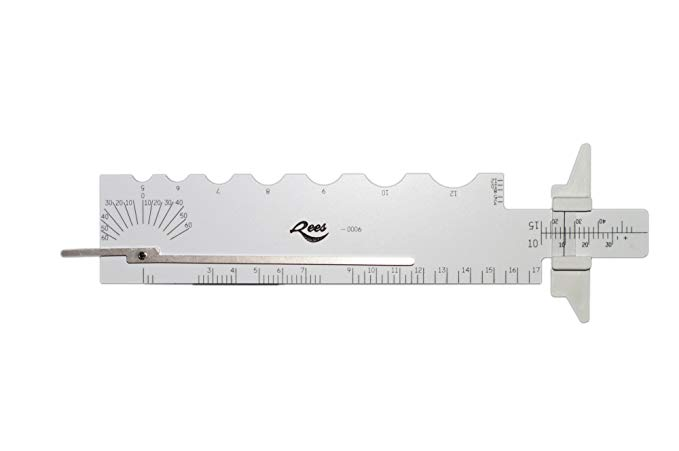
\includegraphics[width=0.8\textwidth]{obrazky-figures/fairbanks-facial-gauge.jpg}
	\caption{Fairbankův obličejový měřicí přístroj, odborný nástroj pro měření lidského obličeje \cite{Fairbank}.}
\end{figure}

\noindent Mezi další odborné měřící přístroje používané v lékařství patří kraniometr nebo kefalometr. Zmíněné pomůcky fungují na bázi kruhovitých otevíracích kleští pro měření hlavy, v různých stádiích života jedince.

\bigskip

\noindent Zaznamenávání údajů o lidském těle nám pomáhá řešit problémy (kriminalistika, antropologie, lékařství), rozvíjet poznatky o člověku a vynalézat nové použití pro fakt jedinečnosti lidské tělesné schránky (odemykání chytrého telefonu pomocí rozpoznání obličeje), je tedy důležité se v této oblasti i nadále rozvíjet a zkoumat ji.

\section{Antropometrické body a proporce}
\label{facial-landmarks}

\noindent Využití antropometrických měření je pro chirurgy zásadní při plánování operací obličeje, ať už se jedná o rekonstrukční operace po úrazech a onkologických resekcích, nebo o estetické zákroky. Nicméně použití jednoho standardu antropometrických rysů pro všechny etnické skupiny není vhodné, neboť může vést k esteticky neuspokojivým výsledkům. Proto je důležité, aby pro každou etnickou skupinu byly k dispozici specifické obličejové normy. Toho se snažil docílit profesor Leslie Gabriel Farkas, který je považován za průkopníka moderní antropometrie obličeje. On a jeho spolupracovníci zkoumali v multicentrické studii kraniofaciální charakteristiky na 25 etnických skupinách a vyvinuli měření, které obsahovalo 14 parametrů pro každou z těchto etnik \cite{Zacharopoulos2016}.

Antropometrické body (\textit{landmarks}) jsou konkrétní místa na zkoumaném subjektu, určených podle viditelných nebo hmatných znaků (kůže nebo kostí) \cite{DeCarlo1998}.

S cílem rozšířit znalosti etnické antropometrie v řecké populaci byla v roce 2015 provedena série antropometrických analýz za účelem získání významných bodů obličeje. Studie zahrnovala 152 dobrovolníků, z nichž 78 byli muži a 74 ženy ve věkovém rozmezí 18 až 30 let. Celkem bylo provedeno 31 antropometrických měření, z toho 25 jednotlivých a 3 párová. Před samotným měřením byly na obličeji každého jednotlivce vyznačeny povrchové antropometrické body z tabulky \ref{tab:landmarks}. Každé měření bylo provedeno dvakrát stejným vyšetřovatelem a následně byla použita vypočtená průměrná hodnota \cite{Zacharopoulos2016}.

\begin{figure}[H]
	\centering
	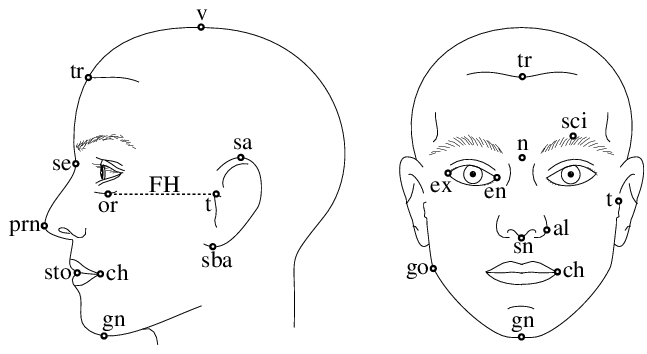
\includegraphics[width=0.95\textwidth]{obrazky-figures/Anthropometric-landmarks-on-the-face.png}
	\caption{Antropometrické body na obličeji \cite{DeCarlo1998}.}
        \label{fig:anthropometric-landmarks}
\end{figure}

\begin{table}[H]
    \centering
    \renewcommand{\arraystretch}{1.5}
    \begin{tabular}{|c|c|}
        \hline
        \textit{Glabella} (g) &  Nejvýraznější středový bod mezi obočím \\
        \textit{Opisthocranion} (op) & \makecell{Nejvzdálenější bod od bodu glabella\\
                                                    na zadní části hlavy} \\
        \textit{Trichion} (tr) & Bod na linii vlasů ve střední části čela \\
        \textit{Nasion} (n) & Bod ve střední linii kořene nosu \\
        \textit{Subnasale} (sn) & \makecell{Střední bod, kde se setkává dolní okraj \\
                                            nosní přepážky a povrch horního rtu} \\
        \textit{Gnathion} (gn) & \makecell{Nejnižší bod ve střední linii \\
                                            na dolním okraji dolní čelisti} \\
        \textit{Zygion} (zy) & Nejbočnější bod každého jařmového oblouku \\
        \textit{Gonion} (go) & Vrchol úhlu dolní čelisti \\
        \textit{Stomion} (sto) & \makecell{Pomyslný bod na křížení vertikální střední čáry obličeje \\
                                            a horizontální štěrbiny mezi jemně zavřenými rty, \\
                                            se zavřenými zuby v přirozené poloze} \\
        \textit{Endocanthion} (en) & Bod na vnitřním okraji oční štěrbiny \\
        \textit{Exocanthion} (ex) & Bod na vnějším okraji oční štěrbiny \\
        \textit{Alare} (al) & Nejbočnější bod na každém okraji nosního křídla \\
        \textit{Cheilion} (ch) & Bod umístěný na každém spojení rtů \\
        \textit{Labiale superius} (ls) & Střední bod horní linie vermilionu \\
        \textit{Labiale inferius} (li) & Střední bod spodní linie vermilionu \\
        \textit{Superaurale} (sa) & Nejvyšší bod na volném okraji ušního boltce \\
        \textit{Subaurale} (sba) & Nejnižší bod na volném okraji ušního lalůčku \\
        \textit{Tragion} (t) & Bod na horním okraji zevního zvukovodu \\
        \hline
    \end{tabular}
    \caption{Analyzované antropometrické body \cite{Zacharopoulos2016}.}
    \label{tab:landmarks}
\end{table}

Provedená měření \cite{Zacharopoulos2016} lze s pomocí tabulky \ref{tab:landmarks} a obrázku \ref{fig:anthropometric-landmarks} popsat takto:

\begin{itemize}
    \item Měření hlavy
        \begin{itemize}
            \item horizontální obvod hlavy (g-op-g),
            \item výška čela (tr-g),
            \item rozšířená výška čela (tr-n).
        \end{itemize}
    \item Měření obličeje
    \begin{itemize}
        \item oblouk horní čelisti (t-sn-t),
        \item čelistní oblouk (t-gn-t),
        \item šířka obličeje (zy-zy),
        \item šířka dolní čelisti (go-go),
        \item spodní výška obličeje (sn-gn),
        \item fyziognomická výška obličeje (tr-gn),
        \item morfologická výška obličeje (n-gn),
        \item fyziognomická výška horní části obličeje (n-sto),
        \item výška spodní třetiny obličeje (sto-gn),
        \item speciální výška obličeje (en-gn),
        \item speciální výška horního obličeje (g-sn).
    \end{itemize}
    \item Měření orbitů
    \begin{itemize}
        \item binokulární průměr (ex-ex),
        \item interkantální vzdálenost (en-en),
        \item délka oční štěrbiny (ex-en).
    \end{itemize}
    \item Měření nosu
    \begin{itemize}
        \item šířka nosu (al-al),
        \item výška nosu (n-sn),
        \item sklon nosního můstku (sklon nosu, ni).
    \end{itemize}
    \item Měření labio-orální oblasti
    \begin{itemize}
        \item šířka úst (ch-ch),
        \item mediální výška vermilionu horního rtu (ls-sto),
        \item mediální výška vermilionu dolního rtu (sto-li),
        \item mediální výška kůže horního rtu (sn-ls),
        \item mediální vertikální délka horního rtu (sn-sto).
    \end{itemize}
    \item Měření uší
    \begin{itemize}
        \item délka ucha (sa-sba),
        \item sklon mediální podélné osy ušního boltce (sklon ucha, ei).
    \end{itemize}
\end{itemize}

Po zpracování výsledků byla provedena jejich vzájemná komparace. Při porovnání mužských a ženských výsledků byly zjištěny některé významné rozdíly. Zejména výška čela (tr-g) byla zaznamenána jako extrémně menší u žen. Další rozdíly byly pozorovány v délce nosu a uší, šířce úst, velikosti a vzdálenosti očí. V těchto ohledech byly zaznamenány větší rozměry u mužů, avšak rozdíly nebyly tak výrazné jako v případě výšky čela. Horní rty byly mírně větší u řeckých žen, zatímco dolní rty byly větší u řeckých mužů \cite{Zacharopoulos2016}.

\bigskip

\noindent Další analýzou pro měření obličeje je celkový index obličeje \cite{Jeremic2013} (\textit{total facial index}, TFI). Jedná se o poměr morfologické výšky obličeje (získaný měřením vzdálenosti n-gn) a maximální šířky obličeje (vzdálenost mezi dvěma  jařmovými oblouky zy-zy). Naměřená hodnota TFI slouží k určení typu obličeje podle stupnice Martin-Saller a lze jej vypočítat podle vzorce:

\begin{equation}
    TFI = \frac{n-gn \times 100}{zy-zy}
    \label{eq:facial-index}
\end{equation}

\noindent Jednotlivé výsledky měření TFI jsou použity k určení výskytu určitých typů obličeje, rozdělené podle rozmezí hodnot umístěných v tabulce \ref{tab:tfi-categories}. Rozmezí jsou určené na základě škály Martin-Saller \cite{Jeremic2013}.

\begin{table}[H]
    \centering
    \renewcommand{\arraystretch}{1.25}
    \begin{tabular}{|c|c|}
        \hline
        Název &  Rozmezí \\
        \hline
        hypereuryprosopic & TFI $\leq$ 78,9 \\
        euryprosopic & 79,0 < TFI < 83,9 \\
        mesoprosopic & 84,0 < TFI < 87,9 \\
        leptoprosopic & 88,0 < TFI < 92,9 \\
        hyperleptoprosopic & TFI $\geq$ 93,0 \\
        \hline
    \end{tabular}
    \caption{Jednotlivé typy obličeje na základě hodnoty TFI \cite{Jeremic2013}.}
    \label{tab:tfi-categories}
\end{table}

\noindent Mimo zmíněný celkový index obličeje, existují i jiné typy poměrů obličeje, které zohledňují další proporce lidské tváře. Příkladem je poměr pro horní část obličeje.

\bigskip

\noindent Významné antropometrické body na lidském obličeji jsou klíčové pro přesné měření a analýzu obličeje, což je důležité pro mnoho aplikací. Tyto body mohou sloužit jako referenční body pro určení geometrických vlastností obličeje a umožnit tak vytvoření datových sad pro trénování algoritmů strojového učení, stejně jako poskytují cenný zdroj pro chirurgy specializující se na operace obličeje. Takové datové sady jsou základem pro vývoj a zdokonalování technologií spojených s obličejem, které naleznou využití například v biometrii, zábavním průmyslu, medicíně nebo bezpečnostních aplikacích.

\chapter{Neuronové sítě pro generování syntetických snímků obličeje}
\label{neural}

Neuronové sítě (angl. \textit{neural networks}), známé také jako \bf umělé neuronové sítě \rm \cite{IBMANN} (angl. \textit{artificial neural networks}), jsou podmnožinou strojového učení (angl. \textit{machine learning}) -- procesu trénování počítačových programů a jsou základem algoritmů hlubokého učení (angl. \textit{deep learning algorithms}). Jejich název a struktura jsou inspirovány lidským mozkem, protože napodobují způsob, jak si biologické neurony mezi sebou předávají signály. Umělé neuronové sítě se rozvíjejí v různých směrech, nabízející tak specifická využití v konkrétních oblastech. Mezi ně patří i generativní neuronové sítě, které jsou určeny pro tvorbu nového obsahu nebo modifikaci již existujícího. 

\bigskip

\noindent Neuronové sítě jsou prostředkem \bf strojového učení\rm, ve kterém se počítač učí provádět určitý úkol na základě analýzy trénovacích případů. Příklady jsou obvykle ručně označeny -- například vložím obrázek do rozpoznávacího systému a označím, co se na obrázku nachází, to stejné mohu udělat s celou sadou obrázků. 

Na základě uživatelem dopředu vytvořených označení, je umělá inteligence schopná se učit, které výsledky provedla správně a vytvoří si v případě detekce objektu -- vizuální vzory, které konzistentně korelují s určitými označeními a bude se jimi řídit dále (například u obrázků auta detekuje, že častým jevem jsou kola, proto se na tuhle oblast začne soustředit a dojde k přesnějším výsledkům). Čím více takových dat, tím přesnější se umělá inteligence může stát \cite{MITNN}.

Umělá inteligence zaměřená pouze na jeden úkol se nazývá \textit{artificial narrow intelligence}, opakem pak je \textit{artificial general intelligence}, které nemá konkrétní zaměření -- na jejím vývoji se momentálně pracuje.

\section{Úvod do neuronových sítí}
\label{neural-intro}

Neuronové sítě se skládají z uzlových vrstev, které obsahují vstupní vrstvu (angl. \textit{input layer}), jednu nebo více skrytých vrstev (angl. \textit{hidden layers}) a výstupní vrstvu (angl. \textit{output layer}). Každý uzel se připojuje k jinému uzlu a má přiřazené váhy (angl. \textit{weight}) a práh (angl. \textit{threshold}). Pokud je hodnota některého z jednotlivých výstupu vyšší než stanovená prahová hodnota, aktivuje se uzel a předávají se data do následující vrstvy. V případě, že toto neplatí, nedochází k dalšímu předávání dat \cite{IBMANN}. 

\bigskip

\noindent \bf Perceptron \rm \cite{Perceptron} je jednovrstvá neuronová síť. Vícevrstvý perceptron se označuje jako neuronové sítě (\textit{neural networks}), ty ve své podstatě fungují stejně jako perceptron. Sestává z 4 klíčových částí:

\begin{enumerate}
    \item vstupní hodnoty ($x_{n}$),
    \item váhy ($w_{0}...w_{n}$),
    \item součet násobení jednotlivých vstupů se svými váhami ($\sum$),
    \item aktivační funkce.
\end{enumerate}

\begin{figure}[H]
	\centering
	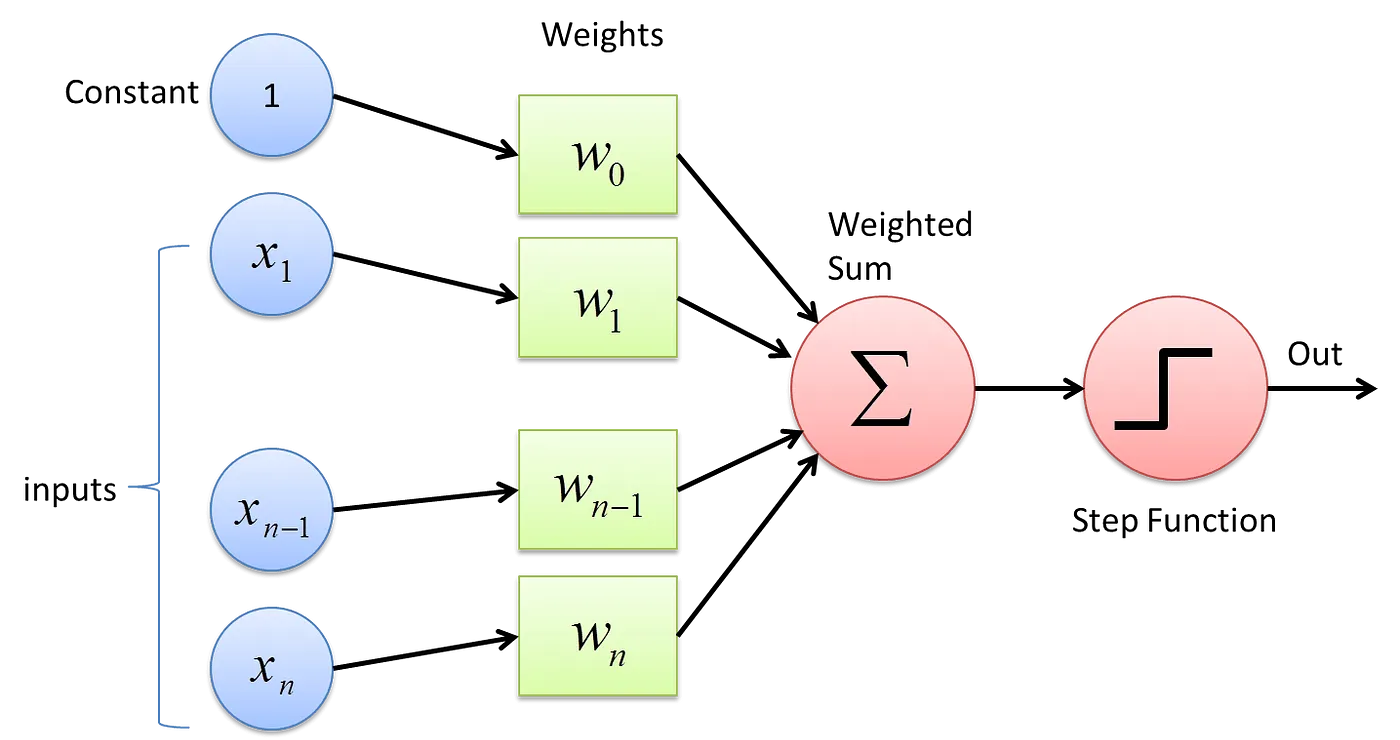
\includegraphics[width=0.8\textwidth]{obrazky-figures/perceptron.png}
	\caption{Model procesu perceptronu \cite{Perceptron}.}
\end{figure}

\noindent Všechny vstupy ($x_{n}$) jsou vynásobeny s jejich váhami ($w_{n}$), výsledek operace $x_{n}w_{n}$ může být nazýván například $k$. Nad těmito výsledky $k$  je následně provedena suma, ke které je možné přičíst i nějakou odchylku (\textit{bias} $b$): 

\[ sum = \sum_{i=0}^n k_i + b \]

Získaná hodnota $sum$ je aplikována na aktivační funkci, která obsahuje určitý práh, určující výstup v souladu s typem zvolené aktivační funkce (např. lineární, skoková, sigmoidní, ReLU, \dots). 

\bigskip

\noindent Ztrátová funkce \cite{LossFunctions} (\textit{loss function}) je nástrojem pro hodnocení účinnosti algoritmů strojového učení ve vztahu k datové sadě. Konkrétně měří, jak přesně algoritmus dosahuje zamýšlených výsledků a vyjadřuje, jak úspěšně představuje daný výsledek. Čím nižší je hodnota ztrátové funkce, tím je model přesnější, protože naznačuje menší rozdíl mezi očekávanými a předpovězenými výsledky. V průběhu trénování se váhy a parametry modelu mění tak, aby byla minimalizována hodnota ztrátové funkce.

Existuje mnoho typů ztrátových funkcí, z nichž každá je vhodná pro určité úlohy strojového učení. Pro klasifikační úlohy často používaná křížová entropie (\textit{cross-entropy}), která měří rozdíl mezi pravdivými a předpovězenými pravděpodobnostmi tříd. V regresních úlohách, kde se předpovídají kontinuální hodnoty, se často uplatňuje střední kvadratická chyba (\textit{Mean Squared Error}) \cite{LossFunctions}.

\bigskip

\noindent Třívrstvá neuronová síť představuje pokročilý model umělé inteligence, který vychází z~konceptu perceptronu, avšak zahrnuje více vrstev pro komplexnější zpracování informací. Tato síť se skládá ze tří hlavních vrstev: vstupní vrstvy, skryté vrstvy a výstupní vrstvy.

Zpětné šíření (\textit{backpropagation}) je klíčovým mechanismem učení neuronových sítí. Po prezentaci vstupních dat a generování odpovědi výstupní vrstvou dochází k porovnání této odpovědi s očekávanými výstupy. Chybový signál se pak šíří zpětně skrz síť a upravuje váhy mezi neurony, aby se minimalizovala chyba predikce. Tímto způsobem síť postupně optimalizuje své váhy a dosahuje lepší schopnosti generování nových dat. Opakem \textit{backpropagation} je \textit{feedforward} šíření, které postupuje jedním směr od vstupu do výstupu \cite{IBMANN}.

\bigskip

\noindent Dalším zásadním pojmem je hluboké učení (\textit{deep learning}). Rozdíl mezi \textit{deep learning} a neuronovými sítěmi nemusí být ale vždy jasný. Oba termíny spolu souvisí a mohou se prolínat -- \uv{hloubka} v hlubokém učení značí hloubku vrstev v neuronové síti, tedy to jak moc je neuronová síť rozsáhlá. 

Neuronová síť, která je složená \bf z více než tří vrstev \rm (včetně vstupní a výstupní vrstvy), \bf může být brána jako algoritmus hlubokého učení \rm (angl. \textit{deep learning algorithm}), v opačném případě (3 nebo méně vrstev, včetně) se jedná jen o základní neuronovou síť \cite{IBMANN}.

\begin{figure}[H]
	\centering
	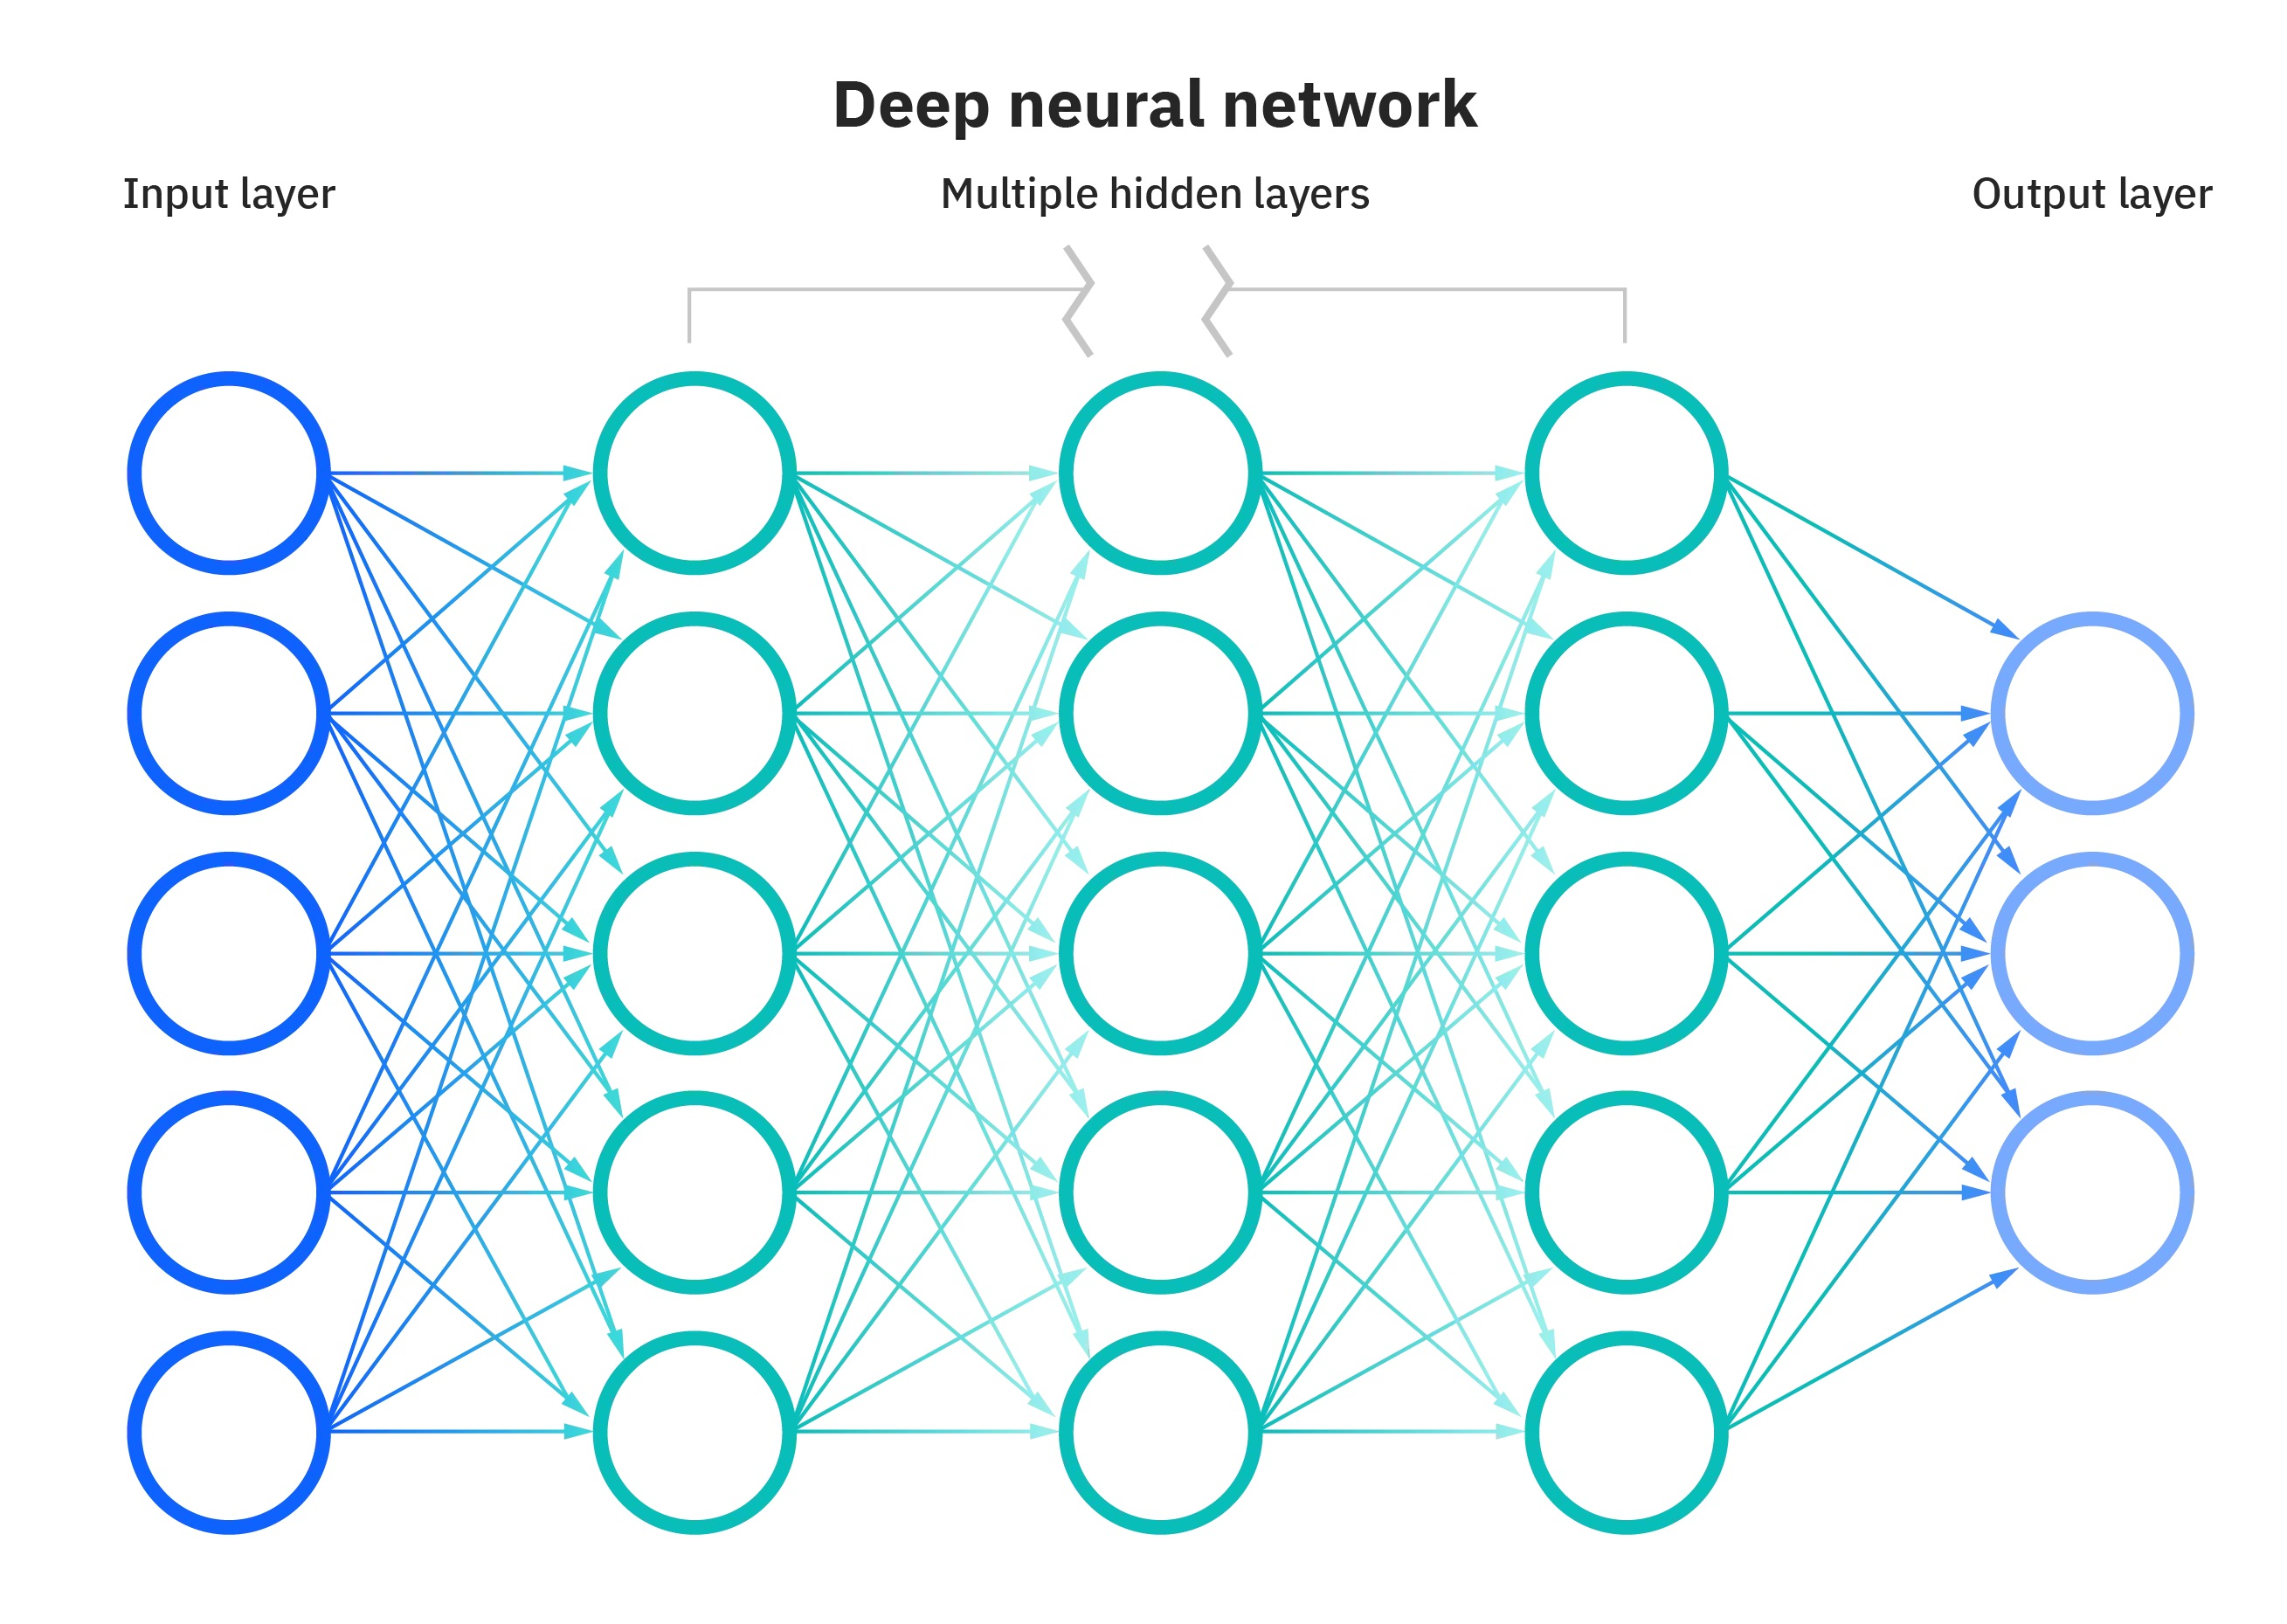
\includegraphics[width=0.8\textwidth]{obrazky-figures/DNN.jpeg}
	\caption{\textit{Deep learning} neuronová síť s několika skrytými vrstvami \cite{MediumDNN}.}
        \label{fig:DNN}
\end{figure}

\subsection*{Konvoluční neuronové sítě}

Pojem, který se bude hojně vyskytovat v kapitole \ref{section-gan} je konvoluce \cite{weisstein2003convolution}, respektive \textbf{konvoluční vrstva} \cite{ElementCNN}. V případě, že neuronová síť obsahuje tuto konvoluční vrstvu, je referována jako konvoluční neuronová síť. Tato vrstva slouží k počítačovému zpracování obrazu, a jejím hlavním přínosem je schopnost detekce prvků na snímku, jako jsou světlé nebo tmavé (nebo specificky zbarvené) body, okraje v různých orientacích, vzory atd. Tyto identifikované prvky následně odhalují významné objekty na obrázku, například lidské oko, nos, ústa a další. 

Hlavním cílem konvoluční vrstvy je tedy schopnost rozeznat objekty na obrázcích, nezávisle na jejich umístění, natočení a osvětlení. To zároveň snižuje velikost potřebné trénovací sady. Konvoluční vrstvy se často nacházejí až ve spodních vrstvách neuronových sítí \cite{ElementCNN}.

\bigskip

\noindent Podle vzoru lidského mozku se neuronová síť skládá z tisíců nebo dokonce milionů jednoduchých výpočetních uzlů -- neuronů, které jsou hustě propojeny. Většina dnešních neuronových sítí je uspořádána do vrstev uzlů a pracuje podle principu \textit{feed-forward}. Na obrázku \ref{fig:DNN} lze vidět, že jednotlivý uzel může být propojen s několika uzly ve vrstvě nižší (podle obrázku se jedná o uzly nalevo od daného uzlu), od kterých přijímá data, a s několika uzly ve vrstvě vyšší (uzly napravo od daného uzlu), kam data posílá \cite{MITNN}.

\section{Generativní neuronové sítě}

Generativní neuronové sítě \cite{MediumAI} patří mezi klíčové nástroje v oblasti strojového učení. Jedná se o neřízené nebo částečně řízené strojové učení pro vytváření nového obsahu -- především v~oblasti digitálních obrázků, videí, zvuku, textu a zdrojového kódu. Tyto sítě jsou navrženy tak, aby mohly vytvářet nový obsah na základě vzorů a dat, která byla před nimi prezentována. Jsou to modely, které se snaží pochopit a replikovat vzory v datech, aby mohly generovat nový obsah, který je podobný těmto vzorům, ale zároveň je i originální.

\bigskip

\noindent Jedním ze zástupců generativní umělé inteligence dosáhl v posledních letech vrcholu popularity, mluvíme o \textit{Generative Pre-trained Transformer}, více známý pod zkratkou \bf GPT\rm, u kterého se jedná o auto-regresivní jazykový model založený na architektuře transformátoru. Je dopředu trénovaný, ale není již pod dohledem (není supervizován). Tento model je známý především díky produktu GPT-3.5 (a GPT-4) od společnosti OpenAI, spuštěný v~roce 2022~\cite{MediumAI}.

\bigskip

\noindent Mimo GPT zde existuje další velký sektor umělých neuronových sítí -- jedná se \textit{Generative Adversarial Network} (Generativní adverzní sítě) ve zkratce \bf GAN \rm \cite{goodfellow2014generative}. Tyto sítě využívají dvě neuronové sítě, které umožňují si navzájem předávat informace pro učení a tím zdokonalovávat model. Princip konkurenčního učení mezi těmito sítěmi vedl k významným pokrokům v oblasti generativního umění, což zahrnuje generování obrázků, videa a audia s~vysokou úrovní autentičnosti a estetiky. GAN sítě tak představují další mocný nástroj pro tvorbu obsahu, který umožňuje vytvářet realistické a nápadité digitální výstupy \cite{goodfellow2014generative}\cite{MediumAI}.

Jejich použití je možné vidět v oblasti marketingu a reklamy, kde generativní modely mohou pomoci vytvářet personalizovaný obsah pro zákazníky, ve video produkci pro tvorbu realisticky vypadajících videí přizpůsobených potřebám tvůrce, v hudbě pro generování nových hudebních kompozic a zvukových efektů nebo v umění a kultuře pro tvorbu originálních uměleckých děl.


\subsection*{Generativní adverzní sítě}
\label{section-gan}

\textit{Generative Adversarial Network} \cite{goodfellow2014generative} je rámec strojového učení pro tvorbu vizuální obsahu. Využívá dvě neuronové sítě, které spolu \uv{soutěží} a vzájemně se zlepšují prostřednictvím svého soupeřivého vztahu. První neuronovou sítí je \bf generátor \rm($G$), který zachycuje distribuci dat, a k němu \bf diskriminační model \rm($D$), který odhaduje pravděpodobnost, zda vzorek pochází z trénovacích dat, a ne z modelu $G$.

\bigskip

\noindent Oba modely se navzájem zlepšují. Model $G$ poskytuje modelu $D$ data, která $D$ využívá k přesnějšímu určení věrohodných informací, respektive model $D$ se učí rozeznat, jestli vzorek pochází z distribučního modelu $G$, nebo z předem určené datové sady (vizuálně jde proces vidět na obrázku \ref{fig:GAN}). Hlavním cílem modelu $G$ je však maximalizovat pravděpodobnost, že $D$ udělá chybu. Tímto způsobem se $G$ snaží stát více věrohodným modelem. Model $D$ poskytuje zpětnou vazbu ohledně věrohodnosti generovaných dat a tím posiluje věrohodnost modelu $G$, což vede k vytváření kvalitnějších a spolehlivějších dat.

Lze také použít analogii, ve které je generativní model $G$ skupina padělatelů, kteří se snaží vytvořit falešné peníze, aniž by se na to přišlo. Diskriminační model $D$ reprezentuje policejní trestní orgán, která se snaží odhalit tyto padělané peníze. Obě strany mají motivaci zlepšovat se, s cílem předčit své vzájemné protějšky \cite{goodfellow2014generative}\cite{GANgoogle}.

\begin{figure}[H]
	\centering
	\includesvg[width=1\textwidth]{obrazky-figures/gan_diagram.svg}
	\caption{GAN diagram obsahující model generátoru, generující výsledky z dat získaných na vstupu a diskriminační model, určující věrohodnost získaných vstupů od generátoru a datové sady. Postavené na bázi hry pro 2 -- minimax \cite{GANgoogle}.}
        \label{fig:GAN}
\end{figure}

\noindent Celý proces odpovídá algoritmu minimax mezi 2 hráči. V případě, že jsou $G$ a $D$ definovány pomocí vícevrstvých perceptronů, lze celý systém trénovat pomocí \textit{backpropagation} algoritmu (zpětné šíření), jejímž prostřednictvím poskytuje diskriminační klasifikátor $D$ signály, které generátor $G$ používá k aktualizaci svých vah \cite{goodfellow2014generative}\cite{GANgoogle}. 

Zmíněná minimax hra pro dva hráče ($D$ a $G$) s hodnotovou funkcí $V(G, D)$, lze vyjádřit vzorcem

\begin{equation}
    \min_G \max_D V(D, G) = \mathbb{E}_{\mathbf{x} \sim p_{\text{data}}(\mathbf{x})} [\log D(\mathbf{x})] + \mathbb{E}_{\mathbf{z} \sim p_\mathbf{z}(\mathbf{z})} [\log(1 - D(G(\mathbf{z})))]
    \label{eq:GANminimax}
\end{equation}

kde $G$ je generativní model a $D$ je model diskriminační, v obou případech je model vícevrstvý perceptron, v opačné situaci není možné rámec použít. $x$ představuje vzorky reálných dat a $z$ představuje vstupní proměnné šumu, které jsou vzorkovány z rozdělení s prioritou. $p_{\text{data}}(\mathbf{x})$ označuje skutečné rozdělení dat, $p_\mathbf{z}(\mathbf{z})$ označuje rozdělení šumu. Výstupem rovnice \eqref{eq:GANminimax} je jeden skalární výraz.

\textit{Loss function} se vyskytuje jak u generativního modelu $G$, tak u modelu diskriminačního $D$. U generátoru označuje, do jaké míry se podařilo oklamat diskriminační model pomocí vygenerovaného výsledku. Na straně diskriminačního modelu jde o to, jak efektivně dokázal odhalit rozdíl mezi reálným vzorkem a tím, který byl vytvořen generátorem. Další obecné informace k pojmu \textit{loss function} se nachází v sekci \ref{neural-intro}.

\bigskip

\noindent GAN je rámec generativních neuronových sítí, umožňující generování vizuálního a audio obsahu. Je složen ze dvou neuronových sítí, které proti sobě soupeří ve hře minimax a navzájem se zdokonalují. Výhody zahrnují to, že nikdy není potřeba Markovův řetězec, během učení není potřeba žádná odvozovací metoda, k získání gradientů se používá pouze zpětné řízení a do modelu lze začlenit širokou škálu funkcí. Nevýhodou je, že $D$ musí být během trénování dobře synchronizované s $G$, zejména $G$ nemůžeme být příliš trénováno, aniž by se neaktualizovalo $D$. To může způsobit, že trénink bude nestabilní a pomalý \cite{goodfellow2014generative}.

\section{Generování syntetických snímků obličeje umělou inteligencí}

V současné době se GAN používají v různých oblastech výzkumu a aplikací, jako je generování obrazu, překreslování obrazu, generování textu, zpracování lékařských snímků, segmentace obrazu, barevné zobrazení, převod obrazu na obraz a tvorba uměleckých děl. Kromě toho se GAN hojně využívají při \bf syntéze a úpravě obličejů\rm, například při určování věku a pohlaví osob. 

V posledních letech je syntéza snímků obličeje žhavým tématem v oblasti zpracování fotografií, vzhledem k častému využívání snímků na sociálních sítích. Zpracování obrazů obličeje dosáhlo díky zlepšení výkonu GAN velkého pokroku. Objevila se řada metod pro zlepšení kvality generování obrazu obličeje. Následující modely, představují současný stav generování lidského obličeje umělými neuronovými sítěmi. Často tyto modely pracují na základě zpracování atributů v obrázku a jejich úpravě \cite{reviewGANs}. 

\newpage

\subsection*{ELEGANT}

Nástroj ELEGANT poskytuje model, který umožňuje přenos více atributů obličeje, umožňující na snímku lidské tváře například odstranění ofiny, změny barvy vlasů nebo změny mužských rysů na ženské. Schéma rámce lze vidět na obrázku \ref{fig:elegant}.

\begin{figure}[H]
	\centering
	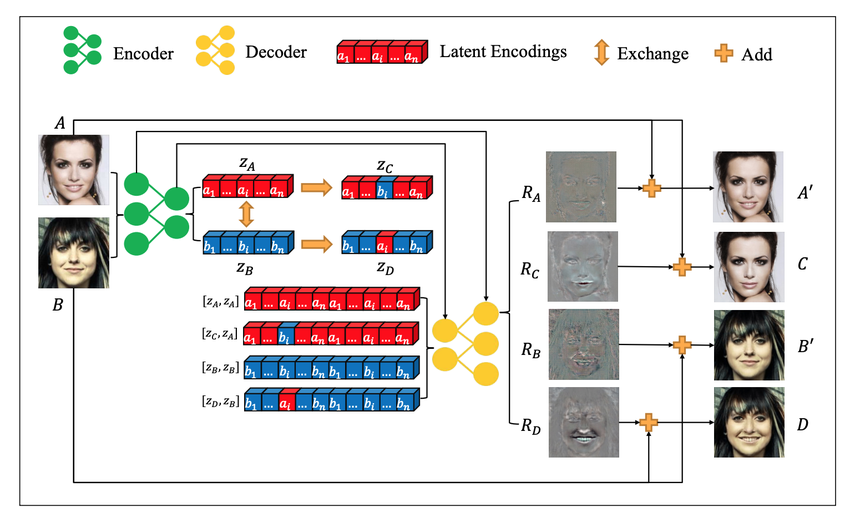
\includegraphics[width=0.9\textwidth]{obrazky-figures/schemeElegant.png}
	\caption{Struktura modelu ELEGANT pro změnu atributů a následnou syntézu snímků obličeje \cite{elegant-scheme}.}
        \label{fig:elegant}
\end{figure}

\noindent \textit{Loss function} diskriminátoru $D$

\begin{equation}
    L_{D} =L_{D_{1}} +L_{D_{2}}
    \label{eq:ELEGANTDis}
\end{equation}

kde $L_D$ značí ztrátu diskriminátoru, $L_{D_{1}}$ a $L_{D_{2}}$ značí ztráty více-škálových diskriminátorů \cite{elegant-scheme}.

\bigskip

\noindent \textit{Loss function} generátoru $G$

\begin{equation}
    L_{G} =L_{reconstruction} +L_{adv}
    \label{eq:ELEGANTGen}
\end{equation}

kde $L_{G}$ značí ztrátu generátoru, $L_{reconstruction}$ ztrátu rekonstrukce a $L_{adv}$ nepříznivou ztrátu \cite{elegant-scheme}.

\bigskip

\noindent ELEGANT představuje účinnou metodu pro přenos atributů obličeje. Jako vstupy přijímá dva obrazy s opačnými atributy a dokáže vytvořit vysoce kvalitní snímky s drobnými detaily. Dále umožňuje výměnu specifických kódových částí, což umožňuje přenést stejné atributy z jednoho obrázku na druhý. Tato metoda může manipulovat s několika atributy současně tím, že zakóduje různé atributy do nespojitých částí v latentním prostoru. To znamená, že je možné provést změny například v barvě vlasů a současně upravit tvar nosu \cite{reviewGANs}.

\newpage

\subsection*{StarGAN}

StarGAN \cite{choi2018stargan} je model vytvořený Y. Choi, umožňující vytvářet nové snímky v rámci multidoménového překladu, za pomocí jen jednoho modelu. Tato vlastnost poskytuje ještě flexibilnější možnost generování obrázků.

\begin{figure}[hbt]
	\centering
	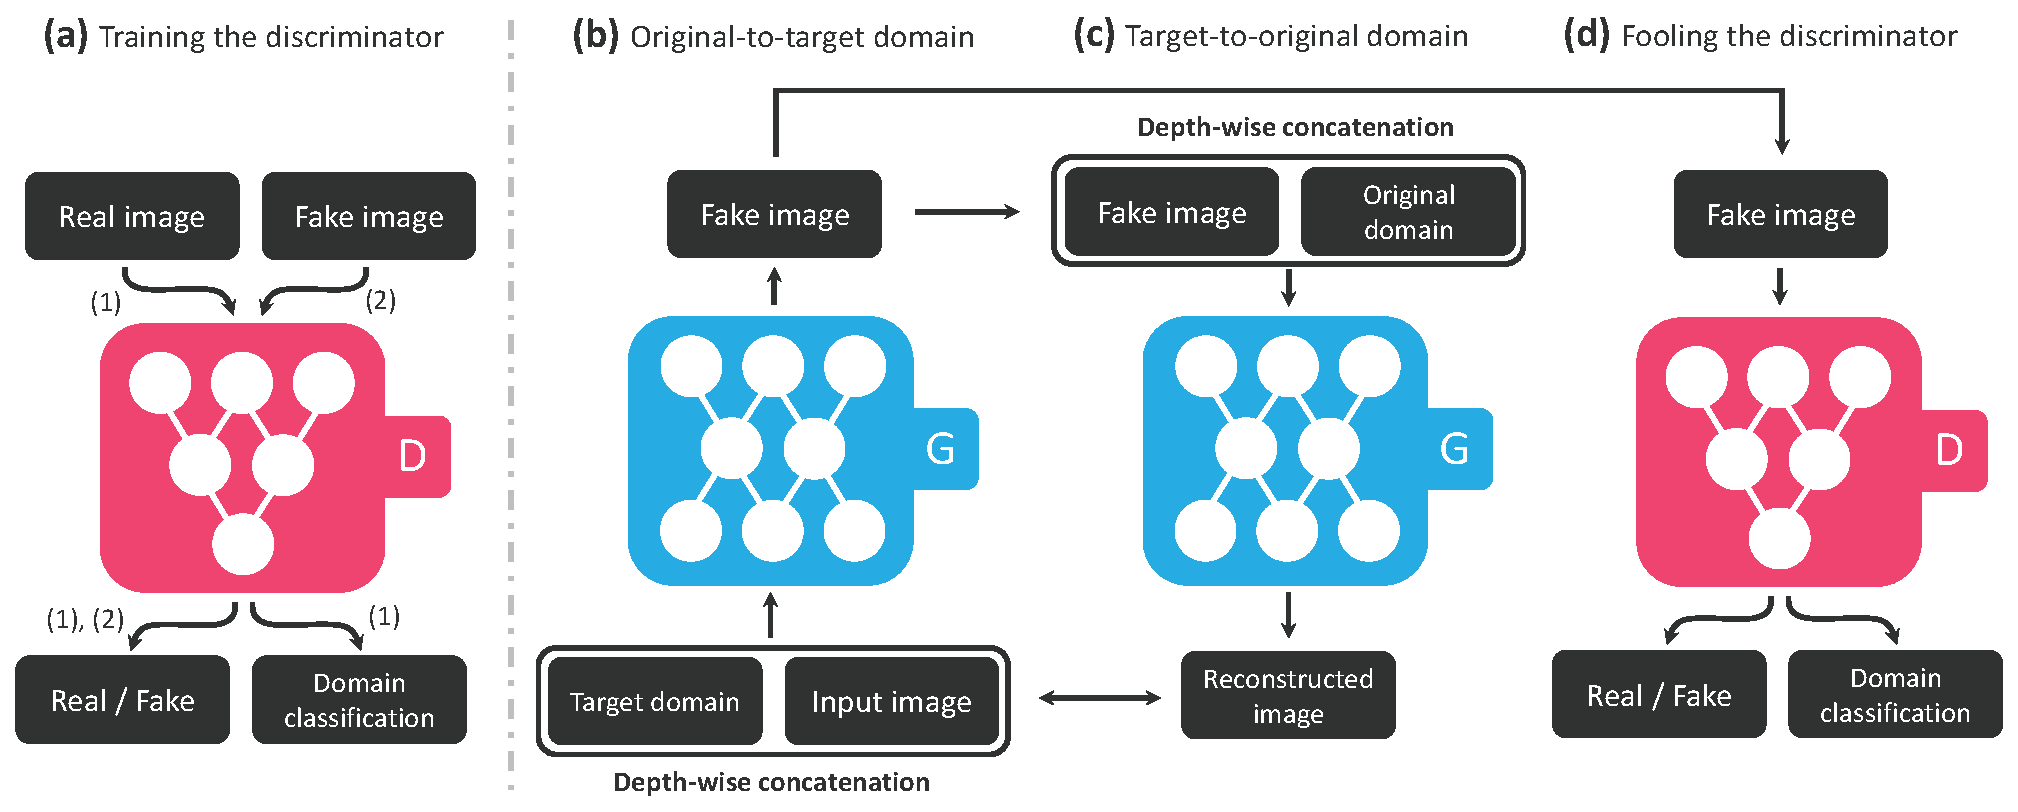
\includegraphics[width=1\textwidth]{obrazky-figures/stargan_overview.pdf}
	\caption{Přehled sítě StarGAN \cite{choi2018stargan}.}
        \label{fig:stargan}
\end{figure}

\noindent StarGAN se skládá ze dvou částí -- generátoru $G$ a diskriminátoru $D$. $D$ je trénován nad sadou obrázků, štítkovaných s informací o jejich původu. $G$ se snaží generovat obrázky, tak aby $D$ neodhalil, že se nejedná o reálné obrázky.

\noindent\textit{Loss function} modelu StarGAN

\begin{align}
    \mathcal{L}_{D} =  - \mathcal {L}_{adv} +  {\lambda}_{cls}\thinspace\mathcal{L}_{cls}^{r}, \\
    \mathcal{L}_{G} =   \mathcal {L}_{adv} +  {\lambda}_{cls}\thinspace\mathcal{L}_{cls}^{f} + 
    {\lambda}_{rec}\thinspace\mathcal{L}_{rec},
    \label{eq:StarGANObj}
\end{align}

kde $\mathcal{L}_{D}$ značí ztrátu diskriminátoru a $\mathcal{L}_{G}$ ztrátu generátoru. $\mathcal {L}_{adv}$ představuje nepříznivou ztrátu (\textit{Adversarial Loss}), $\mathcal{L}_{cls}^{r}$ ztrátu klasifikace domény (\textit{Domain Classification Loss}) a $\mathcal{L}_{rec}$ ztrátu při rekonstrukci (\textit{Reconstruction Loss}). ${\lambda}_{cls}$ a ${\lambda}_{rec}$ jsou hyperparametry, které řídí relativní důležitost klasifikačních a rekonstrukčních ztrát v doméně v porovnání s nepříznivou ztrátou \cite{choi2018stargan}.

\bigskip

\noindent Generátor se učí ignorovat nespecifikované označení a zaměřuje se na ty, která byla určena. Architektura tohoto modelu částečně vychází z konceptu modelu CycleGAN. Generátor je utvářen dvěma konvolučními vrstvami s velikostí kroku dva pro \textit{downsampling}, šesti zbytkovými bloky a dvěma transponováními konvolučními vrstvami s velikostí kroku dva pro \textit{upsampling}. Model slouží pro škálovatelný převod \textit{image-to-image} (obrazu na obraz) mezi více doménami pomocí jediného generátoru a diskriminátoru \cite{choi2018stargan}. 

\newpage

\subsection*{STGAN}

Nástroj \textit{Spatio-Temporal} GAN slouží pro editaci obličejových atributů, dosahující vysoce kvalitní stupeň výsledků úprav.

\begin{figure}[H]
	\centering
	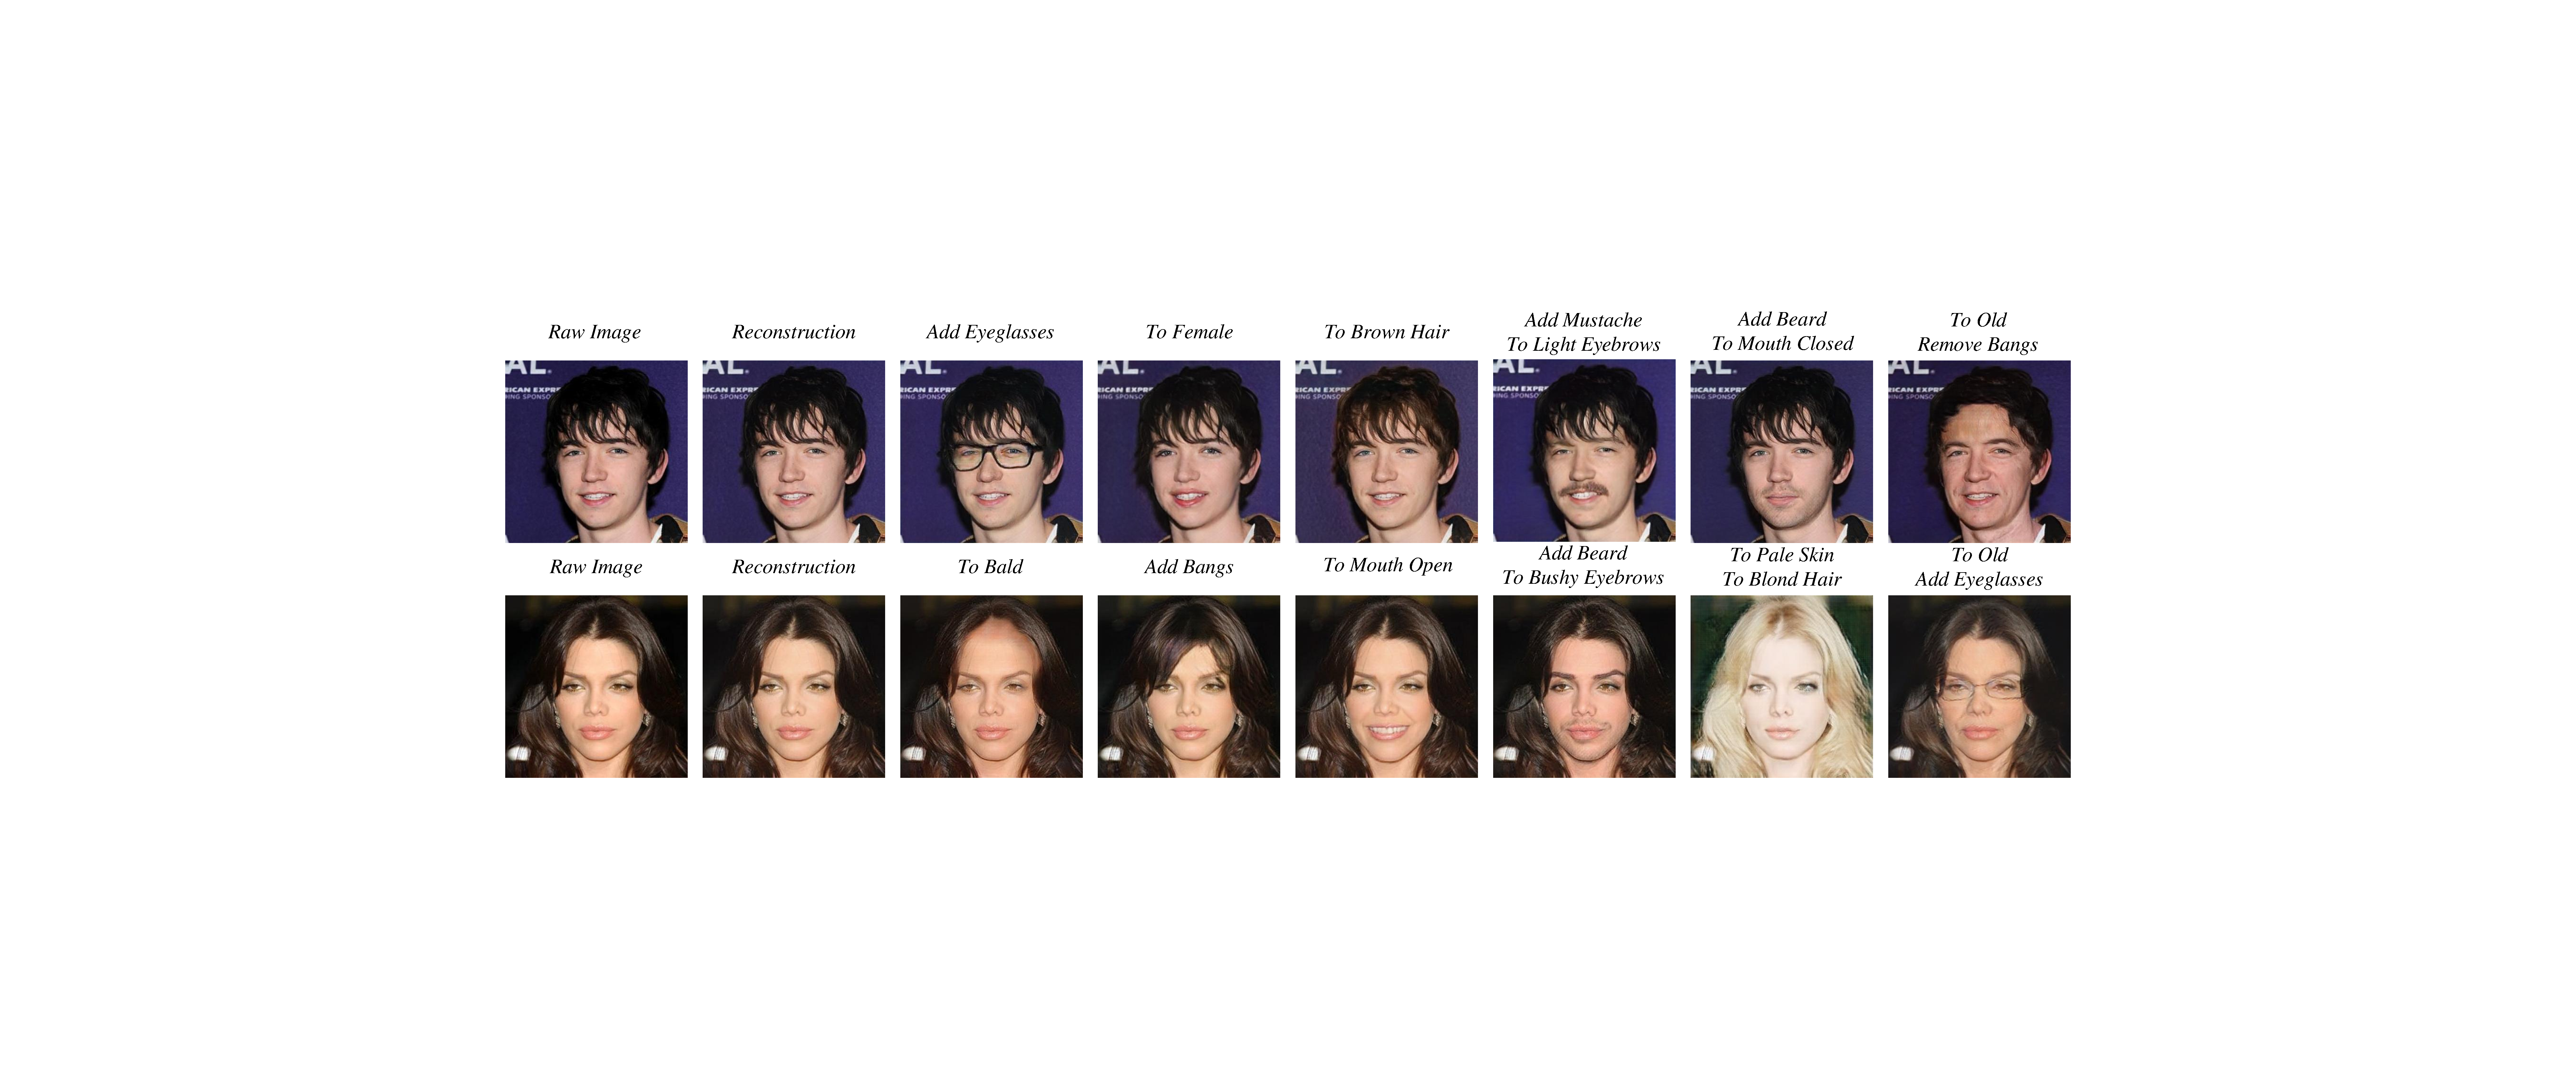
\includegraphics[width=1\textwidth]{obrazky-figures/face_HD2_.pdf}
	\caption{Výsledky STGAN pro úpravu atributů obličeje \cite{liu2019stgan}.}
        \label{fig:stgan}
\end{figure}

\noindent \textit{Loss function} modelu STGAN

\begin{align}
    \min \limits _{D} \mathcal{L}_{D} =-\mathcal{L}_{D_{adv}} +\lambda _{1} \mathcal{L}_{D_{att}} \\
    \min \limits _{G} \mathcal{L}_{G} =-\mathcal{L}_{G_{adv}} +\lambda _{2} \mathcal{L}_{G_{att}} +\lambda _{3} \mathcal{L}_{rec}
    \label{eq:STGAN}
\end{align}

kde $L_D$ značí ztrátu diskriminátoru a $\mathcal{L}_G$ ztrátu generátoru. $\mathcal{L}_{D_{adv}}$ a $\mathcal{L}_{G_{adv}}$ jsou nepříznivé ztráty, $\mathcal{L}_{D_{att}}$ a $\mathcal{L}_{G_{att}}$ jsou ztráty při manipulaci s atributy a $\mathcal{L}_{rec}$ je rekonstrukční ztráta. $\lambda _{1}$, $\lambda _{2}$, $\lambda _{3}$ jsou parametry kompromisu modelu \cite{liu2019stgan}.

\bigskip

\noindent Tato metoda řeší jemnou kontrolu označení atributu obličeje a realizuje transformaci více atributů. Model bere jako vstup vektor rozdílových atributů a v konkrétních editačních úlohách mění související atributy namísto všech cílových atributů. STGAN je vysoce přesný model pro editaci atributů založený na modelu StarGAN \cite{choi2018stargan}. Autoři navrhli selektivní přenosové jednotky (\textit{selective transfer units}) pro zlepšení editace atributů, které mohou zlepšit přesnost manipulace s atributy a zlepšit kvalitu zobrazení. STGAN může zlepšit kvalitu generovaných obrazů a realizovat flexibilní překlad atributů tím, že se primárně zaměří na úpravu atributů, které mají být změněny \cite{reviewGANs}.

\newpage

\subsection*{SGGAN}

Model \textit{Segmentation Guided Generative Adversarial Networks} od autora S. Jiang pro překlad obrazu obličeje s více doménami.

\begin{figure}[H]
	\centering
	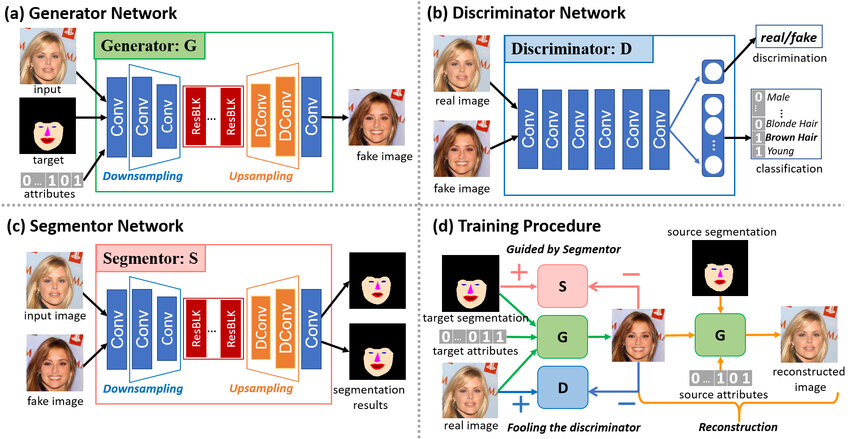
\includegraphics[width=1\textwidth]{obrazky-figures/struct-sggan.png}
	\caption{Struktura modelu SGGAN -- a) generátor G, b) diskriminátor D, c) segmentátor S, během tréninku S poskytuje G prostorové pokyny, aby se zajistilo, že generované obrazy odpovídají vstupním segmentacím, d) tréninková procedura zajišťující realistický výstup \cite{sggan}.}
        \label{fig:sggan}
\end{figure}

\noindent \textit{Loss function} modelu SGGAN

\begin{align}
    \mathcal{L}_{S}=&\mathcal{L}_{seg}^{real} \\[-1pt]
    \mathcal{L}_{D}=&-\mathcal{L}_{adv} +\lambda _{1} \mathcal{L}_{cls}^{real} \\[-1pt]
    \mathcal{L}_{G}=&\mathcal{L}_{adv} +\lambda _{1} \mathcal{L}_{cls}^{fake} +\lambda _{2} \mathcal{L}_{seg}^{fake} +\lambda _{3} \mathcal{L}_{rec}
    \label{eq:SGGANObj}
\end{align}

kde $\mathcal{L}_{S}$ je ztráta segmentoru sítě, $\mathcal{L}_D$ je ztráta diskriminátoru a  $\mathcal{L}_{G}$ je ztráta generátoru. $\mathcal{L}_{seg}^{real}$ a $\mathcal{L}_{seg}^{fake}$ jsou segmentační ztráty, $\mathcal{L}_{adv}$ je nepříznivá ztráta.  $\mathcal{L}_{cls}^{real}$ a $\mathcal{L}_{cls}^{fake}$ jsou klasifikační ztráty a $\mathcal{L}_{rec}$ je rekonstrukční ztráta. $\lambda _{1}$, $\lambda _{2}$, $\lambda _{3}$ jsou hyperparametry, které řídí váhy klasifikační ztráty, segmentační ztráty a rekonstrukční ztráty \cite{sggan}.

\bigskip

\noindent Metoda je založena na hlubokém generativním modelu, který věnuje pozornost informacím vyšší úrovně a specifickým informacím o instancích a dokáže generovat realistické obrazy vysoké kvality. Má prostorovou kontrolu v procesu překladu obrazu tím, že využívá sémantickou segmentaci ke zlepšení výkonu generování obrazu a poskytuje prostorové mapování. Umožňuje zlepšit kvalitu generování obrazu díky schopnosti prostorové modifikace \cite{reviewGANs}.

\newpage

\subsection*{MaskGAN}

Manipulace s obrazy obličeje dosáhla v posledních letech velkého pokroku. Předchozí metody však buď pracují s předem definovanou sadou atributů obličeje, nebo ponechávají uživatelům jen malou volnost při interaktivní manipulaci s obrázky. K překonání těchto nedostatků navrhujeme nový rámec označovaný jako MaskGAN, který umožňuje rozmanitou a interaktivní manipulaci s obličeji \cite{CelebAMask-HQ}.

\begin{figure}[hbt]
	\centering
	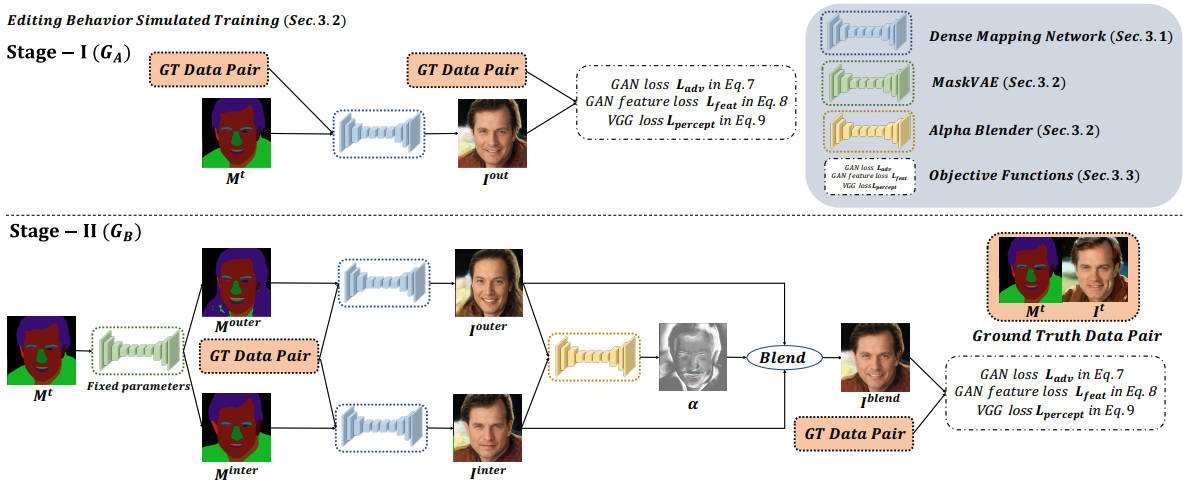
\includegraphics[width=1\textwidth]{obrazky-figures/struct-maskgan.png}
	\caption{Celkový tréninkový proces u MaskGAN. Úprava chování simulovaného tréninku lze rozdělit do dvou fází. Po načtení předtrénovaného modelu husté mapovací sítě a MaskVAE tyto dvě fáze iterativně aktualizujeme, dokud model nekonverguje \cite{CelebAMask-HQ}.}
        \label{fig:maskgan}
\end{figure}

\noindent \textit{Loss function} modelu MaskGAN:

\begin{align}
    \mathcal{L}_{G_{A},G_{B}} =& \mathcal{L}_{adv} (G,D_{1,2})+\lambda _{feat} \mathcal{L}_{feat} (G,D_{1,2}) \\&~ \qquad \qquad \qquad \qquad
    {+\,\lambda _{percept} \mathcal{L}_{percept} (G)\,\,}
    \label{eq:MaskGANObj}
\end{align}

kde $G$ je generátor, $D$ je diskriminátor a $\mathcal{L}_G$ je ztráta generátoru. $\mathcal{L}_{adv}$ je podmíněná nepříznivá ztráta, která zvyšuje realističnost generovaných obrazů a opravuje strukturu generování. $\mathcal{L}_{feat}$ je ztráta při porovnávání prvků a $\mathcal{L}_{percept}$ je percepční ztráta, která zlepšuje generování obsahu od nízkofrekvenčních k vysokofrekvenčním detailům ve vnímání směrem k hlubokým rysům. $\lambda _{feat}$ a $\lambda _{percept}$ jsou parametry pro úpravu ztráty \cite{CelebAMask-HQ}.

\bigskip

\noindent Tato metoda překonává omezení spojená s práci s předem definovaným souborem obličejových atributů. Využití sémantických masek jako reprezentace umožňuje uživatelům manipulaci s obrazovými daty obličejů s větší svobodou a interaktivitou. Rámec MaskGAN umožňuje flexibilní manipulaci s obličejovými snímky a zároveň zachovává věrnost původnímu obrazu \cite{reviewGANs}.

V rámci vývoje MaskGANu byl vytvořen rozsáhlý soubor dat o tvářích s vysokým rozlišením a jemnými anotacemi masek, nazvaný CelebAMask-HQ \cite{CelebAMask-HQ}, který vychází z~původní datové sady CelebA \cite{CelebADataset}.

\newpage

\subsection*{StyleGAN}

StyleGAN \cite{KarrasStyleGAN} je model pro generování obrázků, úpravou podoby originálního obrázku a to bez potřeby supervize. Model pracuje s klíčovými parametry obličeje, jako je výraz tváře, délka a barva vlasů, barevný odstín pokožky, věk, pohlaví, a přítomnost vnějších objektů, například brýlí nebo šperků. Bere v potaz i natočení hlavy. Autorem tohoto modelu je T. Karras. Předtrénovaný model společně s doprovodným datasetem je volně dostupný\footnote{\url{https://github.com/NVlabs/stylegan}}.

\begin{figure}[hbt]
	\centering
	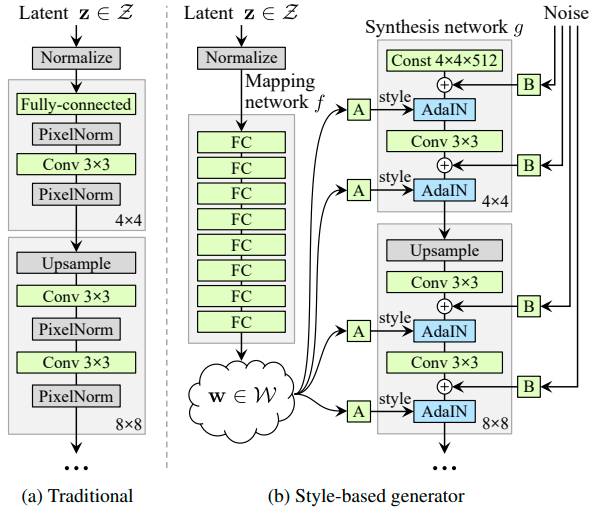
\includegraphics[width=0.8\textwidth]{obrazky-figures/struct-stylegan.png}
	\caption{Na obrázku je možné vidět porovnání tradičního generátoru (a) a stylově založeného generátoru (b), kterým je StyleGAN \cite{KarrasStyleGAN}.}
        \label{fig:stylegan}
\end{figure}

V procesu modelu StyleGAN se prvotně vstup mapuje do meziprostoru $\cal W$, který následně řídí generátor prostřednictvím AdaIN (\textit{adaptive instance normalization}) v každé konvoluční vrstvě. V dalším kroku je přidán Gaussův šum (\textit{noise}). Zde \uv{A} znamená naučenou afinní transformaci a \uv{B} aplikuje na vstupní šum naučené škálovací faktory pro každý vstupní kanál. Mapovací síť $f$ se skládá z 8 vrstev. Syntetická síť $g$ se skládá z vrstev 18 --- dvě pro každé rozlišení ($4^2$ -- $1024^2$). Výstup poslední vrstvy je převeden na RGB pomocí samostatné $1\times1$ konvoluce \cite{KarrasStyleGAN}.

Tento model se odklání od tradičního pojetí, ve kterém je latentní kód generátoru poskytován prostřednictvím vstupní vrstvy. StyleGAN využívá mapování latentního kódu $z$ pomocí mapovací sítě $f$ do latentního prostoru $\cal W$, kde jsou dále data dostupná pro každou konvoluční vrstvu. Rozdíl jde vidět na obrázku \ref{fig:stylegan}. Naučená afinní transformace poskytnutá od latentního prostoru určuje styl pro \textit{adaptive instance normalization} (AdaIN), tato operace je definování jako

\begin{equation}
    AdaIN(\textbf{x}_i, \textbf{y}) = \textbf{y}_{s,i} \frac{\textbf{x}_i - \mu(\textbf{x}_i)}{\sigma(\textbf{x}_i)}+\textbf{y}_{b,i}
    \label{eq:StyleGANAdaIN}
\end{equation}

\noindent kde $\textbf{x}_i$ je vstupní obrazový vektor a $\textbf{y}$ je vektor stylu. $\textbf{y}_{s,i}$ je skalární faktor stylu a $\textbf{y}_{b,i}$ je vektor posunu, oba pro použití v adaptivní normalizaci s $\textbf{x}_i$. $\mu(\textbf{x}_i)$ značí průměr $\textbf{x}_i$ a $\mu(\textbf{x}_i)$ směrodatnou odchylku $\textbf{x}_i$.  Každé $\textbf{x}_i$ je normalizováno samostatně a poté je škálováno na základě stylu $\textbf{y}$. V poslední řadě je generátoru poskytnut vstup šumů, pro vytvoření stochastických detailů \cite{KarrasStyleGAN}.

\bigskip

\noindent Tento model se zaměřuje na možnost modifikování stylu specifickým škálováním, která umožňuje různé zaměření na vykreslení detailů. Další vlastností je míchání stylů (\textit{style mixing}), které umožňuje spojit dva různé styly, místo jednoho. Děje se tak při změně jednoho latentního kódu na druhý v náhodně vybraném bodě sítě syntézy. Přesněji existují dva latentní kódy $\textbf{z}_1$, $\textbf{z}_2$, které odpovídají latentním prostorům $\textbf{w}_1$, $\textbf{w}_2$. Styl $\textbf{w}_1$ je aplikován až do okamžiku výměny, kde pak přebírá kontrolu styl $\textbf{w}_2$ \cite{KarrasStyleGAN}.

\begin{figure}[H]
	\centering
	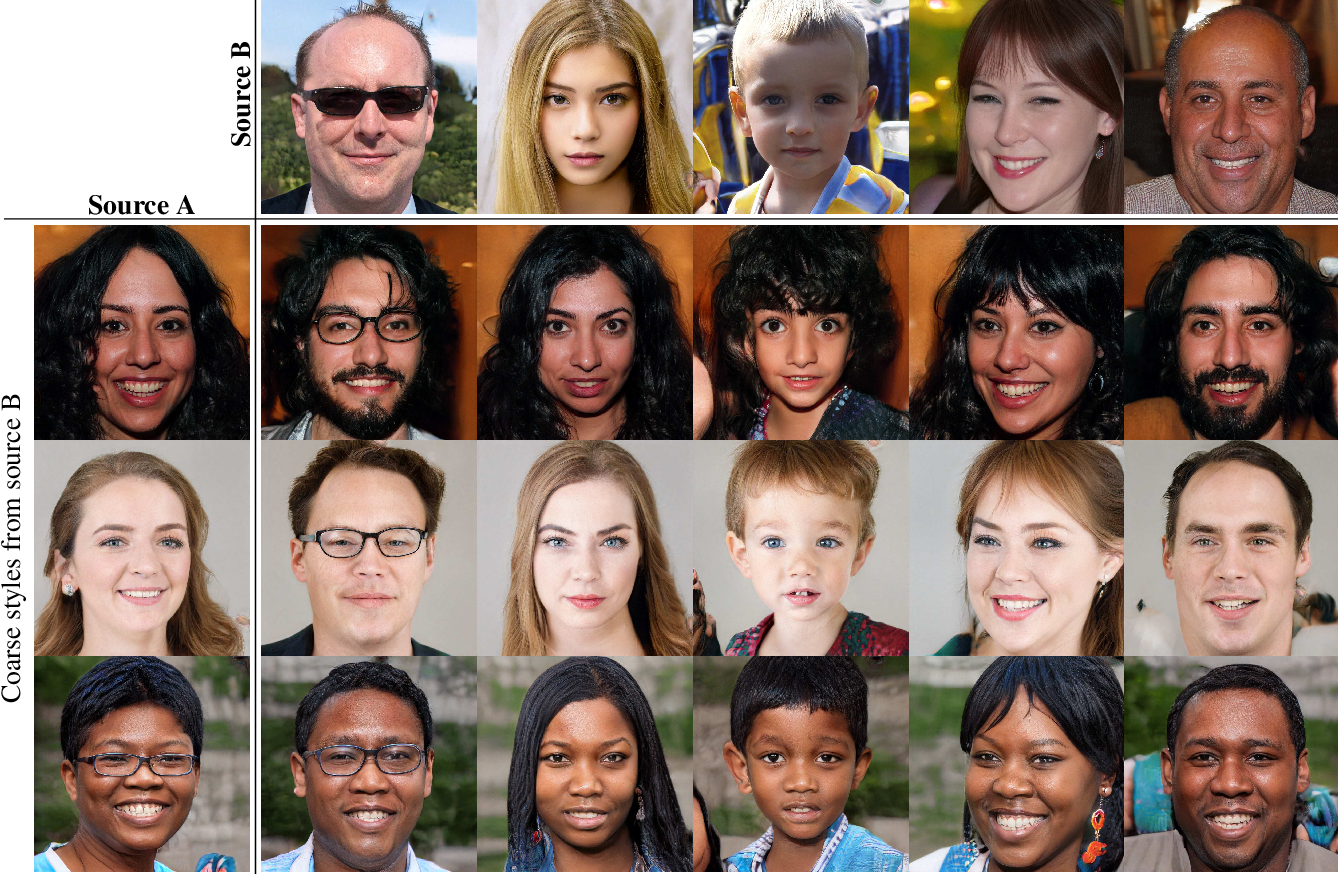
\includegraphics[width=1\textwidth]{obrazky-figures/mixing-stylegan-part.png}
	\caption{Dvě sady snímků byly vygenerovány z odpovídajících latentních kódů (\textit{Source A} a \textit{Source B}). Zbytek obrázků byl vygenerován pomocí stylu z zdroje B a následně zdroje A. Kopírování stylů odpovídající hrubému rozlišení ($4^2 - 8^2$), umožňuje přenést vlastnosti vyšší perspektivy, jako jsou póza, styl účesu, tvar obličeje a brýle, ze zdroje B a styl barev (oči, vlasy, nasvícení) je přenesen ze zdroje A \cite{KarrasStyleGAN}.}
        \label{fig:mix-stylegan}
\end{figure}

StyleGAN2 \cite{karras2020analyzing} představuje novou generaci tohoto modelu, vyvinutou s cílem eliminovat problematické oblasti, které se objevily v původní verzi StyleGAN \cite{KarrasStyleGAN}. Hlavním problémem, který byl řešen, je odstranění rušivých prvků, aby bylo dosaženo generování snímků, které jsou ještě realističtější a obtížně odlišitelné od skutečných fotografií. Jedním z těchto rušivých prvků byly artefakty připomínající vodní kapky, které vznikaly díky normalizaci instancí. StyleGAN2 proto omezuje použití adaptivní normalizace instancí s cílem odstranit tyto rušivé prvky.

StyleGAN3 \cite{karras2021alias} představuje pokračování této výzkumné práce. Na rozdíl od StyleGAN2 má několik vylepšení v síťové struktuře a v metodách tréninku. Hlavním zdokonalením je snaha zajistit, aby animace přechodů byla přirozenější, a konkrétně řeší problémy s ulpíváním textur při generování. Jedním z hlavních nedostatků vytvořených sérií snímků bylo nedostatečně realistické zobrazení vlasů a vousů. 

\subsection*{Generativní adverzní sítě tří hráčů}

GAN síť tří hráčů, přináší do minimax hry mimo generátor a diskriminátor ještě třetího člena, který se zaměřuje na identitu (ID-3 \cite{kolf2023identitydriven}), toto rozšířeni poskytuje model IDnet. Hlavním cílem modelu IDnet je problematika hry dvou hráčů při generování syntetických snímků obličeje bez oddělení identity reálných osob, která může narušovat jejich soukromí a porušovat legislativu, například při tvorbě datasetů pro trénování modelů pro rozpoznání obličeje (\textit{face recognition}). Rozšíření o třetího hráče může zajistit, že k takovým narušením nedojde a vygenerované výsledky budou oddělené od reálných identit lidí, kteří nemuseli poskytnout pro zpracování do datasetu souhlas a to se zachováním kvality výsledných obrázků.

Model IDnet funguje na architektuře dvou hráčů StyleGAN2-ADA s přidáním třetího hráče ID-3, který funguje jako model pro \textit{face recognition}, který je zaintegrován do \textit{loss function}. ID-3 je trénován pomocí \textit{softmax loss function} s penalizací za marži, která zahrnuje penalizaci za marži v softmax ztrátě, aby se trénovací vzorky přiblížily ke středům svých tříd a vzdálily se od středů ostatních tříd. Konkrétně se k tréninku ID-3 používá \textit{loss function} \textit{face recognition} modelu CosFace. Náš nový hráč má za cíl vést generátor $G$ k tomu, aby se naučil vytvářet syntetické obrazy s vysokou variabilitou a silnou oddělitelností identit \cite{kolf2023identitydriven}.

\subsection*{Zhodnocení současného stavu GAN}

Neuronové sítě a svět umělé inteligence jsou v současné době na vrcholu, kde rozvoj pokroku a inovací směřuje rychlým tempem kupředu a otevírají se nové možnosti. Konkrétně bylo nahlíženo na oblast generativních neuronových sítí, zejména sítě GAN. Tyto sítě pracují s~principem soutěže mezi generátorem a diskriminátorem, což vede k vytváření realistických a kvalitních vizuálních obsahů. Existuje mnoho rozdílných přístupů využití GAN pro různé účely, přičemž se nejvíce liší ve ztrátových funkcích. Každý z přístupů má trochu jiné vlastnosti a zpracování snímků pro editaci a tvorbu, nicméně všechny přináší kvalitu a posun ve tvorbě uměle vygenerovaných snímků obličeje. V rámci této práce se zdá nejvhodnější použít model StyleGAN, umožňující generování snímků na škále rozlišení, která přenáší na nově vygenerované snímky různé vlastnosti v závislosti na zvoleném rozlišení.

\section{Detekce antropometrických bodů v obrazu}

Důležitým aspektem pro zkoumaní a měření obličeje jedince, v oblasti počítačového vidění, jsou antropometrické body na obličeji, které umožňují význačné oblasti obličeje podrobně zkoumat.
Před jakýmkoliv zkoumáním antropometrických bodů je nejprve potřeba lokalizovat obličej, poté je možné se posunout k detekci těchto bodů. K tomu může být použita například knihovna \it OpenCV \rm pro funkce v oblasti počítačového vidění v reálném čase \cite{pyLandmarks}.

Existuje celá řada detektorů obličejových antropometrických bodů, ale všechny metody se v podstatě snaží lokalizovat a označit následující oblasti obličeje:

\begin{itemize}
    \item ústa,
    \item pravé obočí,
    \item levé obočí,
    \item pravé oko,
    \item levé oko,
    \item nos,
    \item čelist.
\end{itemize}

\noindent Knihovna dlib \cite{Kazemi2014OneMF}\cite{pyLandmarks} je jedním z možných řešení pro vyhledání antropometrických bodů na obličeji, využívá práci autora V. Kazemi a J. Sullivan (dostupná na \cite{Kazemi2014OneMF}). Tento rámec je založen na učení se sady regresních stromů pro optimalizaci součtu kvadratických ztrát a přirozeně se vypořádává s chybějícím nebo částečně označenými daty. Algoritmus manuálně označí body na obličeji, podle obecného schématu a poté zdokonaluje jejich polohu \texttt{x} a \texttt{y} souřadnic, dokud antropometrické body nejsou umístěné na správném místě. Proces je zachycen na snímku \ref{fig:casc-reg}. 

\begin{figure}[H]
	\centering
	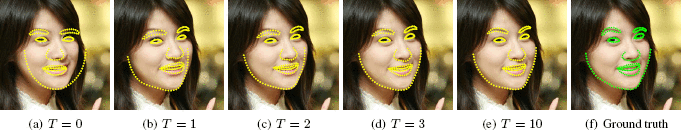
\includegraphics[width=1\textwidth]{obrazky-figures/facial-landmark-regr.png}
	\caption{Regresivní kaskáda pro určování odhadovaného rozložení antropometrických bodů na obličeji v jednotlivých stádiích. Již po první úrovni kaskády se chyba výrazně sníží \cite{Kazemi2014OneMF}.}
        \label{fig:casc-reg}
\end{figure}

S použitím datové sady (angl. \textit{dataset}) iBUG 300-W, na kterém byl dlib trénován získáme 68 souřadnic \texttt{(x,y)}, které mapují obličejové struktury na obličeji. Dataset vznikl v rámci studie: \textit{300 Faces in-the-Wild Challenge} (výzva 300 tváří v divočině), obsahuje autentické snímky z běžného života zachycené na různá zařízení. Dataset byl vytvořen seskládaní fotografií z jiných datových sad (jako HELEN, AFW, LFPW a další), včetně úplně nových snímků pro obohacení sady \cite{SAGONAS20163}. Základní anotaci datového setu lze vidět na obrázku \ref{fig:i300-annotation}.

\begin{figure}[H]
	\centering
	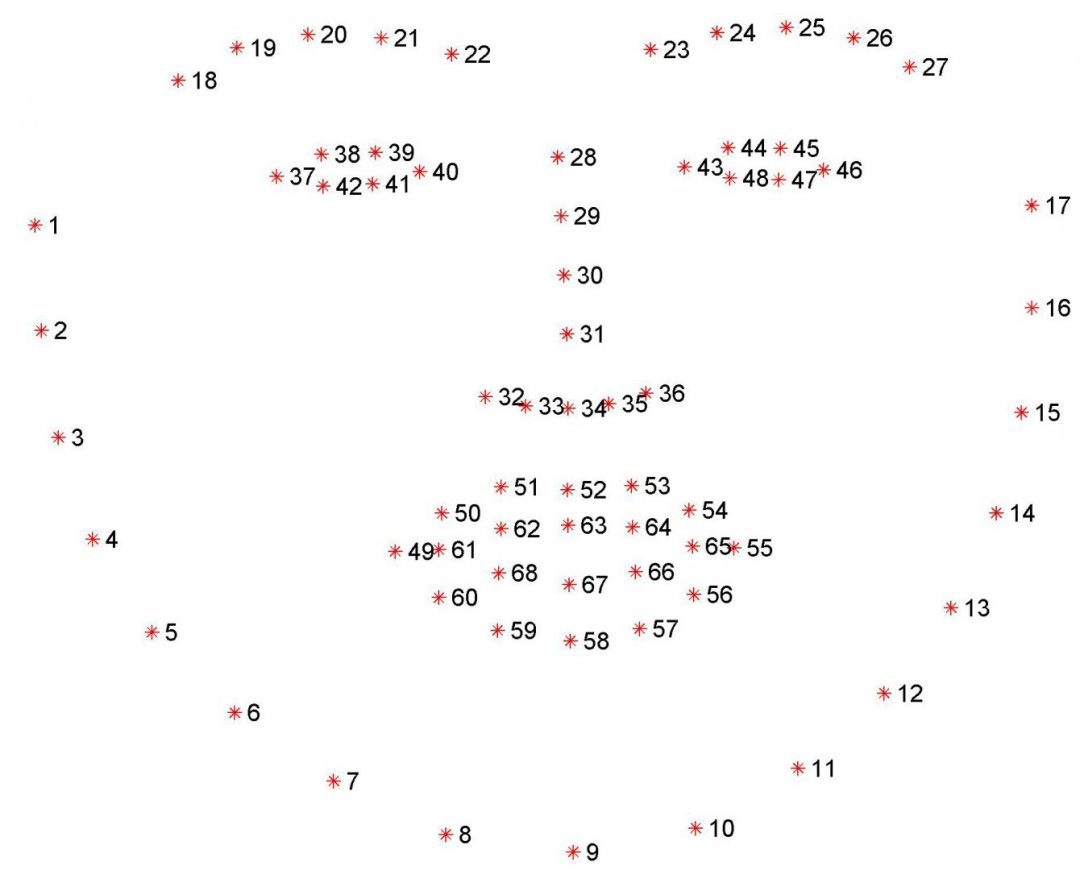
\includegraphics[width=0.7\textwidth]{obrazky-figures/i300-landmarks.jpeg}
	\caption{68 \texttt{(x,y)} souřadnic pro poskytnutí anotace datovou sadou iBUG 300-W \cite{SAGONAS20163}.}
        \label{fig:i300-annotation}
\end{figure}

\subsection*{MediaPipe}

MediaPipe \cite{lugaresi2019mediapipe} je rámec pro vytváření rour (\textit{pipeline}) pro provádění odvozování nad libovolnými smyslovými daty. Pomocí MediaPipe lze sestavit percepční \textit{pipeline} ve formě grafu modulárních komponent. Do grafu vstupují smyslová data, jako jsou zvukové a video toky, a generuje výstupní percepční popisy, jako jsou například lokalizace objektů nebo bodů obličeje. Hlavním využitím MediaPipe je rychlé vytváření prototypů percepčních \textit{pipeline} s~odvozovacími modely a dalšími opakovaně použitelnými komponentami. Díky jednoduché opakovatelnosti lze komponenty MediaPipe snadno využívat v různých \textit{pipeline} napříč po sobě jdoucími aplikacemi, protože tyto komponenty sdílejí společné rozhraní orientované na data. Každá \textit{pipeline} pak může běžet se stejným chováním na různých platformách, což umožňuje odborníkovi vyvinout aplikaci na pracovních zařízeních a následně ji nasadit například na mobilní zařízení.

MediaPipe se skládá ze tří hlavních částí: rámce pro odvozování ze senzorických dat, sady nástrojů pro hodnocení výkonnosti a sady opakovaně použitelných komponent pro odvozování a zpracování dat, tzv. kalkulátorů. \textit{Pipeline} je definována jako směrovaný graf komponent, kde každá komponenta je kalkulátor \texttt{Calculator}. V grafu jsou kalkulátory propojeny datovými toky \texttt{Streams}. Každý tok představuje časovou řadu datových paketů \texttt{Packets}. Kalkulátory a toky společně definují graf datových toků. Pakety, které protékají grafem, jsou v rámci časové řady srovnány podle svých časových značek. \texttt{Pipeline} lze postupně vylepšovat vkládáním nebo nahrazováním kalkulátorů kdekoli v grafu. Vývojáři mohou také definovat vlastní kalkulátory \cite{lugaresi2019mediapipe}.

\bigskip

\noindent Příkladem použití rámce MediaPipe je detekce objektů v reálném čase. Je například možné zpracovat výstup z videokamery a identifikovat objekty v obraze. Sledovací mechanismus (\textit{tracker}) lokalizuje polohu objektu, zatímco detektor určuje typ objektu. Pro dosažení optimálního výkonu by sledování a detekce měly probíhat paralelně, aby \textit{tracker} nebyl blokován detektorem a mohl zpracovat každý snímek.

Dalším příkladem je detekce antropometrických bodů obličeje. Proces je zde podobný jako u předchozí aplikace, provádí se detekce antropometrických bodů obličeje spolu se segmentací portrétu. Jednou ze strategií, jak snížit výpočetní zátěž potřebnou ke spuštění obou úloh současně, je použít úlohy na dvě oddělené podmnožiny snímků. Výsledná vizualizace je zobrazena jako překrytí na snímcích z kamery \cite{lugaresi2019mediapipe}.

\bigskip

\noindent Detekce antropometrických bodů v obraze je zásadním prvkem pro mnoho aplikací v oblasti počítačového vidění, zejména v analýze obličeje jedince. Zatímco knihovna dlib nabízí spolehlivé metody pro lokalizaci těchto bodů, rámec MediaPipe přináší širší perspektivu. Jeho modularita a schopnost práce s různými typy senzorických dat umožňuje rychlé prototypování a nasazení aplikací i v reálném čase. Tím se stává klíčovým nástrojem pro práci s antropometrickými body nejen v analýze obličeje, ale i v širším kontextu počítačového vidění.

\section{Rozpoznávání a ověřování obličeje}

V dnešní digitální době, kdy se technologie neustále rozvíjí, získává rozpoznávání a ověřování obličeje stále větší pozornost. Tento proces, který využívá analýzy obrazu obličeje k identifikaci jednotlivců, se stal klíčovým nástrojem v oblastech bezpečnosti, osobního identifikačního systému a uživatelské autentizace.

\bigskip

\noindent Ověřování obličeje je úloha, při níž se na základě analýzy obrazu obličeje rozhoduje, zda je daná osoba tím, za koho se vydává. Tento úkol je velmi náročný vzhledem k rozdílům v osvětlení, póze, výrazu obličeje a věku. Hlavním cílem je vypočítat \textbf{vzdálenost} \cite{CosineDistance} (\textit{distance}) mezi dvěma obličejovými vektory, což představuje míru jejich rozdílnosti.

Existuje několik metrik pro měření podobnosti, mezi nimiž se řadí eukleidovská vzdálenost, která měří vzdálenost mezi dvěma vektory, a kosinová vzdálenost, která analyzuje kosinus úhlu mezi také dvěma vektory. Oba tyto přístupy operují ve vícerozměrném prostoru~\cite{CosineDistance}.

\subsection*{Deepface}

Deepface \cite{serengil2020lightface} je odlehčený hybridní \textit{framework} pro rozpoznávání obličeje a analýzu atributů obličeje (věk, emoce, pohlaví, rasa) pro jazyk Python. Jeho hybridní přístup umožňuje přepínat mezi nejmodernějšími modely rozpoznávání obličeje, jako jsou VGG-Face, FaceNet, ArcFace, Dlib a další. Moderní postup rozpoznávání obličeje se skládá z pěti základních fází: detekce, zarovnání, normalizace, reprezentace a ověření. Deepface zvládá všechny tyto fáze na pozadí. Obrázek \ref{fig:deepface-face-detection} představuje konkrétní příklad detekce obličeje v obraze pomocí vybraných modelů v rámci Deepface.

Tento framework značně usnadňuje práci s moderními (\textit{state-of-the-art}) modely pro rozpoznávání obličeje. Uživatelé mohou jednoduše volat potřebné operace pomocí jediné funkce, které předávají specifické argumenty, jako je výběr metriky, modelu pro rozpoznávání, modelu pro detekci a dalšího nastavení. To znamená, že i uživatelé s omezenými znalostmi hlubokého učení mohou snadno využívat pokročilé technologie rozpoznávání obličeje bez nutnosti detailní znalosti fungování jednotlivých modelů a algoritmů. Kód rámce je dostupný pod licencí MIT na platformě GitHub\footnote{\url{https://github.com/serengil/deepface}}.

\begin{figure}[hbt]
	\centering
	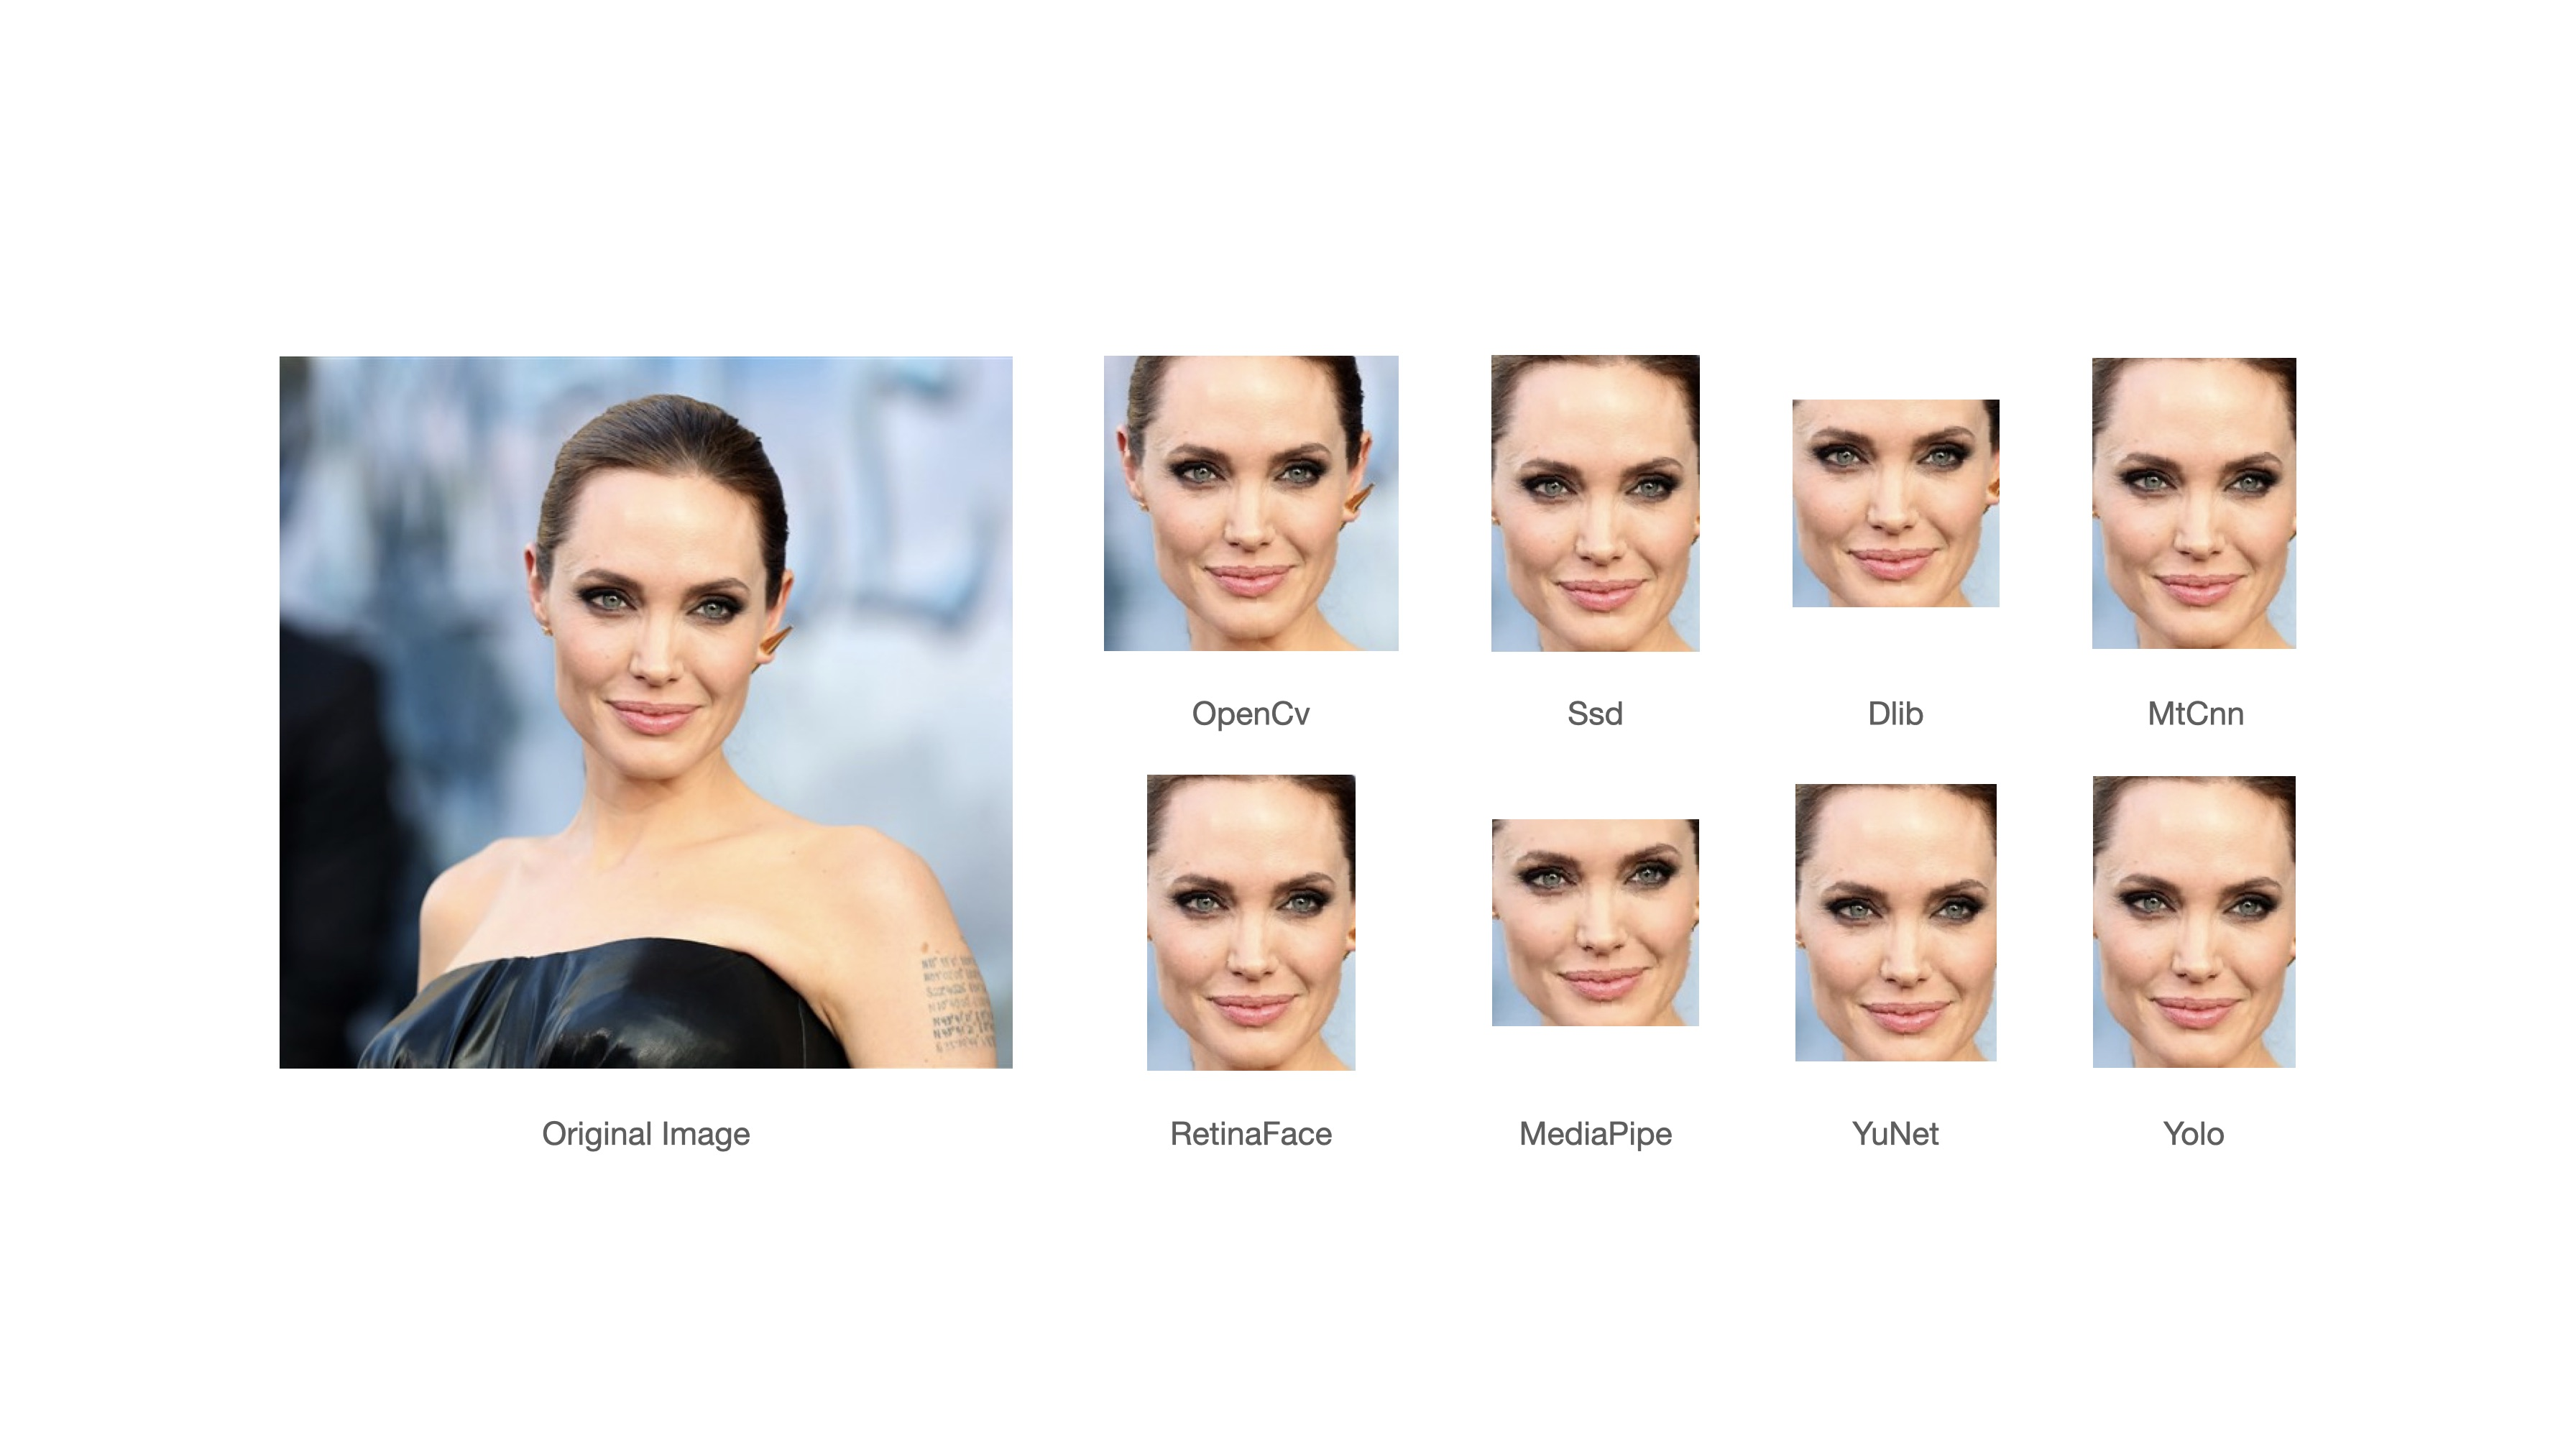
\includegraphics[width=1\textwidth]{obrazky-figures/deepface_face_detection.jpeg}
	\caption{Ukázka různých přístupů modelů využitelných v rámci Deepface k detekování lidského obličeje \cite{serengil2020lightface}.}
        \label{fig:deepface-face-detection}
\end{figure}

\subsection*{ArcFace}

ArcFace patří mezi modely vyvinuté pro řešení úkolů v oblasti rozpoznávání obličeje. Na rozdíl od jiných modelů nevyužívá přímo \textit{Softmax loss function}, ale její upravenou verzi nazvanou \textit{Additive Angular Margin Loss}. Tato úprava přináší značné výhody, jako je možnost pracovat s nečistými daty a zachovat přitom vysoký výkon. K výpočtu úhlu mezi aktuálním prvkem a cílovým středem používá funkci arkus kosinus (\textit{arccosine}). Poté k cílovému úhlu zavede \textit{additive angular margin} a pomocí kosinové funkce získá cílový logaritmus. Poté všechny logaritmy přeškáluje pevnou normou funkce. Následné kroky jsou potom prakticky totožné s postupem při využití \textit{softmax loss}. ArcFace přímo optimalizuje rozpětí geodetických vzdáleností (\textit{geodesic distance}) díky přesné korespondenci mezi úhlem a obloukem v~normalizované hypersféře. Dále je schopen pracovat s nadměrným šumem a dokáže tato tréninková data řádně vyčistit \cite{Deng_2022}.


\noindent \textit{Additive Angular Margin Loss} modelu ArcFace
\begin{equation}
    {L}=-\log\frac{e^{s\cos(\theta_{y_i}+m)}}{e^{s\cos(\theta_{y_i}+m)}+\sum_{j=1,j\neq  y_i}^{N}e^{s\cos\theta_{j}}}.
    \label{eq:arcface}
\end{equation}

kde $x_i$ je vkládaný rys, $W_{y_i}$ odpovídá třídě $y_i$, $s$ je měřítko, které reguluje velikost úhlového rozptylu, $\theta_{j}$ je úhel mezi váhou $W_j$ a rysem $x_i$, $N$ je celkový počet tříd a $m$ je úhlová penalizace mezi $W_{y_j}$ a $x_i$ \cite{Deng_2022}.

\bigskip

ArcFace je inovativním modelem pro rozpoznávání obličeje, který nepožaduje, aby datová sada obsahovala pouze čistá data. Jeho ztrátová funkce se používá k trénování neuronových sítí tak, aby vektory rysů byly lépe rozděleny v prostoru a byly lépe separovatelné podle tříd. Jeho rozšíření \textit{softmax loss function} umožňuje efektivní práci s vyšším šumem a přesto udržuje působivý výkon. Díky této schopnosti představuje ArcFace významný pokrok v oblasti rozpoznávání obličeje, který nabízí robustní řešení i pro reálné podmínky s~nečistými daty.

\begin{figure}[H]
    \centering
    \begin{subfigure}{0.45\textwidth}
         \centering
         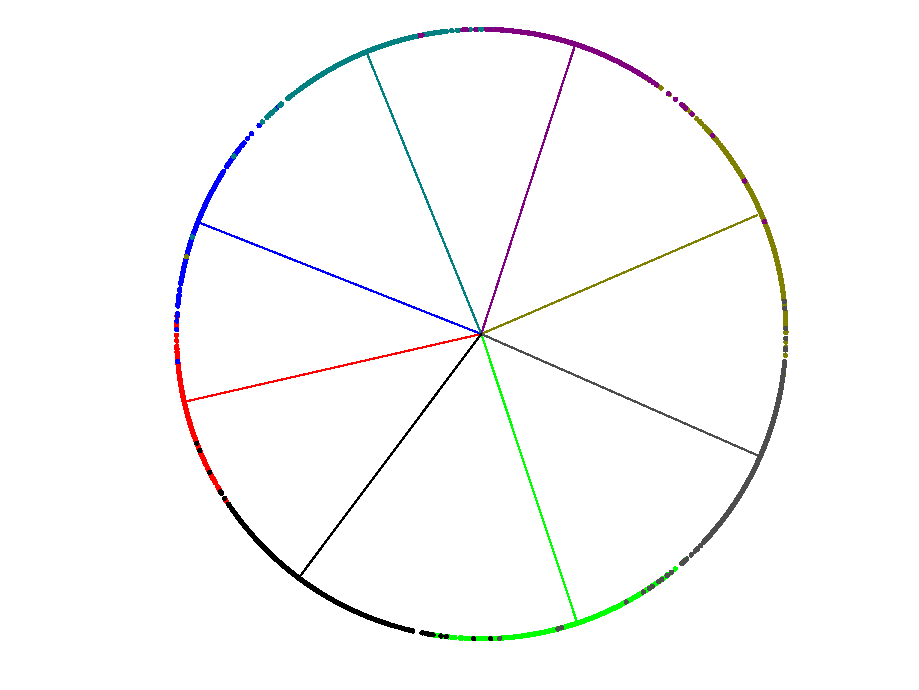
\includegraphics[width=1\textwidth]{obrazky-figures/softmaxnorm.pdf}
         \caption{Softmax}
         \label{fig:compactnesssoftmaxnorm}
     \end{subfigure}
     \hfill
     \begin{subfigure}{0.45\textwidth}
         \centering
         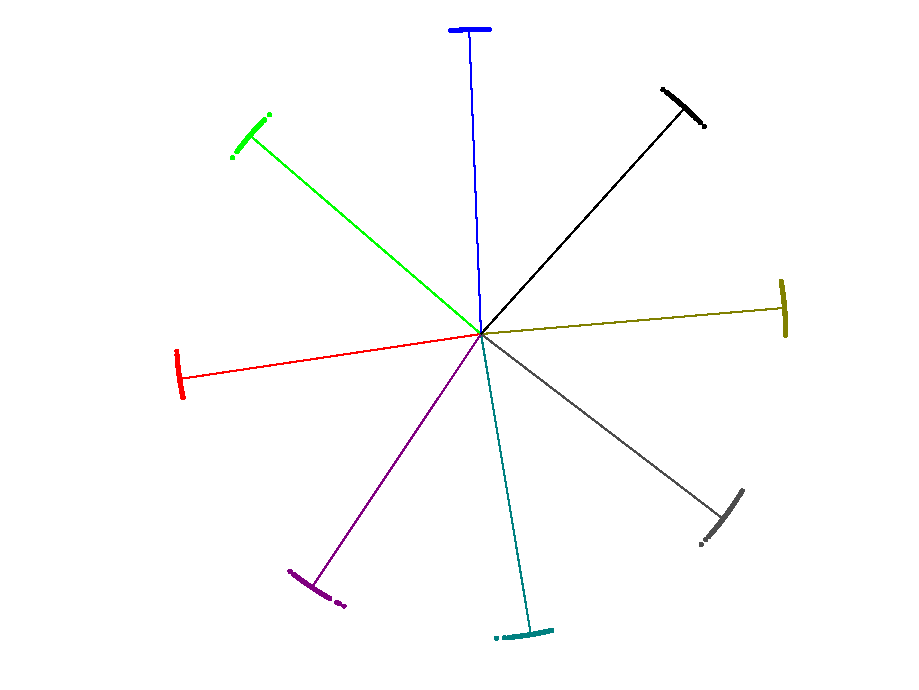
\includegraphics[width=1\textwidth]{obrazky-figures/arcfacenorm.pdf}
         \caption{ArcFace}
         \label{fig:compactnessarcfacenorm}
     \end{subfigure}
    \caption{Příklad rozdílu mezi ztrátovou funkcí (\textit{loss function}) Softmax a ArcFace na 8 různých identitách. Na základě normalizace rysů jsou všechny rysy obličeje posunuty do obloukového prostoru (\textit{the arc space}) s pevným poloměrem \cite{Deng_2022}.}
    \label{fig:compactness}
\end{figure}


\chapter{Návrh řešení a implementace analýzy antropometrických proporcí}

V této kapitole je představen návrh aplikace určené k analýze antropometrických proporcí pomocí pokročilých technologií z oblasti počítačového vidění a umělé inteligence. Hlavním cílem aplikace je posoudit rozdíly mezi uměle generovanými a reálnými snímky obličeje. Řešení aplikace spočívá v kombinaci již existujících metod umělé inteligence a vytvoření integračního systému, který umožní komplexní analýzu dané problematiky. S ohledem na spíše kombinační charakter práce a pouze částečně implementační, se na konci této kapitoly nachází i implementační detaily k jednotlivým použitým procesům.

\bigskip

\noindent Technické podrobnosti aplikace:

\begin{itemize}
    \item Operační systém: macOS 14.2
    \item Programovací jazyk a knihovny: Python 3.10
            \begin{itemize}
            \item deepface, MediaPipe, OpenCV, Matplotlib, Numpy
        \end{itemize}
\end{itemize}

\noindent Generování umělých snímků obličeje bude probíhat za pomoci modelu StyleGAN3. Vstupem pro model bude podmnožina datového setu CelebAMask-HQ o velikosti 250 snímků a výstupem budou uměle vygenerované snímky obličeje. Výsledek doplňující dvojice subsetu je základem pro další zpracování a analýzu generativních adverzních modelů. Pro provádění těchto operací jsou nezbytné následující Python knihovny: PyTorch v minimální verzi 1.9.0 a CUDA toolkit ve verzi 11.1 nebo vyšší.

\bigskip

\noindent Po získání dvojice dat -- reálných a umělých snímků, následuje jejich analýza, která se provádí ve dvou procesech.

Jeden z procesů zajišťuje vyhodnocení podobnosti na základě vzdálenosti vektorů obličeje pomocí modelu DeepFace. Druhý proces -- model MediaPipe, detekuje celkovou masku antropometrických bodů na obličeji, která se ve vyhodnocení využije pro výpočet odlišnosti u jednotlivých proporcí antropometrických bodů na obličeji.

\section{Blokové schéma návrhu}

Po seznámení s použitými technologiemi je možné se podívat na jejich propojení v rámci navrženého systému. Diagram blokového schématu je k nalezení na obrázku \ref{fig:design-diagram}.

Data ve formě podmnožiny datové sady CelebAMask-HQ, vstupují do GAN modelu StyleGAN3 pro generování umělých snímků obličeje. Každý vygenerovaný snímek je následně porovnán se svým originálním protějškem pomocí knihovny Deepface. Tento proces je analogický i pro model MediaPipe s důrazem na antropometrickou analýzu obličejů. Výsledky jsou nakonec vyhodnoceny a zobrazeny uživateli.

\begin{figure}[hbt]
	\centering
	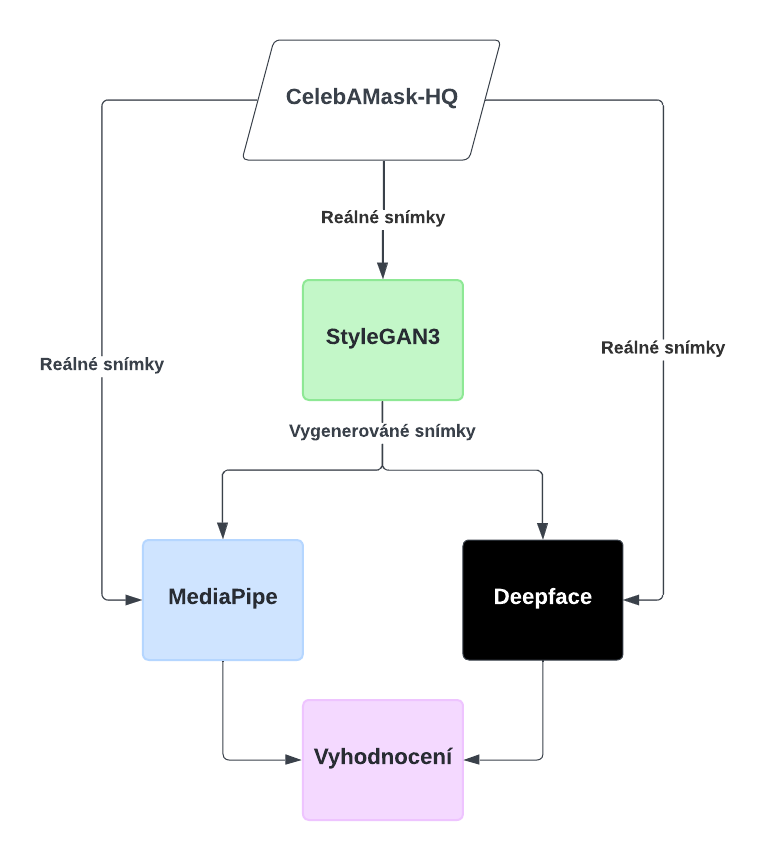
\includegraphics[width=0.75\textwidth]{obrazky-figures/design-block-diagram.png}
	\caption{Blokové schéma návrhu práce.}
        \label{fig:design-diagram}
\end{figure}

\section{Datová sada reálných snímků obličeje}


Pro generování nových snímků obličeje a jejich srovnání s původním snímkem je nutné vybrat vhodnou datovou sadu, která disponuje snímky obličeje skutečných osob. Kromě toho je vhodné z datové sady vytvořit podmnožinu dat, s cílem zlepšit kvalitu vývoje a uskutečňování experimentů.

Oblíbenou volbou je datová sada CelebA Dataset, která zahrnuje 202 599 fotografií obličejů známých osobností a obsahuje více než deset tisíc jedinečných identit. Tato komplexní datová sada je známa svou pestrostí a obsahuje obličeje s různými charakteristikami, jako jsou brýle, pokrývky hlavy, kudrnaté vlasy, knírky, vousy a variabilitou typů obličejů a dalších atributů. Dataset je příhodný pro širokou škálu aplikací, včetně rozpoznávání atributů obličeje, rozpoznávání obličeje, detekce obličeje a úpravy a syntézy obličeje. Vzhledem k~jeho nejnovější aktualizaci v roce 2021 poskytuje aktuální a rozsáhlý soubor dat \cite{CelebADataset}. 

Nicméně klasická verze CelebA datasetu může mít nízké rozlišení snímků, což nemusí vždy vyhovovat požadavkům experimentů. Proto bylo vytvořeno rozšíření od autorů původní datové sady s názvem CelebAMask-HQ Dataset, které nabízí snímky s vyšším rozlišením. Obsahuje 30 tisíc snímků vybraných z CelebA datasetu, přičemž každý z nich má rozlišení 1024x1024 pixelů, což přináší výrazné zlepšení kvality obrazu \cite{CelebAMask-HQ}. Jeho podmnožina bude využita v rámci této práce.

Pro výběr podmnožiny datové sady byla využita metoda náhodného výběru s manuální korekcí. Obsah části této podmnožiny je zobrazen na obrázku \ref{fig:CelebAMask-HQ-subset}. Tento přístup zajišťuje dostatečně velkou a reprezentativní vzorkovou množinu pro účely analýzy a experimentování.

\begin{figure}[hbt]
	\centering
	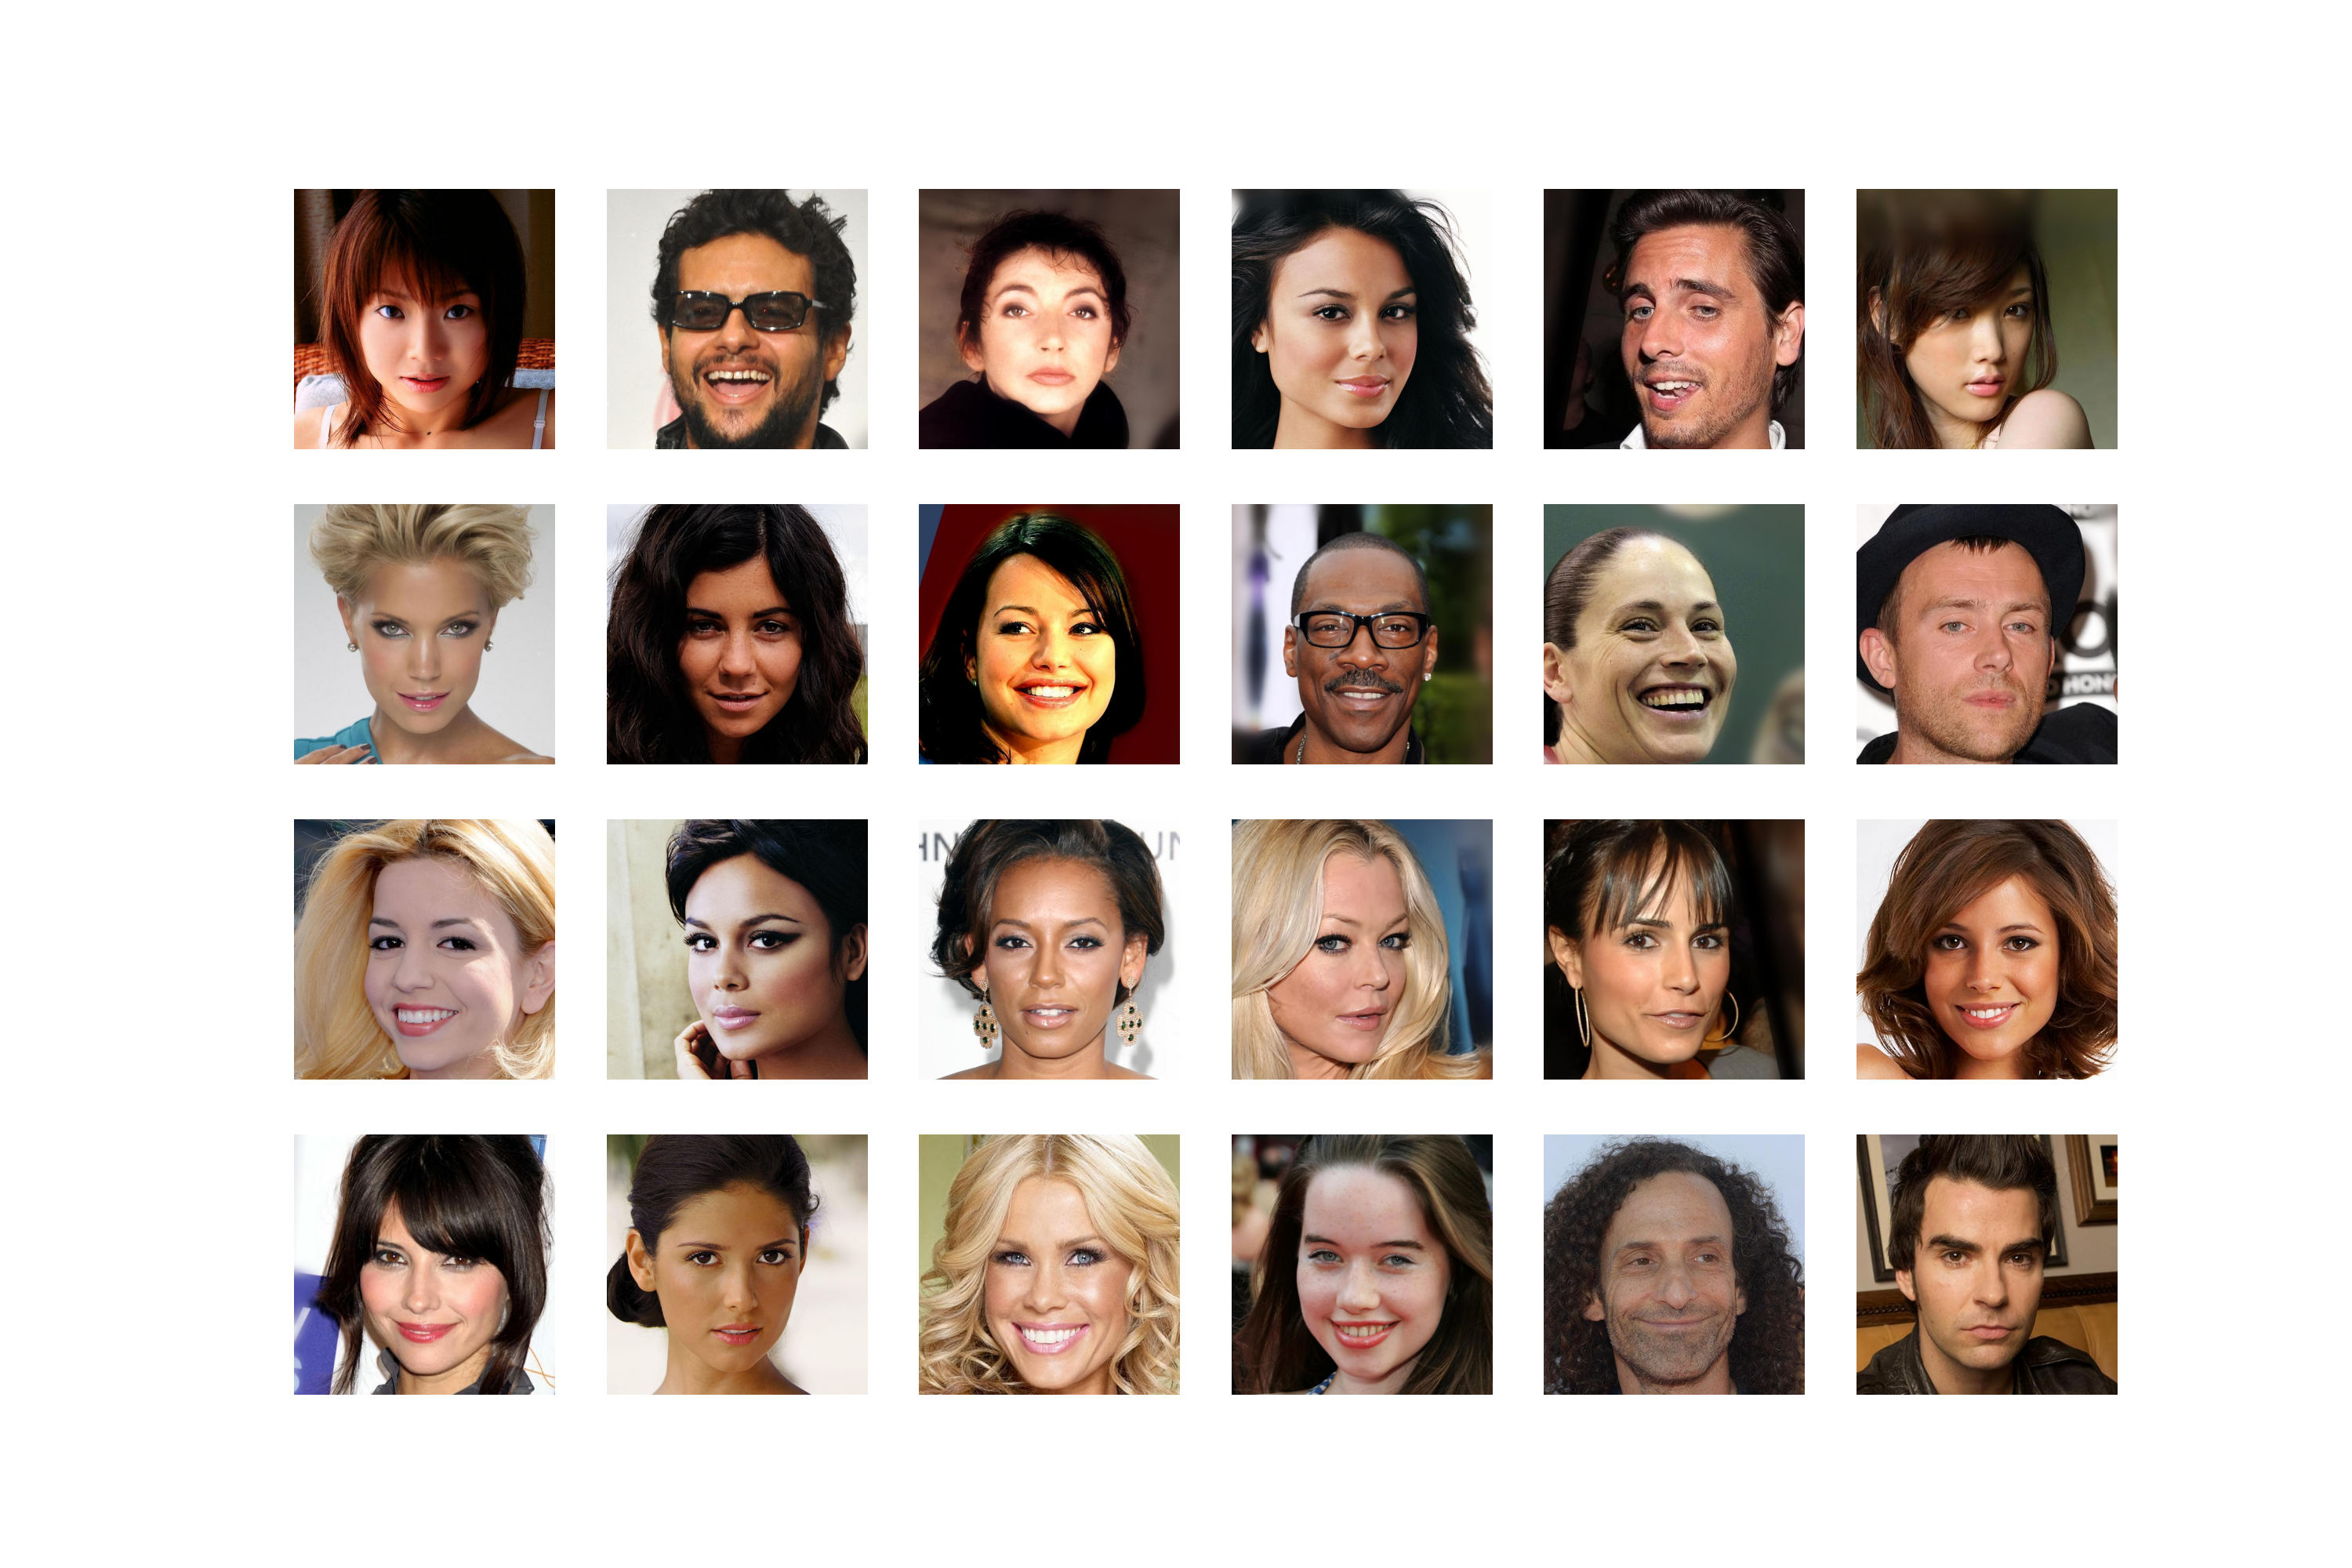
\includegraphics[width=1\textwidth]{obrazky-figures/subset-grid.png}
	\caption{Část snímků podmnožiny datové sady CelebAMask-HQ.}
        \label{fig:CelebAMask-HQ-subset}
\end{figure}

\section{Generování umělých snímků obličeje}
\label{StyleGAN-implementation}

Existuje mnoho způsobů, které dokážou generovat umělé snímky obličeje, v této práci byl zvolen model StyleGAN3 \cite{karras2021alias} od výzkumného týmu společnosti NVIDIA. Proces generování je implementován pomocí Python notebooku, který vychází z dostupných příkladů na oficiálním GitHub repozitáři modelu\footnote{Oficiální repozitář modelu: \url{https://github.com/NVlabs/stylegan3}}. Tento notebook byl dále upraven o možnost vkládání vlastních snímků a následné generování, a to díky rozšířené verzi vyvinuté výzkumníkem Eugeniem Herrera-Bergem, která je dostupná na jeho GitHub repozitáři\footnote{Rozšířená verze: \url{https://github.com/ouhenio/stylegan3-projector}}.

Použitý kód původně pochází od tvůrců a byl rozšířen o další funkce autorem Eugeniem Herrera-Bergou. Pro tuto práci byl notebook rozšířen o další funkce pro lepší použitelnost. Změnily se způsoby zpracování vstupu, kde množství fotografií obličeje není omezeno na jednu, ale uživatel může specifikovat vlastní počet fotografií. Po zpracování každé fotografie je generován umělý snímek pomocí modelu StyleGAN3, a tento proces je prováděn ve smyčce pro všechny zvolené snímky.

Kód v jazyce Python je k dispozici v souboru \texttt{StyleGAN3\_Generate\_images.ipynb}, přičemž samotné generování probíhalo na serverech Google Colab z důvodu náročnosti výpočtu a vyhnutí se problému s použitými knihovnami při spuštění lokálně. Výsledek generování spolu s původním snímkem je zobrazen na obrázku \ref{fig:stylegan3-real-and-gen-image}.

Hlavní viditelný rozdíl ve spektru všech vygenerovaných fotografií spočívá především ve výrazném rozostření pozadí a celkovém odstranění vjemů mimo obličej. Zároveň platí, že čím vyšší je kvalita původních snímků, tím méně se na výsledném obraze objevuje artefaktů a obličej působí reálněji.

\begin{figure}[H]
    \centering
    \begin{subfigure}{0.45\textwidth}
         \centering
         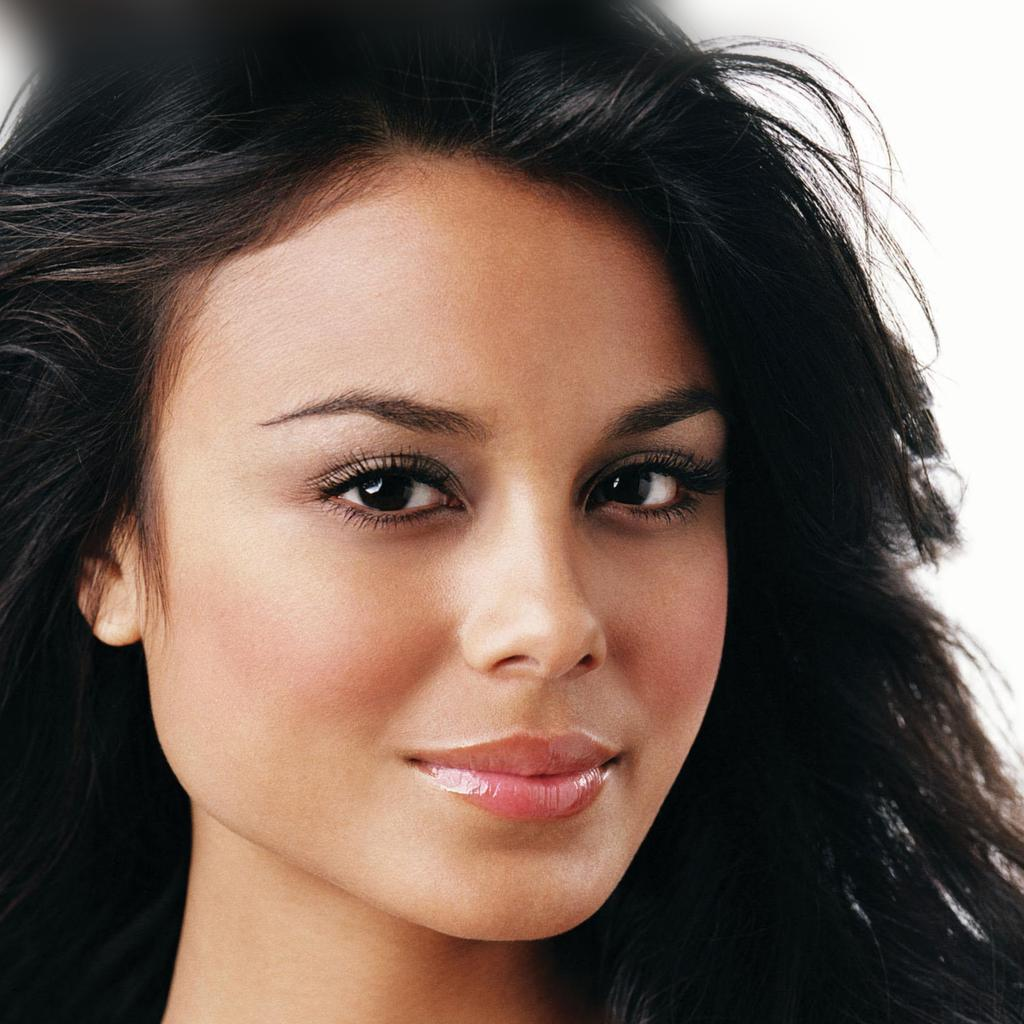
\includegraphics[width=1\textwidth]{obrazky-figures/stylegan3-real-image.jpg}
         \caption{Původní snímek obličeje}
         \label{fig:stylegan3-real-image}
     \end{subfigure}
     \hfill
     \begin{subfigure}{0.45\textwidth}
         \centering
         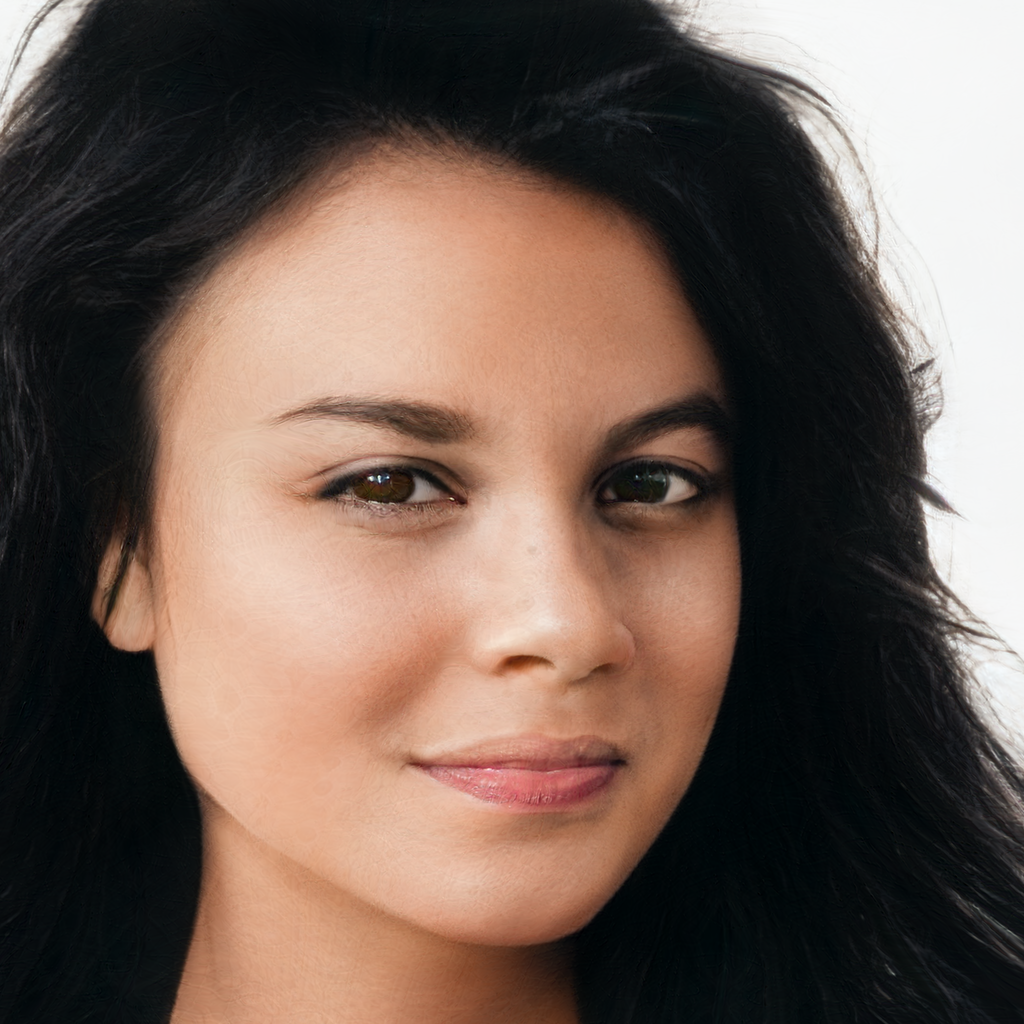
\includegraphics[width=1\textwidth]{obrazky-figures/stylegan3-gen-image.png}
         \caption{Umělý vygenerovaný snímek obličeje}
         \label{fig:stylegan3-gen-image}
     \end{subfigure}
    \caption{Porovnání reálného a vygenerovaného snímku obličeje modelem StyleGAN3.}
    \label{fig:stylegan3-real-and-gen-image}
\end{figure}

\noindent Na začátku v prvním bloku, notebook stáhne všechny nutné závislosti, definuje používané funkce (například pro stažení fotografe) a inicializuje proměnné. V dalším bloku je možné zvolit předtrénovaný model z nabídky modelů. Pro práci je použit model trénovaný na datové sadě Flickr-Faces-HQ \cite{KarrasStyleGAN}, což je vysoce kvalitní datová sada snímků lidských tváří, která byla původně vytvořena jako referenční soubor pro generativní adverzní sítě.

V dalším bloku je potřeba provést úpravy v parametrech jako je počet kroků (\texttt{steps}), počáteční hodnota \textit{seed} (\texttt{seed}) a velikost podmnožiny (\texttt{subset\_size}), se kterou se bude pracovat. Proměnná \texttt{steps} určuje počet kroků, které se provedou při procesu generování obrázků. V kontextu kódu se jedná o počet iterací, které algoritmus provede při projekci vektoru do prostoru obrázků. Čím vyšší hodnota \texttt{steps}, tím déle algoritmus trvá, a tím více se model může přizpůsobit cílovému obrázku. Pro generování snímků byla zvolena hodnota \textbf{250} kroků. Dále jsou definovány transformace obrazu pomocí knihovny TorchVision (\texttt{tf}), která zahrnuje změnu velikosti na 1024x1024 pixelů a normalizaci obrazu do rozsahu [0, 1]. Funkce \texttt{run} je definována pro provádění samotného procesu generování obrazků. Nejprve se inicializuje náhodný \textit{seed} pro PyTorch a získají se cílové rysy (\texttt{target\_features}) pro projekci. Následně se provede samotná projekce, která se skládá z několika iterací. V~každé iteraci se vygeneruje několik obrázků, vypočítá se ztrátová funkce (\texttt{loss}) a vybere se ten obrázek, který minimalizuje tuto ztrátu. Nakonec se aktualizuje váha (\texttt{q}) pomocí optimalizačního algoritmu AdamW. Po dokončení se obrázek zobrazí.

Poslední blok inicializuje cílové obrázky pro projekci. Jsou načteny obrázky ze zadaných URL adres a upraveny do požadované podoby. Poté je spuštěna funkce \texttt{run} pro každý cílový obrázek.

\begin{figure}[hbt]
	\centering
	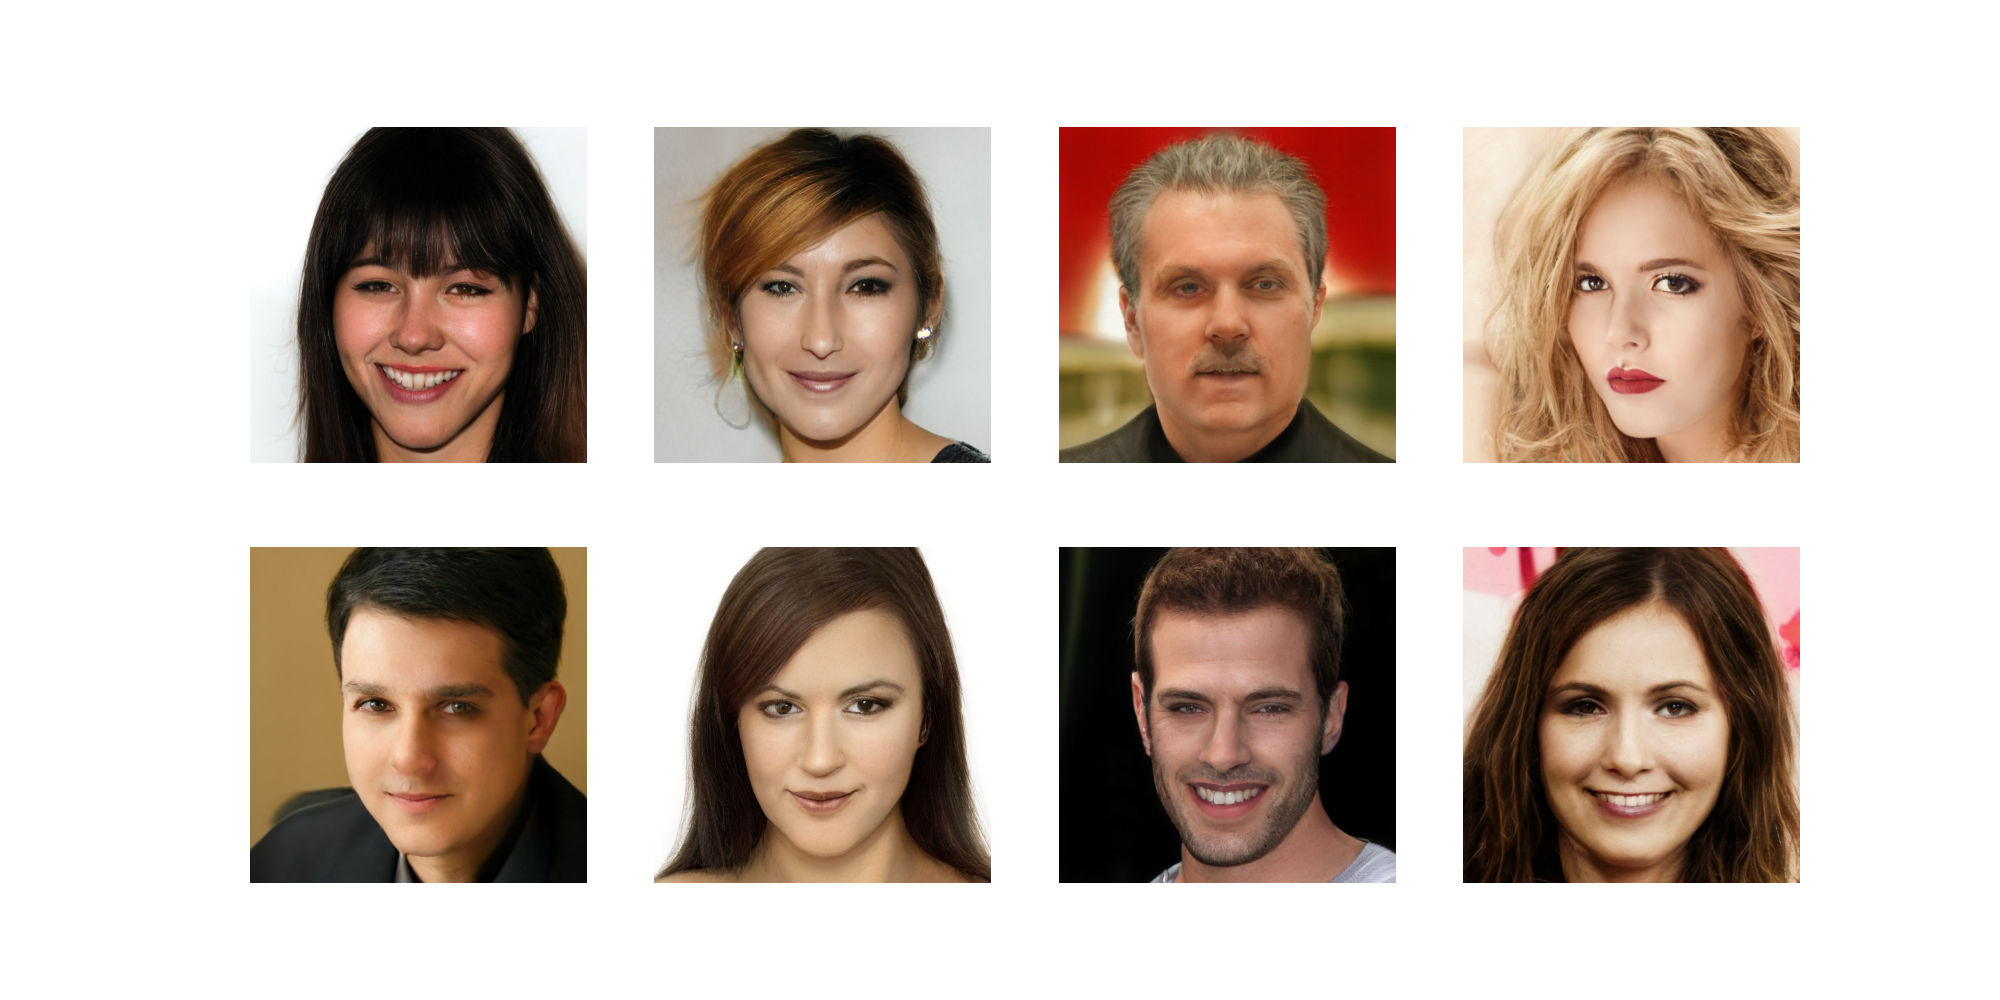
\includegraphics[width=1\textwidth]{obrazky-figures/gen-images-grid.png}
	\caption{Ukázka vygenerovaných snímků obličeje pomocí modelu StyleGAN3.}
        \label{fig:stylegan3-generated-examples}
\end{figure}

\noindent Výsledkem této sekce jsou uměle vygenerované snímky, které vytvářejí dvojice s původními reálnými snímky. Tato fáze je klíčová pro následnou analýzu, během níž jsou tyto dvojice porovnávány. Aby se zajistila lepší kvalita výsledného snímku, byly některé z vygenerovaných snímků s viditelně nízkou kvalitou přegenerovány.

\section{Informace o antropometrických bodech na obličeji}
\label{landmark-info}

Tento pomocný soubor s názvem \texttt{landmark\_info.py} obsahuje zásadní informace pro antropometrickou analýzu provedenou pomocí modelu MediaPipe, která je popsána v sekci \ref{MediaPipe-implementation}. Definuje nezbytné hodnoty, spojení a datové třídy.

Většina bodů uvedených v tabulce \ref{tab:landmarks} je pomocí konstant mapována na indexy jednotlivých bodů na masce obličeje modelu MediaPipe, přičemž bylo vycházeno z popisné fotografie na úložišti Google API pro MediaPipe\footnote{Dostupné na úložišti Google: \url{https://storage.googleapis.com/mediapipe-assets/documentation/mediapipe_face_landmark_fullsize.png}}, která obsahuje popis všech indexů na vykreslených bodech.

Tyto body, které je možné viděl na obrázku \ref{fig:draw-face-landmarks}, jsou propojovány pomocí datové třídy \texttt{LandmarkMeasurements}. Třída obsahuje atributy, kde \texttt{start} zastupuje počáteční bod měření, \texttt{end} zastupuje koncový bod a \texttt{name} představuje název měření. Jednotlivé instance tříd představují konkrétní měření na obličeji a jsou uchovány v konstantě \texttt{FACE\_PROPORTIONS}, která vytváří seznam těchto vybraných měření. Měření pro analýzu obličeje tvoří podmnožinu měření ze sekce \ref{facial-landmarks} a jsou následující:

\begin{itemize}
    \item měření obličeje -- šířka obličeje (zy-zy), šířka čelisti (go-go), výška dolní části obličeje (sn-gn), výška obličeje (tr-gn), výška obličeje (n-gn), výška horní části obličeje (n-sto), výška dolní třetiny obličeje (sto-gn), speciální výška obličeje vlevo (en-gn), speciální výška obličeje vpravo (en-gn), speciální výška horní části obličeje (g-sn)
    \item měření orbitu -- šířka mezi oči vnější (ex-ex), šířka mezi oči vnitřní (en-en), šířka levého oka (ex-en), šířka pravého oka (ex-en)
    \item měření nosu -- šířka nosu (al-al), výška nosu (n-sn)
    \item měření úst -- šířka úst (ch-ch), výška horního rtu (ls-sto), výška dolního rtu (sto-li)
\end{itemize}

\noindent Další implementovanou třídou je datová třída \texttt{MaxDifference}, která má atributy \texttt{value}, který značí součet všech hodnot jednoho typu měření, a \texttt{count}, který představuje počet výskytů tohoto typu. Při každém porovnání dvojic je přidán pouze ten typ měření, který dosáhl nejvyšší hodnoty.

\begin{figure}[H]
	\centering
	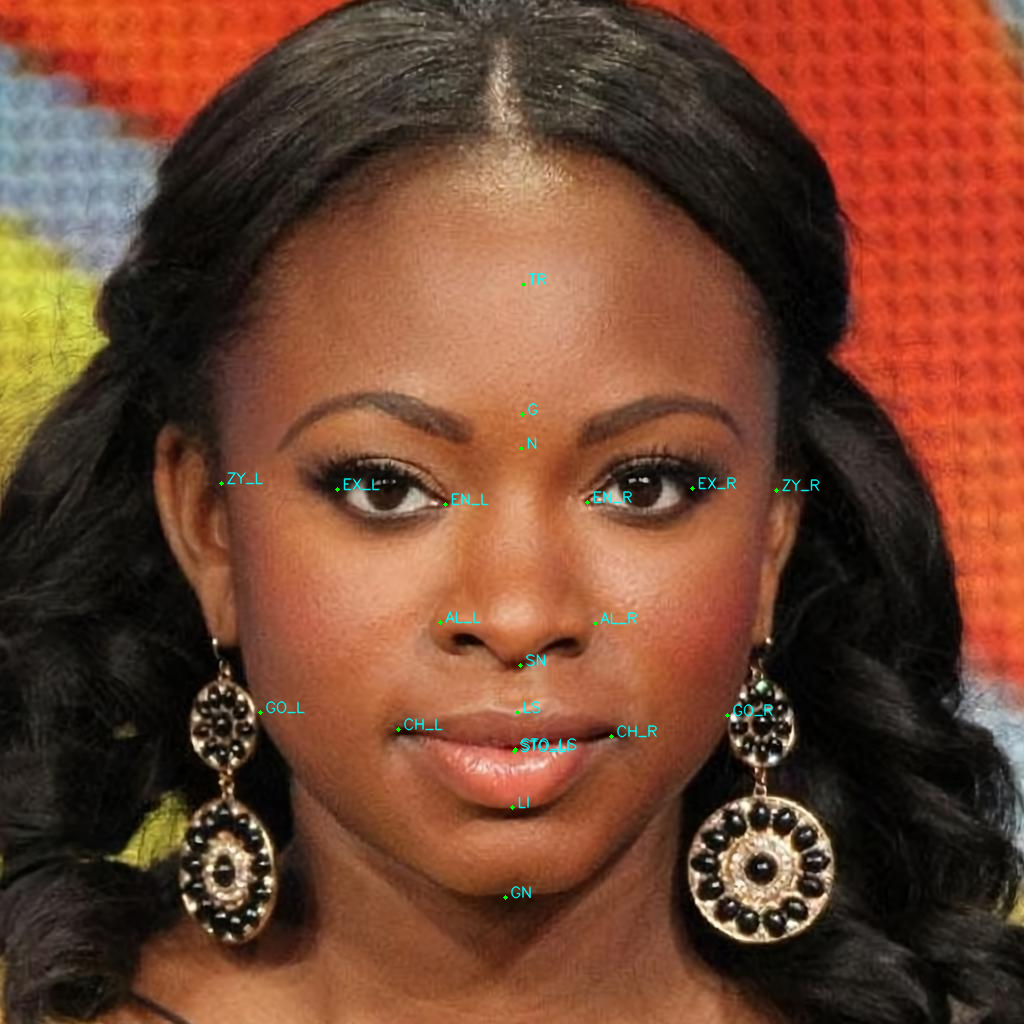
\includegraphics[width=0.75\textwidth]{obrazky-figures/landmarks_points_names.png}
	\caption{Vybrané zkoumané antropometrické body na obličeji. Názvy bodů jsou konstanty s hodnotou odpovídající indexu na masce modelu MediaPipe.}
        \label{fig:draw-face-landmarks}
\end{figure}

\noindent Druhý seznam obsahující hodnoty morfologické šířky a výšky obličeje je uložen v konstantě \texttt{TFI} pro výpočet poměru TFI. Pracuje stále s datovou třídou \texttt{LandmarkMeasurements}, ale na rozdíl od předchozí konstanty je její velikost omezena na dvě zmíněná spojení.


\section{Antropometrická analýza významných bodů obličeje}
\label{MediaPipe-implementation}

V této první části analýzy se program zaměřuje na podrobné měření poměrů mezi antropometrickými body na obličeji. Poměry a významné body vychází z antropometrické analýzy provedené v Řecku \cite{Zacharopoulos2016}, více informací se nachází v sekci \ref{facial-landmarks}. Pro zpracování a získání klíčových bodů na obličeji je využit model MediaPipe a jeho knihovny. Konkrétně využíváme předtrénovaný model \texttt{face\_landmarker\_v2\_with\_blendshapes.task}, který slouží jako vstup pro inicializační volbu modelu. Tento model umožňuje detekci klíčových bodů na snímcích obličeje. Z těchto a dalších možností vytváříme objekt \texttt{detector}, který slouží k detekci klíčových bodů na snímcích obličeje. Při lokalizaci významných bodů je nutné počítat s tím, že může dojít k nepřesnému či chybnému určení některého z bodů. Grafický výsledek detekce klíčových bodů na obličeji je na obrázku \ref{fig:facemesh-mediapipe}, kde je zobrazena celá maska klíčových bodů překrytých přes původní snímek obličeje.

\begin{figure}[H]
	\centering
	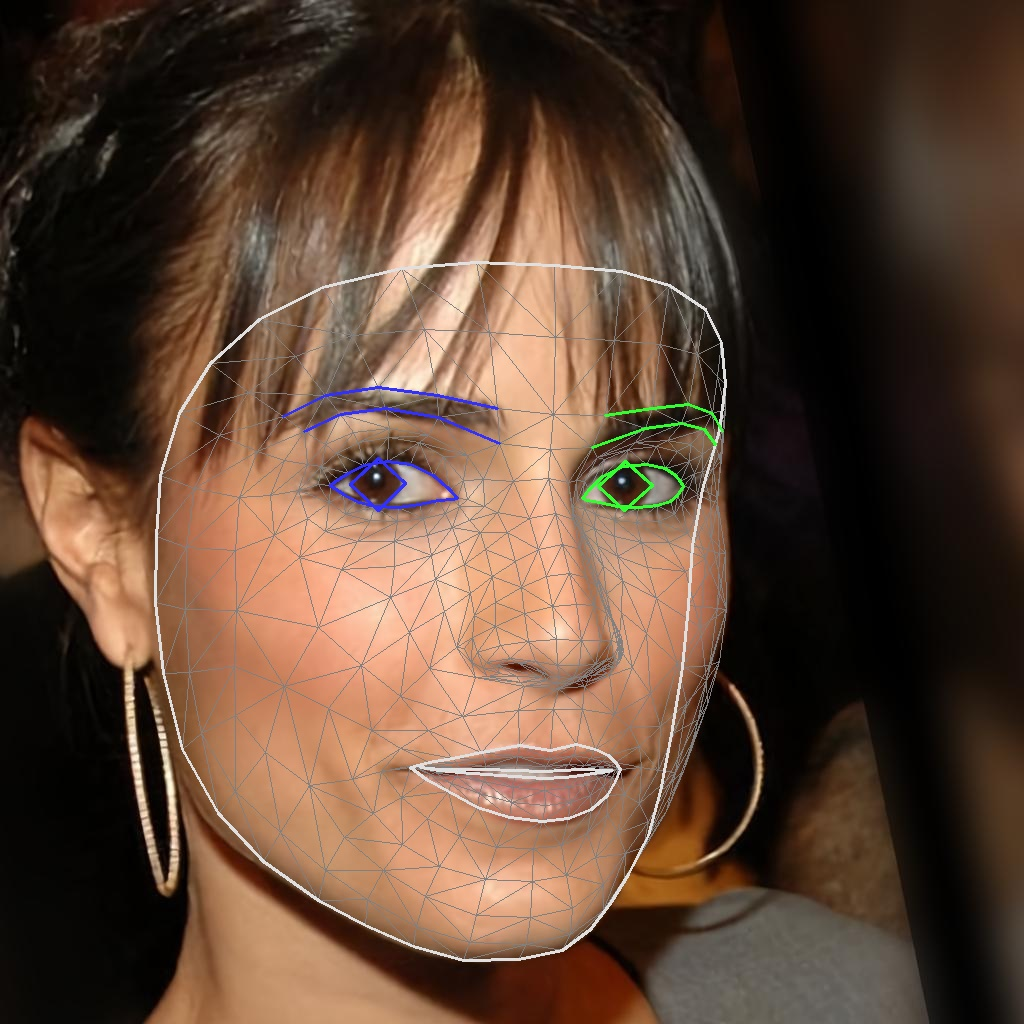
\includegraphics[width=0.8\textwidth]{obrazky-figures/mediapipe_landmarks.jpg}
	\caption{Ukázka vizualizace výsledků detekce antropometrických bodů obličeje modelu MediaPipe.}
        \label{fig:facemesh-mediapipe}
\end{figure}

Před detekcí antropometrických bodů na jednotlivých snímcích je nezbytné snímky získat. Slouží k tomu primárně dvě pomocné funkce popsané v sekci \ref{helpers} pro práci se soubory a adresáři. První z nich seřadí soubory v adresáři a druhá funkce následně získá absolutní cesty pro každý obrázek k dalšímu zpracování, pokud je vstupem programu pouze jedna dvojice snímků, nedochází k seřazení a je navrácena pouze absolutní cesta snímků. Poté již dochází k detekování bodů na obličeji pomocí detektoru \texttt{detector} a uložení výsledků do proměnný, pro každou skupinu, reálných a generovaných snímků, zvlášť.

Další proces spočívá v měření jednotlivých poměrů, které jsou uložené jako seznam v~konstantě \texttt{FACE\_PROPORTIONS}, která je získána z pomocného souboru \texttt{landmark\_info.py}, který je více popsaný v sekci \ref{landmark-info}. Pro každé měření je spočítána vzdálenost dvou bodů v trojrozměrném prostoru (MediaPipe poskytuje pro každý bod tři souřadnice \texttt{x}, \texttt{y} a \texttt{z}). Výpočet vzdálenosti probíhá ve funkci \texttt{calculate\_distances} a je založen na eukleidovské vzdálenosti vyjádřené vzorcem

\begin{equation}
    distance = \sqrt{(x_2 - x_1)^2 + (y_2 - y_1)^2 + (z_2 - z_1)^2}
\end{equation}

kde $distance$ značí vypočítanou vzdálenost a $x_1$, $y_1$ a $z_1$ jsou souřadnice jednoho bodu a $x_2$, $y_2$ a $z_2$ bodu druhého.

Funkce, která provádí celý tento proces, nese název \texttt{measure\_face\_proportions}. Vrací slovník vzdáleností, kde je klíčem název měření a hodnotou je naměřená vzdálenost.

\bigskip

\noindent Získání hodnot vzdáleností z reálných a generovaných snímků je porovnáno pomocí funkce \texttt{compare\_proportions}, kde se vypočítává rozdíl pro každou dvojici klíčů. Nad všemi absolutními hodnotami porovnání je vypočítán průměr uložený do \texttt{avg\_diff}.

Program dále pokračuje funkcí \texttt{max\_absolute\_proportion\_difference}, která provádí analýzu poměrů s největším rozdílem vzdálenosti, tedy těch měření, u kterých se proporce nejvíce liší. Prochází všechny hodnoty výsledku srovnání a vybírá tu, který má nejvyšší absolutní hodnotu, tedy i největší rozdíl ve vzdálenosti. Hodnoty jsou uloženy pro další rozbor v rámci experimentů.

\bigskip

\noindent Paralelně jsou získány hodnoty potřebné k výpočtu hodnoty celkového indexu obličeje (TFI). Potřebná je šířka a výška obličeje, pro přístup k těmto proporcím slouží konstanta \texttt{TFI}. Hodnoty jsou získány pomocí funkce \texttt{calculate\_distances} a jsou uloženy do příslušných seznamů a je vypočítána hodnota TFI pomocí funkce \texttt{calculate\_TFI}, také uložená do příslušného seznamu (\texttt{real\_tfi} nebo \texttt{gen\_tfi}). Při jakékoliv rotaci obličeje může dojít ke zkreslení

\section{Porovnání uměle vygenerovaných a reálných snímků obličeje}
\label{Deepface-implementation}

Druhým blokem pro vyhodnocení rozdílnosti mezi generovanými a reálnými snímky je využití odlehčeného (\textit{lightweight}) rámce \textbf{Deepface} \cite{serengil2020lightface}. Tento rámec poskytuje širokou škálu funkcí, které umožňují přesné srovnání obličejů a analýzu jejich podobnosti, využívá knihovnu \texttt{tensorflow}. Jeho použití umožňuje přímočaré využití konkrétních funkcí s možností volby téměř libovolného modelu pro vykonání úlohy.

Program pracuje se dvěma adresáři obsahujícími reálné a generované snímky, stejně jako bylo popsáno v sekci \ref{MediaPipe-implementation}. Každá dvojice snímků je následně porovnána pomocí vestavěné funkce rámce Deepface. Konkrétně se jedná o funkci pro ověřování obličejů \texttt{verify()}, která slouží k ověřování snímků obličeje. Pro rozpoznávání obličeje je použit model ArcFace, který je známý svou vysokou přesností a robustností. Pro detekci obličeje je využíván detektor retinaface (odlišnost detektorů je na obrázku \ref{fig:deepface-face-detection}). Pro metriku měření podobnosti byla zvolena kosinová vzdálenost jako výchozí hodnota funkce.

\bigskip

\noindent Samotné volání funkce vypadá následovně

\begin{lstlisting}[language=Python]
    result = DeepFace.verify(real_image_path, gen_image_path,
                                model_name="ArcFace",
                                detector_backend='retinaface')
\end{lstlisting}

kde výsledek porovnání \texttt{result} poskytuje informace o podobnosti mezi obličeji na snímcích, což umožňuje detailní analýzu rozdílů mezi generovanými a reálnými obličeji. Pro program jsou zásadní následující informace z výsledku:

\begin{itemize}
    \item \texttt{verified} (ověřeno) -- hodnota vyjadřující, jestli se v porovnání jedná o stejnou osobu (\texttt{True}) nebo nikoliv (\texttt{False})
    \item \texttt{distance} (vzdálenost) -- hodnota vzdálenosti mezi vektory obličeje, čím nižší hodnota vzdálenosti, tím větší podobnost mezi obličejovými rysy
    \item \texttt{max\_threshold\_to\_verify} (prahová hodnota ověření) -- maximální hodnota vzdálenosti pro vyhodnocení stejné identity
\end{itemize}

\noindent Pro prezentaci výsledků je využívána knihovna \texttt{matplotlib.pyplot}, která umožňuje vizualizaci dat prostřednictvím grafů. Jedním z grafických vyobrazení výsledků je \textbf{kruhový diagram} (angl. \textit{pie chart}). Zobrazuje procentuální úspěšnost porovnání obličejů s výsečemi úspěch a neúspěch. Druhým typem grafu využívaným k prezentaci výsledků je \textbf{korelační diagram} (angl. \textit{scatter plot}). Zobrazuje jednotlivé hodnoty vektorů vzdálenosti pro každou z dvojic. Vykreslena je i prahová hodnota (\textit{threshold}) pro určení úspěšnosti.

\section{Pomocné skripty a funkce}
\label{helpers}

Tato sekce popisuje skripty a funkce, které pomáhají s některými procesy při tvorbě této práce. Všechny uvedené funkce a příslušné soubory jsou uloženy v adresáři \texttt{helpers}, který slouží jako úložiště pro pomocné nástroje a funkce používané v rámci projektu.

\subsection*{Vytvoření podmnožiny datové sady}

Použitý dataset je pro tento typ práce moc velký, proto je nutné využít jeho podmnožinu. Získání této podmnožiny probíhá stochastickým výběrem napříč celým datasetem dokud není dosaženo požadované velikosti podmnožiny. Tento postup umožňuje získat reprezentativní vzorek dat pro daný úkol. Implementované funkce se nachází v souboru \texttt{create\_subset.py}.

Několik implementovaných pomocných funkcí slouží k manipulaci se soubory mateřského datasetu. Hlavní funkce je \texttt{copy\_random\_images}, která kopíruje náhodné obrázky z~daného zdroje do cílového adresáře. Pokud je zdrojem zip soubor, nejprve je extrahován do dočasného adresáře a poté jsou z něj vybrány náhodné obrázky ke kopírování. Tento proces vykonává funkce \texttt{extract\_zip\_to\_temp}, která slouží k extrakci obsahu zip souboru do dočasného adresáře. Ve funkci \texttt{parse\_arguments\_create\_subset} jsou zpracovány argumenty příkazové řádky a volá se hlavní funkce \texttt{copy\_random\_images} s nimi.

\subsection*{Zobrazení podmnožiny datové sady jako obrázek}

Pomocná funkce pro vytvoření obrázku ve stylu mřížky pro zobrazení všech položek v podmnožině datové sady v daném adresáři. Obrázek se využívá jako ukázka subsetu pro přiložení do textu práce. Implementované funkce se nachází v souboru \texttt{grid\_image\_subset.py}.

Po zavolání hlavní funkce \texttt{create\_grid\_image} se nejprve přes funkci \texttt{load\_images} načtou obrázky z daného adresáře, přičemž akceptují se pouze soubory s příponami JPG, PNG a JPEG. Následně funkce \texttt{create\_subplot\_grid} vytváří mřížku obrázků z načtených obrázků, která se používá k vizualizaci. Nakonec je zde funkce \texttt{save\_subplot\_grid}, která ukládá vytvořenou mřížku obrázků do souboru. Snímky jsou seřazeny.

\subsection*{Vykreslení antropometrických bodů na snímek obličeje}

Tato pomocná funkce slouží pro vizualizaci výsledků detekce antropometrických bodů obličeje modelu MediaPipe \cite{mediapipe}. Část zdrojového kódu byla převzata od autorů MediaPipe a je licencována pod Apache License 2.0\footnote{\url{https://www.apache.org/licenses/LICENSE-2.0}}.

První funkce, která načítá model MediaPipe a provádí detekci významných bodů na obličeji, nese název \texttt{get\_image\_with\_landmarks}. Další částí je načtení snímku obličeje a po úspěšné operaci také uložení anotovaného obrázku. Tato funkce rovněž volá funkci \texttt{draw\_landmarks\_on\_image}, která se stará o vizualizaci detekované mapy antropometrických bodů a vrací upravený snímek. Skript je spouštěn přes terminál s cílovou cestou k~vybranému obrázku obličeje. Výstup této funkce je možné vidět na obrázku \ref{fig:facemesh-mediapipe}. Implementované funkce se nachází v souboru \texttt{mediapipe\_draw\_face\_landmarks.py}.

V průběhu práce byl tento skript rozšířen o specifické zobrazení bodů, které odpovídají bodů použitým pro měřeni v sekci experimentů MediaPipe. Implementace je ve funkci \texttt{draw\_specific\_landmarks\_on\_image}, která ve smyčce vykresluje definované body i s popisem bodu na obrázek. Výsledek je možné vidět na obrázku \ref{fig:draw-face-landmarks}.

\subsection*{Operace se soubory}

Pro manipulaci se soubory a složkami slouží funkce v souboru \texttt{file\_operations.py}. Skript využívá knihovnu \texttt{os}, která umožňuje práci s operačním systémem.

Funkce \texttt{get\_sorted\_files} na základě parametru \texttt{path}, označujícího cestu k cílovému adresáři, vrací seřazený seznam souborů ve vybraném adresáři.

Další funkce \texttt{get\_image\_paths} poskytuje absolutní cestu k souboru pro vybraný obrázek v konkrétním adresáři.

Pokud je vstupem programu dvojice obrázků namísto adresáře, vracejí obě funkce pouze cestu k obrázku. Vyhodnocení probíhá na základě podmínky \texttt{os.path.isfile(path)}.

\subsection*{Generování tabulky pro \LaTeX}

Pomocný skript sloužící pro generování výsledků experimentů ve formě \LaTeX{} tabulky. Pro generování tabulky není použita žádná externí knihovna; používá se pouze jeden řetězec, který je postupně naplňován tak, aby vytvořil tabulku. Tvoří ji obecná struktura a poté se z poskytnutého slovníku generují jednotlivé řádky tabulky pro každou z položek. Součástí skriptu je také funkce obsahující slovník pro překlad na české alternativy klíčů, ze kterých jsou generovány konkrétní názvy položek. Druhá tabulka ve skriptu nepracuje s klíči, ale pouze generuje tabulku s poskytnutými hodnotami.

\chapter{Experimenty a vyhodnocení}

Experimenty byly prováděny na dvojicích reálných i uměle generovaných snímků, s využitím výpočtů v programovacím jazyce Python, kde se data zpracovávala a probíhali s nimi další výpočty. Měření poskytly modely MediaPipe a Deepface.

\section{Antropometrická analýza}

V sekci experimentů s modelem MediaPipe dochází k vyhodnocení výsledků z antropometrické analýzy obličeje, porovnávající skutečné a umělé snímky. Po získání výsledků, které jsou popsané v sekci \ref{MediaPipe-implementation}, program disponuje dvojicí proměnných: \texttt{max\_key}, která představuje proporci s největším rozdílem vzdálenosti k původnímu snímku a \texttt{max\_value}, což je hodnota tohoto rozdílu. Tyto hodnoty jsou uloženy do slovníku \texttt{max\_differences}. Každá položka v tomto slovníku představuje jedno měření proporcí. Kromě toho je k dispozici datová třída \texttt{MaxDifference} s atributy \texttt{count}, což značí počet výskytů získaných postupným navyšováním pro každý prvek ve stejném měření, a \texttt{value}, což je součet všech rozdílů pro dané měření. Pro každé měření je nad tímto součtem rozdílů proveden aritmetický průměr, aby se získala průměrná hodnota rozdílu.

\begin{table}[H]
        \centering
        \begin{tabular}{|c|c|c|}
                \hline
                Měřená proporce & Počet výskytů & Průměrný rozdíl \\
                \hline
                výška obličeje (tr-gn) & 32 & 0,0218 \\
                šířka úst (ch-ch) & 35 & 0,0179 \\
                speciální výška obličeje vpravo (en-gn) & 4 & 0,0153 \\
                šířka mezi oči vnější (ex-ex) & 27 & 0,0155 \\
                výška dolní třetiny obličeje (sto-gn) & 9 & 0,0174 \\
                šířka čelisti (go-go) & 49 & 0,0234 \\
                speciální výška horní části obličeje (g-sn) & 5 & 0,0147 \\
                výška horní části obličeje (n-sto) & 8 & 0,0181 \\
                šířka obličeje (zy-zy) & 50 & 0,0216 \\
                výška dolní části obličeje (sn-gn) & 8 & 0,0163 \\
                šířka nosu (al-al) & 2 & 0,0134 \\
                morfologická výška obličeje (n-gn) & 5 & 0,0134 \\
                šířka mezi oči vnitřní (en-en) & 4 & 0,0140 \\
                speciální výška obličeje vlevo (en-gn) & 11 & 0,0177 \\
                šířka pravého oka (ex-en) & 1 & 0,0066 \\
                \hline
        \end{tabular}
        \caption{Tabulka výsledků antropometrické analýzy.}
        \label{tab:max-differences}
\end{table}

\noindent Tabulka \ref{tab:max-differences} ukazuje naměřené hodnoty experimentu pro 250 dvojic reálných a uměle vygenerovaných snímků obličeje.

Proporce s nejvyšším počtem výskytů, pokud jde o největší rozdíly ve všech měřených proporcí pro jednu dvojici, jsou šířka obličeje (zy-zy), následovaná šířkou čelisti (go-go), u~které se antropometrické body nacházejí na podobných místech jako u celkové šířky obličeje. Další nejčastěji se vyskytující proporcí je šířka úst (ch-ch). První tři pozice z hlediska četnosti výskytu obsadily proporce šířky obličeje. Na čtvrtém místě je výška obličeje (tr-gn). Pro tyto proporce lze říct, že se nejvíce liší při generování umělých snímků.

Proporce, které nikdy nebyly největším rozdílem vzdáleností v dvojici a jsou tedy nejméně časté, jsou výška horního rtu (ls-sto) a výška dolního rtu (sto-li). Dále šířka levého oka (ex-en), pokud jde o šířku pravého oka (ex-en), vyskytuje se pouze jednou. Výška nosu (n-sn) je další hodnotou, která se v měření nikdy nevyskytla, šířka nosu (al-al) byla zaznamenána pouze dvakrát. Všechny tyto proporce se jen minimálně lišily od původního snímku. Zmíněné proporce patří k těm menším na celém obličeji.

\bigskip

\noindent Při zaměření na průměrný rozdíl pro každou z proporcí z tabulky \ref{tab:max-differences}, nejvyšší průměrný rozdíl je zaznamenán u proporce šířky čelisti (go-go), následovaný proporcí šířky obličeje (zy-zy), která kopíruje první dvě místa ve zkoumání, avšak v opačném pořadí. Třetí proporcí s rozdílem přesahujícím hodnotu 0,02 je výška obličeje (tr-gn), která je zároveň posledním takovým případem.

Při nahlédnutí, jak velkou část tyto odchylky tvoří je možné použít hodnoty z tabulky \ref{tab:tfi-values} a vydělit je s rozdíly jednotlivých proporcí. Z výpočtu vyplývá, že rozdíl šířky obličeje tvoří přibližně 3,9 \% průměrné vzdálenosti této proporce, zatímco rozdíl výšky obličeje představuje 4,35 \%.

\bigskip

\noindent Kromě maximálního průměrného rozdílu mezi proporcemi je pro každou porovnanou dvojici zachována také průměrná hodnota všech výsledků porovnání proporcí. Aritmetický průměr jednotlivých průměrných hodnot pro všechny porovnávané dvojice se rovná hodnotě rozdílu vzdáleností 0,00633. Tato hodnota představuje průměrný rozdíl napříč všemi porovnanými proporcemi.

\subsection*{Celkový index obličeje}

Dalším experimentem bylo provedení měření a výpočtu celkové indexu obličeje vycházející ze vzorce \eqref{eq:facial-index}. Pro jeho výpočet je potřebná morfologická šířka a výška obličeje. Následně se počítá procentuální poměr mezi těmito vzdálenostmi. Výsledky pro reálné, uměle vygenerované snímky a jejich spojení jsou zobrazeny v tabulce \ref{tab:tfi-values}. Všechny hodnoty jsou aritmetické průměry všech hodnot z dané kategorie.

\begin{table}[H]
        \centering
        \begin{tabular}{|c|c|c|c|}
                \hline
                Parametr & Reálný snímek & Umělý snímek & Kombinace \\
                \hline
                MFH & 0,50058 & 0,49969 & 0,50014 \\
                MFB & 0,54835 & 0,55609 & 0,55222 \\
                TFI & 91,36994 & 89,91802 & 90,64398 \\
                \hline
        \end{tabular}
        \caption{Tabulka zobrazující výsledky výpočtu celkového indexu obličeje (TFI), který vyjadřuje poměr mezi výškou (MFH) a šířkou (MFB) obličeje. U měření hodnoty reprezentují vzdálenost mezi dvěma antropometrickými body. U TFI představují hodnoty procentuální poměr.}
        \label{tab:tfi-values}
\end{table}

Rozdíl mezi vzdáleností vektorů reálného a umělého snímku je pro výšku obličeje 0,00089 a pro šířku 0,00774, což je třetina naměřeného rozdílu v předchozím experimentu, je zde nutné brát v potaz, že předchozí experiment vyhodnocoval pouze výkyvy v rozdílech vzdáleností, ale zde se počítá se všemi naměřenými hodnotami.

Vypočítané obličejové poměry se mezi reálnými a umělými snímky zásadně neliší a v obou případech spadají do skupiny \textit{leptoprosopic} \cite{Jeremic2013} (88,0 < TFI < 92,9), to se týče i celkového průměru.

\section{Srovnávací analýza}

Experimenty provedené v této sekci vycházejí z rámce Deepface a využívají návratovou hodnotu funkce \texttt{verify}, popsanou v sekci \ref{Deepface-implementation}. Zkoumání probíhá na dvou úrovních: první úroveň analyzuje, kolik z výsledků porovnání dvojic reálných a uměle vytvořených snímků obličeje je úspěšných, tedy kolik z nich označuje dvojice za identické osoby. Druhá úroveň se detailněji zaměřuje na konkrétní data každé dvojice a jak velký se u nich vyskytl rozdíl.

\bigskip

\noindent První experiment se zaměřuje na porovnání identit dvojic reálných a uměle vygenerovaných snímků na základě atributu \texttt{verified} proměnné \texttt{result}. Tento atribut může nabývat hodnoty \texttt{True}, což indikuje úspěšné porovnání, kde identita obou dvojic je totožná, nebo \texttt{False}, což naznačuje opak. Výsledky experimentu provedeného na 250 dvojicích jsou zobrazeny v grafu \ref{fig:pie-chart-deepface}, který ukazuje procentuální zastoupení obou hodnot. Tento graf vyjadřuje procentuální počet úspěšných srovnání identit.

\begin{figure}[H]
	\centering
	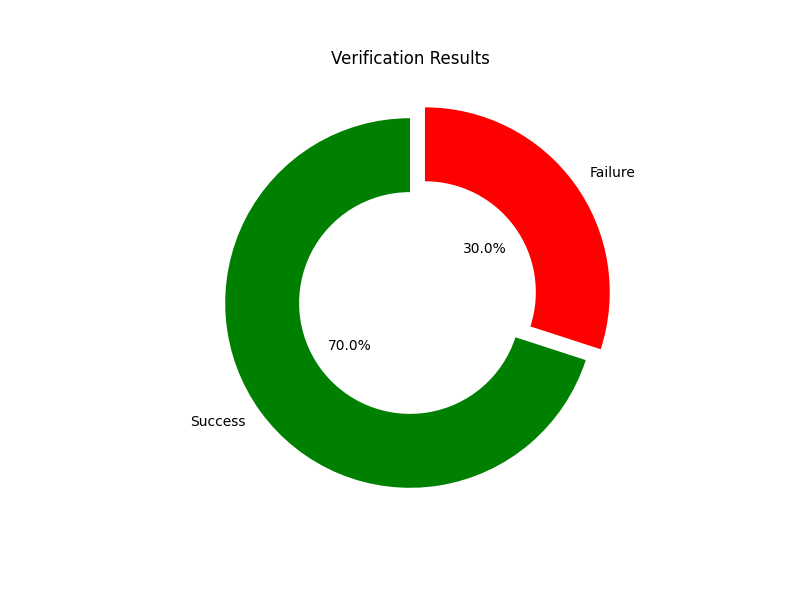
\includegraphics[width=0.85\textwidth]{obrazky-figures/deepface_verification_results.png}
	\caption{Kruhový diagram pro zobrazení úspěšnosti porovnání obličejů rámcem Deepface. Zelená část značí shodu v porovnání (\textit{Success}) a červená značí neúspěch (\textit{Failure}).}
        \label{fig:pie-chart-deepface}
\end{figure}

Z diagramu \ref{fig:pie-chart-deepface} je možné vidět, že 70 \% (175) dvojic bylo vyhodnoceno jako úspěšné a byla zde zjištěna shoda v podobnosti. Naopak 30 \% dvojic nebylo vyhodnoceno jako podobné a hodnota vzdálenosti vektorů \texttt{distance} u nich přesáhla práh podobnosti.

\bigskip

\noindent Druhá část experimentu prezentuje vypočtenou vzdálenost \texttt{distance} mezi dvěma vektory obličeje, kde nižší hodnota indikuje větší podobnost mezi dvojicemi. Vzdálenost je zobrazena pro všech 250 dvojic z provedeného experimentu v grafu \ref{fig:scatter-plot-deepface}. V grafu figuruje i červená přerušovaná čára, představující prahovou hodnotu \texttt{threshold}, která byla použita k rozhodnutí o podobnosti v předchozím experimentu. Všechny hodnoty vzdáleností pod touto čarou jsou vyhodnoceny jako shoda v porovnání. Prahová hodnota pro tento experiment byla 0,68.

\begin{figure}[H]
	\centering
	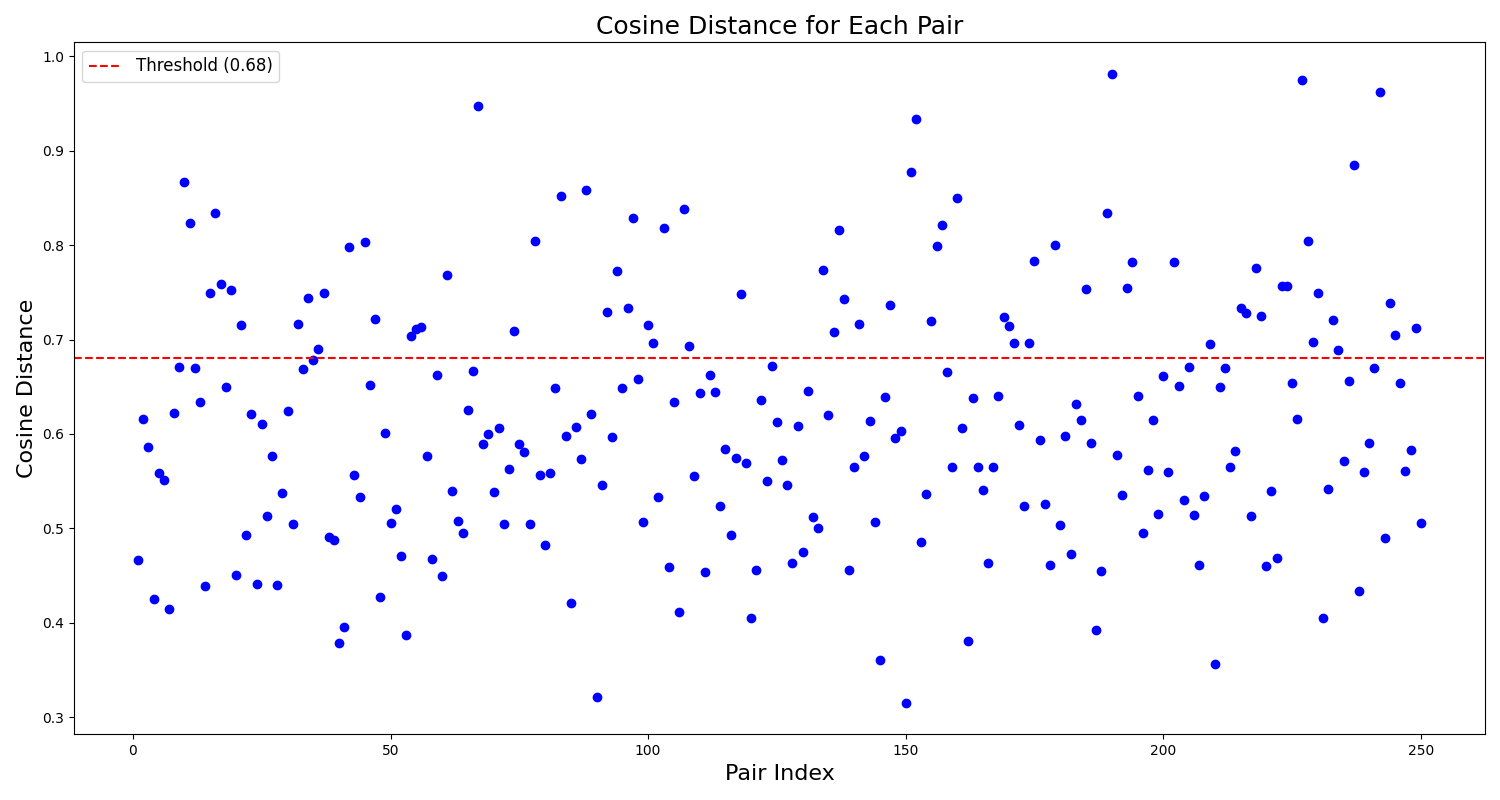
\includegraphics[width=1\textwidth]{obrazky-figures/deepface_face_distances.png}
	\caption{Korelační diagram pro zobrazení vzdálenosti vektorů dvojic snímků obličejů. Červená přerušovaná čára zastupuje prahovou hodnotu (\textit{threshold}), rozhodující o úspěšnosti porovnání.}
        \label{fig:scatter-plot-deepface}
\end{figure}

Diagram \ref{fig:scatter-plot-deepface} zobrazuje grafické znázornění výsledků vyhodnocujících podobnost dvojic. Při bližším zkoumaní hodnot determinující úspěšnost při předchozí část experimentu bylo zjištěno, že průměrná hodnota vzdálenosti \texttt{distance} byla 0,61577 a medián hodnot byl 0,60772. Obě hodnoty se nacházejí pod prahovou hodnotou 0,68, podporující vyšší úspěšnost s předchozí části experimentu.

Nejnižší naměřená hodnota vzdálenosti byla 0,3153, zaznamenána u páru označeného číslem 150. Nejvyšší vypočítaná hodnota byla 0,9815 u páru 190, s nejmenší podobností. Více o extrémech v hodnotách vzdáleností v sekci \ref{combinates-analysis}.

\bigskip

\noindent Nejvíce dvojic se vyskytovalo v rozmezí od 0,5 do 0,6 -- konkrétně se jednalo o 74 párů, což představuje 29,6 \% všech dvojic. Nejméně zastoupený byl interval 0,9 až 1, kde bylo zaznamenáno pouze 5 výskytů, tvořící 2 \% všech vzdáleností. Procentuální zastoupení vzdáleností pro všechny intervaly jsou na obrázku \ref{fig:plot-intervals}.

\begin{figure}[H]
	\centering
	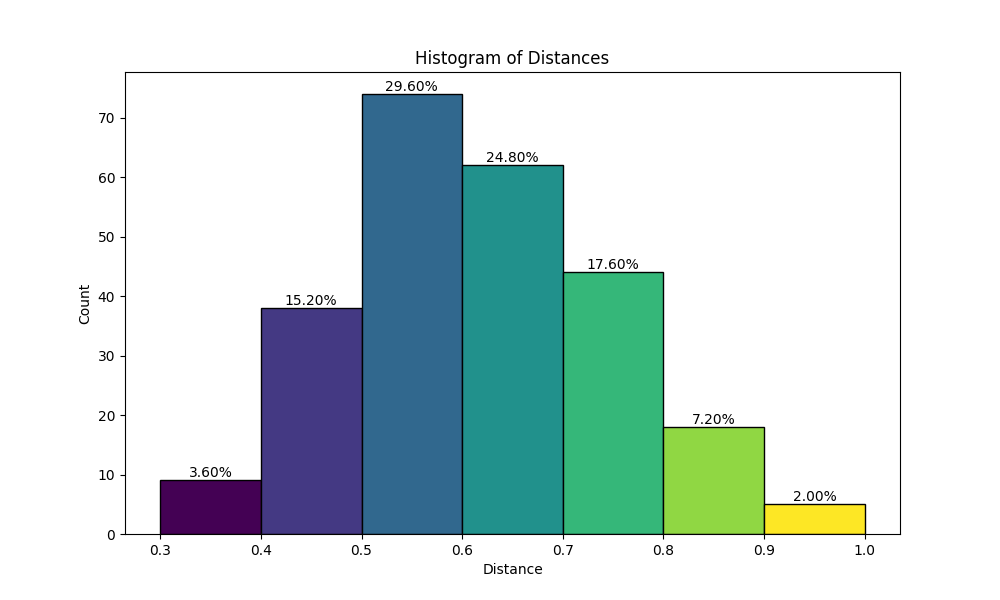
\includegraphics[width=1\textwidth]{obrazky-figures/deepface_distance_histogram.png}
	\caption{Procentuální zastoupení na intervalech pro všechny naměřené vzdálenosti.}
        \label{fig:plot-intervals}
\end{figure}

\noindent Tento experiment přináší podrobný pohled na úspěšnost porovnání identit mezi dvojicemi reálných a uměle vytvořených snímků obličeje, stejně jako na rozdíly v jejich vektorových reprezentacích s podrobným pohledem na tyto hodnoty. Současně připravuje půdu pro kombinované experimenty spojením s naměřenými hodnotami antropometrické analýzy.

\section{Kombinovaná analýza}
\label{combinates-analysis}

Experimenty v této sekci budou pracovat s výsledky z předchozích experimentů a budou kombinovat oba použité modely a jejich výstupy, pro podrobnější zkoumání. Hlavním účelem bude zkoumat podobnost dat mezi modely a zjistit, zda extrémní hodnoty u jednoho modelu kopírují hodnoty u modelu druhého. Konkrétně budou analyzovány dvojice s nejvyššími a nejnižšími hodnotami vzdálenosti podle rámce Deepface. U těchto nově vytvořených podskupin bude provedena antropometrická analýza modelem MediaPipe a vyhodnotí se, zda jsou zde také data nakloněné k extrému.

\subsection*{Dvojice s nejvyšší vzdáleností vektorů}

Výskytů s hodnotou vzdálenosti vektorů obličeje vyšší než 0,9 bylo pouze 5 z celkového počtu 250 zkoumaných dvojic. Tyto páry měly nejvyšší srovnávací hodnoty v rámci celé studie, což naznačuje, že obličeje by měly být nejvíce odlišné. Tabulka \ref{tab:high-distances} ukazuje konkrétní hodnoty vzdáleností mezi těmito páry, získané pomocí funkce rámce Deepface rozšířené a průměrnou hodnotu rozdílů vzdáleností modelu MediaPipe.

\begin{table}[H]
        \centering
        \renewcommand{\arraystretch}{1.15}
        \begin{tabular}{|c|c|c|}
                \hline
                Označení snímku & Vzdálenost Deepface & Průměrná vzdálenost MediaPipe \\
                \hline
                067 & 0,9469 & 0,0104 \\
                152 & 0,9335 & 0,0087 \\
                190 & 0,9815 & 0,0067 \\
                227 & 0,9753 & 0,0103 \\
                242 & 0,9625 & 0,0079 \\
                \hline
        \end{tabular}
        \caption{Tabulku zahrnující nejvyšší spočítané vzdálenosti vektorů pro dvojice snímků.}
        \label{tab:high-distances}
\end{table}

Hodnoty antropometrického měření u této skupiny jsou vyšší než obecný průměr 0,00633 všech dvojic. Průměrná hodnota u modelu MediaPipe v této skupině činí 0,0088. Vyšší vzdálenost byla tedy zjištěna nejen při analýze pomocí modelu Deepface, ale také při analýze modelem MediaPipe.

\subsection*{Dvojice s nejnižší vzdáleností vektorů}

Obdobně jako předchozí podsekce se zde pracuje s hodnotami vzdáleností od rámce Deepface, zde se ale jedná o ty nejnižší, tedy ty páry, které si byly nejvíce podobné. Pracuje se zde s dvojicemi s hodnotou nižší než 0,4. Jedná se o 9 z celkového počtu 250 zkoumaných dvojic, tvořící 3,6 \% výsledků. Výsledky vzdáleností jsou zobrazeny v tabulce \ref{tab:low-distances}, společně s hodnotami měření modelu MediaPipe.

\begin{table}[H]
        \centering
        \renewcommand{\arraystretch}{1.15}
        \begin{tabular}{|c|c|c|}
                \hline
                Označení snímku & Vzdálenost Deepface & Průměrná vzdálenost MediaPipe \\
                \hline
                040 & 0,3788 & 0,0053 \\
                041 & 0,3952 & 0,0049 \\
                053 & 0,3869 & 0,0057 \\
                090 & 0,3210 & 0,0055 \\
                145 & 0,3606 & 0,0051 \\
                150 & 0,3153 & 0,0062 \\
                162 & 0,3805 & 0,0095 \\
                187 & 0,3921 & 0,0044 \\
                210 & 0,3567 & 0,0052 \\
                \hline
        \end{tabular}
        \caption{Tabulku zahrnující nejnižší spočítané vzdálenosti vektorů pro dvojice snímků.}
        \label{tab:low-distances}
\end{table}

U skupiny s nejvyšší podobností a nejnižší vzdáleností byla spočítána průměrná hodnota pro model MediaPipe ve výši 0,0057, což odpovídá výsledkům získaným od rámce Deepface. Průměrná hodnota vzdáleností jednotlivých proporcí je výrazně nižší než celkový průměr modelu MediaPipe, který je 0,0063.

\bigskip

\noindent Experimenty se zaměřily na zkoumání extrémních hodnot (vysoké a nízké) obou modelů, aby zjistily, zda jsou v souladu. V obou experimentech bylo prokázáno, že vyšší hodnoty získané z jednoho modelu vedou k vyšším hodnotám z modelu druhého modelu. Totéž platí i pro nižší hodnoty; pokud model první generuje nižší hodnoty, model druhý bude vykazovat podobný trend. To znamená, že výsledky experimentů jsou vzájemně konzistentní a podporují hypotézu, že oba modely sdílejí podobné trendy v měření a analýzách.

\section{Obecný pohled na dvojice}
\label{personal-evaluation}

V této sekci bude představen autorův osobní pohled na rozdílnost reálných a uměle vygenerovaných snímků obličeje. Zkoumány budou dvě dvojice, každá z opačného spektra skupin minimálních a maximálních vzdáleností vektorů uvedených v sekci \ref{combinates-analysis}. Ke konkrétním dvojicím bude doplněn komentář o rozdílech mezi obličeji, včetně upozornění na případně vzniklé artefakty a jejich rozsáhlost.

\bigskip

\noindent První zkoumanou dvojicí budou snímky obličeje s pořadovým číslem 242, patřící do skupiny s nejvyšším rozdílem vzdáleností vektorů a z technické stránky tedy jedna z nejvíce lišících se dvojic. Oba snímky jsou na obrázku \ref{fig:personal-242}.

\begin{figure}[H]
    \centering
    \begin{subfigure}{0.45\textwidth}
         \centering
         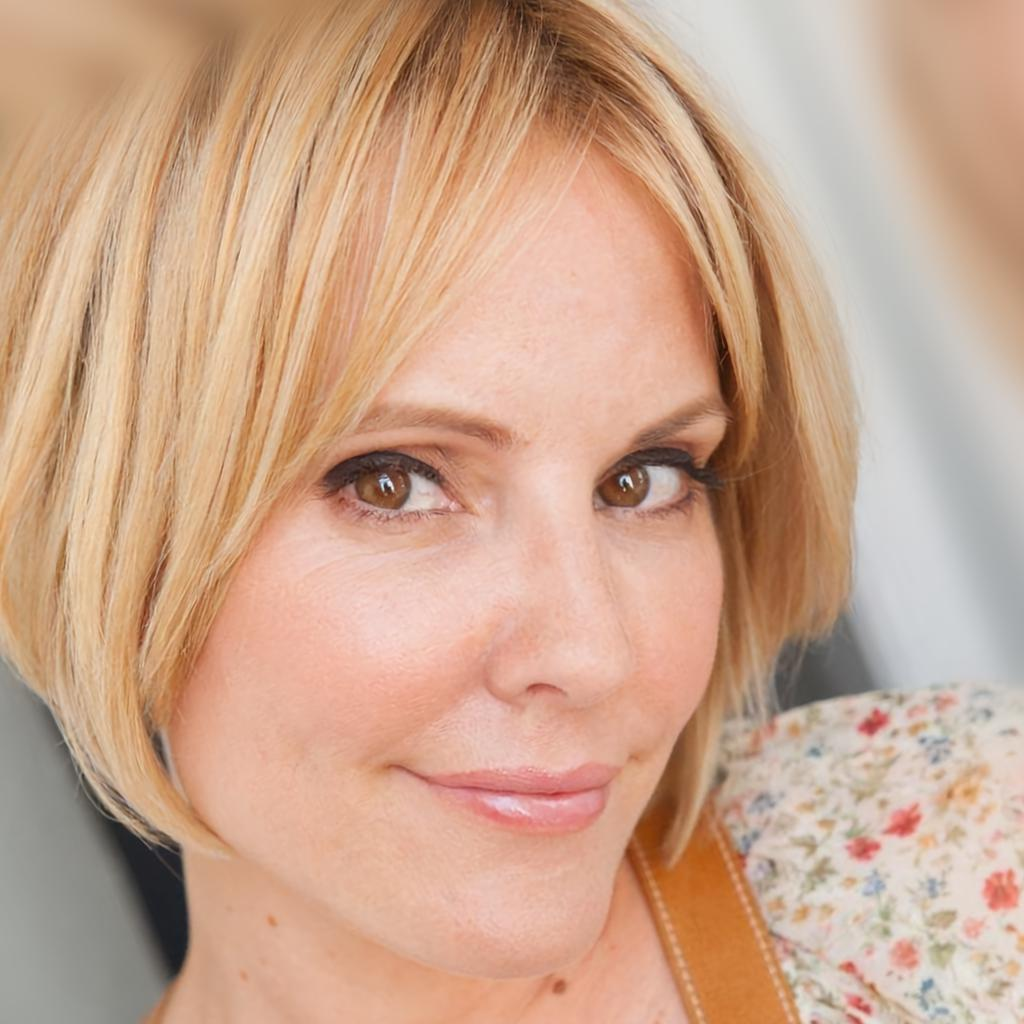
\includegraphics[width=1\textwidth]{obrazky-figures/real-242.jpg}
         \caption{Původní snímek obličeje}
         \label{fig:personal-242-real}
     \end{subfigure}
     \hfill
     \begin{subfigure}{0.45\textwidth}
         \centering
         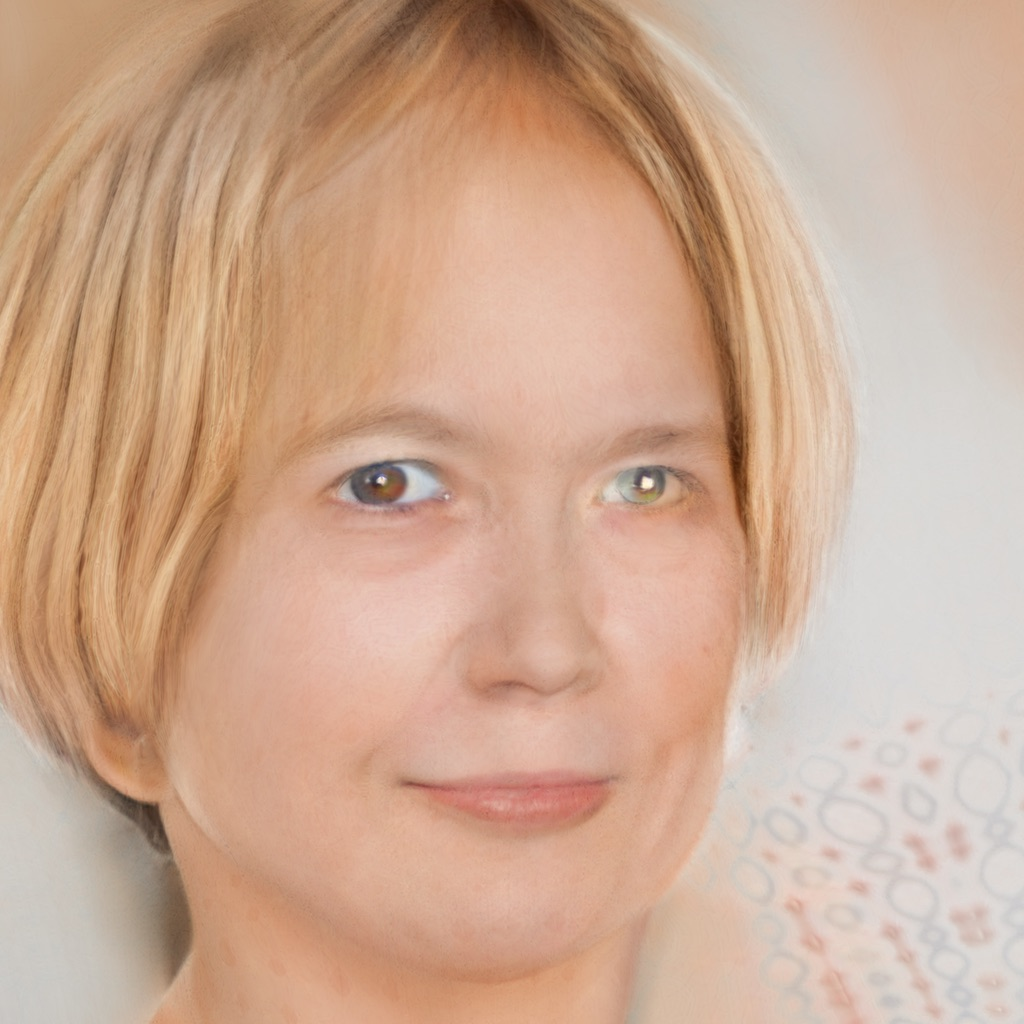
\includegraphics[width=1\textwidth]{obrazky-figures/gen-242.jpeg}
         \caption{Umělý vygenerovaný snímek obličeje}
         \label{fig:personal-242-gen}
     \end{subfigure}
    \caption{Porovnání reálného a vygenerovaného snímku obličeje modelem StyleGAN3 s vysokou hodnotou vzdálenosti mezi vektory obličeje.}
    \label{fig:personal-242}
\end{figure}

O dvojici lze říci, že se na první pohled jeví jako velmi odlišná. Jeden ze spojujících prvků jsou vlasy, kterým zůstal stejný odstín jako na původním snímku. Co se týče proporcí -- šířka obličeje je výrazně větší u generovaného snímku, to stejné lze říct i o šířce čelisti. Rozdíl ve výšce již tolik vidět nelze. Výrazný rozdíl lze sledovat dále u úst, které disponují úplně odlišným tvarem, podobná situace nastala i u očí, kde došlo i k výrazné změně barvy u obou očí a k odlišnému natočení pohledu. Artefaktem vystupující na vygenerovaném snímku je ucho, které je položené pod vlasy na levé straně tváře. Tváře ztratily lehce načervenalou barvu, ta se proměnila na více neutrální, korespondující se zbytkem obličeje.

\bigskip

\noindent Druhou zkoumanou dvojicí budou snímky obličeje s pořadovým číslem 90, patřící naopak do skupiny s nejnižším rozdílem vzdáleností vektorů. Reálný i vygenerovaný snímek jsou na obrázku \ref{fig:personal-090}.

\begin{figure}[H]
    \centering
    \begin{subfigure}{0.45\textwidth}
         \centering
         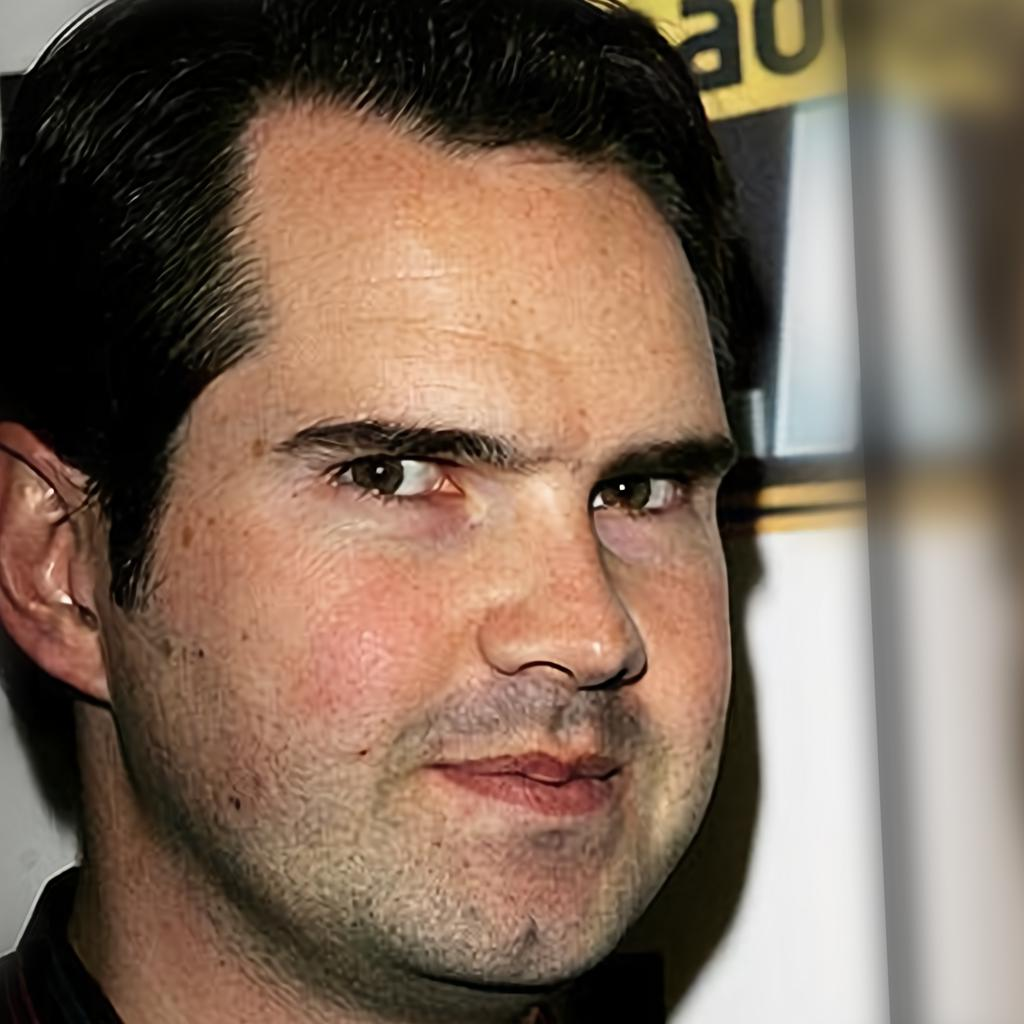
\includegraphics[width=1\textwidth]{obrazky-figures/real-090.jpg}
         \caption{Původní snímek obličeje}
         \label{fig:personal-090-real}
     \end{subfigure}
     \hfill
     \begin{subfigure}{0.45\textwidth}
         \centering
         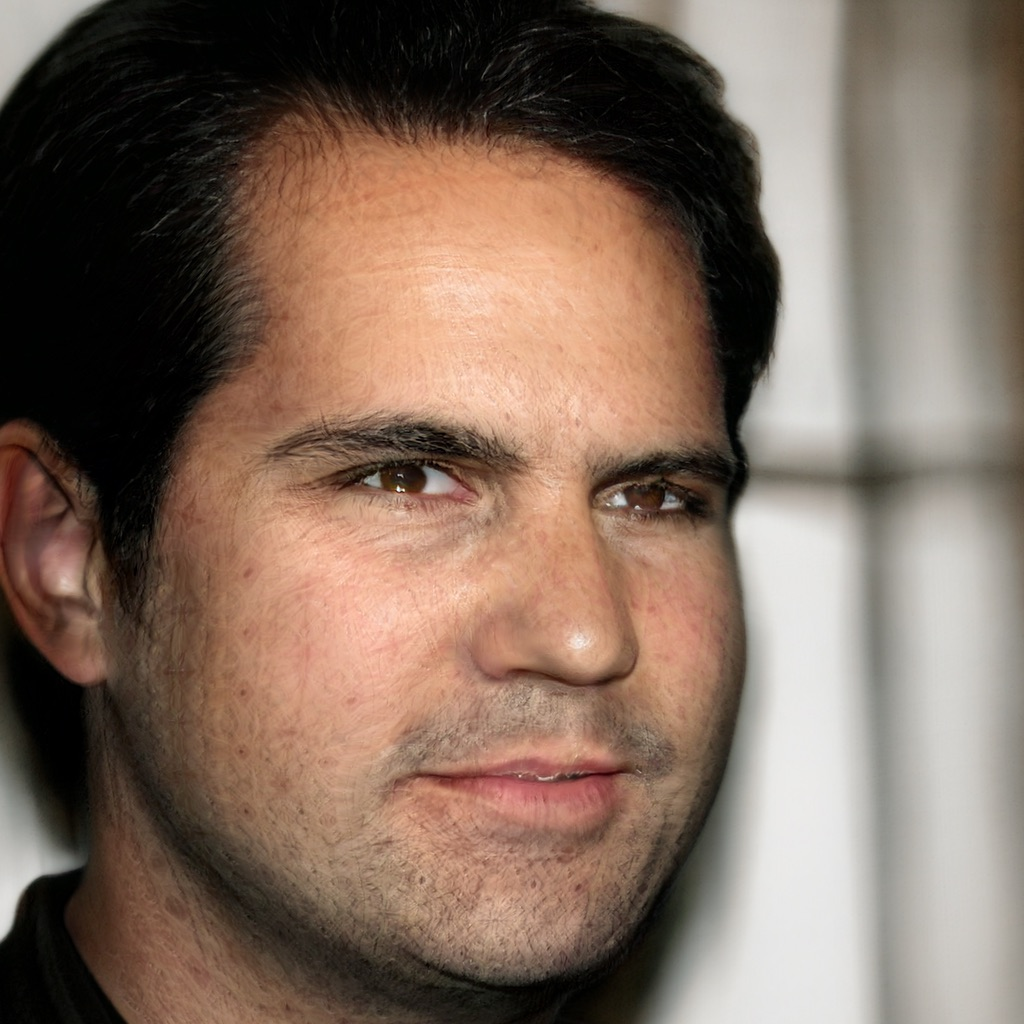
\includegraphics[width=1\textwidth]{obrazky-figures/gen-090.jpeg}
         \caption{Umělý vygenerovaný snímek obličeje}
         \label{fig:personal-090-gen}
     \end{subfigure}
    \caption{Porovnání reálného a vygenerovaného snímku obličeje modelem StyleGAN3 s nízkou hodnotou vzdálenosti mezi vektory obličeje.}
    \label{fig:personal-090}
\end{figure}

Podobně jako u předchozí dvojice zde dochází k výrazným změnám u očí a úst jedince. Oči jsou výrazně menší a ústa jsou naopak mírně širší. Šířka a výška obličeje zůstává v~tomto případě poměrně podobná původnímu snímku. Kromě specifické textury obličeje, pravděpodobně způsobené nižší kvalitou původní fotografie, nejsou přítomny žádné další anomálie nebo artefakty. Stejně jako u předchozí dvojice vymizela při generování lehká červená barva pokrývající tváře obličeje, která se přetvořila na více neutrální odstín pokrývající zbytek obličeje. Nos u dvojice se výrazně změnil – stal se kulatějším a méně širokým než na původní fotografii.

\bigskip

\noindent Z prozkoumaných dvojic snímků je vidět trend v odlišnosti rozměrů a vzhledu očí a úst. Dále se u obou příkladů měnil barevný profil tváře na více neutrální. U dvojice s vyšší vzdáleností vektorů obličeje byl viditelnější rozdíl v šířce obličeje a čelisti, jedná se o dvě nejvíce lišící se proporce, tedy i o faktor, který nejvíce rozhodoval o neúspěšném vyhodnocení podobnosti dvojice.

\chapter{Závěr}
\label{zaver}

Tato práce se zaměřuje na dvě hlavní oblasti: detekci a zkoumání antropometrických bodů na obličeji a generování uměle vytvořených snímků obličeje pomocí sítí GAN. Došlo k prozkoumání toho, které antropometrické body jsou na obličeji významné a jaké proporce lze měřit a analyzovat. Byl vybrán model pro generování snímků obličeje, který využívá reálný snímek jako zdroj pro generování. 

V rámci antropometrické analýzy bylo nahlíženo na významné proporce na obličeji jednotlivců a z kterých antropometrických bodů se skládají. Proporce zahrnují různé rozměry obličeje, jako je šířka a výška obličeje, šířka oka, vzdálenost očí od sebe, výška nosu, šířka úst a šířka čelisti. Kromě toho se měří další klíčové oblasti, například délka nosu, vzdálenost mezi nosem a ústy, nebo výška rtů.

Při výběru modelu pro generování umělých snímků obličeje bylo prozkoumáno několik možností, které byly vyhodnoceny z hlediska přesnosti, kvality a schopnosti generovat realistické snímky. Jako nejvhodnější a nejpokročilejší model byl shledán model StyleGAN3, který se vyznačuje pokročilými schopnostmi v oblasti generování detailních a realistických obličejů. V práci zastupuje roli pro dotvoření dvojic reálných snímků podmnožiny datové sady CelebAMask-HQ.

V práci se podařilo vyhodnotit dvojice reálných a umělých snímků obličeje dvěma způsoby. Prvním byla antropometrická analýza modelem MediaPipe, která poskytovala mapu antropometrických bodů na obličeji. Byly měřeny jednotlivé definované proporce a porovnány v rámci dvojic snímků. Následně byly vybrány proporce, které se u dvojic lišily nejvíce. Největší rozdíly byly zaznamenány v šířce obličeje, čelisti a úst, stejně jako ve výšce obličeje. Naopak menší rozdíly byly zjištěny ve výšce horního a dolního rtu nebo šířce oka. Celkový poměr obličeje u reálných snímků dosáhl 91,37 \% a u umělých snímků 89,92 \%. Tato rozdílná hodnota je relativně malá a naznačuje lehkou odlišnost.

Druhý způsob zastupoval rámec Deepface, který poskytoval srovnání dvojic na základě výpočtu jejich kosinové vzdáleností. Z 250 zkoumaných dvojic bylo 175 vyhodnoceno jako podobných, tvořící 70 \%. Průměrný hodnota vzdálenosti byla 0,6158, přičemž prahová hodnota pro rozhodnutí o podobnosti byla 0,68. Jakákoli hodnota pod touto mezí byla považována za podobný výsledek.

Z pohledu dalšího vývoje dává smysl prozkoumat i oblast difúzních modelů pro generování obličeje a provést antropometrickou analýzu i zde. Difúzní modely jsou dnes již velice známé a jejich popularita stále roste i v široké veřejnosti.



%===============================================================================

% Pro kompilaci po částech (viz projekt.tex) nutno odkomentovat
%\end{document}
